

%\newcommand*{\ACM}{}%

\ifdefined\ACM

%\documentclass[sigplan,screen]{acmart}
\documentclass[manuscript,screen,review]{acmart}

\else
  \documentclass[18pt]{article}
\usepackage{libertine}
\usepackage{cuted}
%\usepackage{widetext}
\usepackage[utf8]{inputenc}
\usepackage[a4paper, total={6in, 9in}]{geometry}
\usepackage{braket}
\usepackage{xcolor}
\usepackage{amsmath}
\usepackage{amsfonts}
\usepackage{amsthm}
\usepackage{amssymb}
%\usepackage[ocgcolorlinks]{hyperref}
\usepackage{hyperref}
%\usepackage{hyperref,xcolor}
%\usepackage[ocgcolorlinks]{ocgx2}
\usepackage{cleveref}
\usepackage{graphicx}
\usepackage{svg}
\usepackage{float}
\usepackage{tikz}
\usetikzlibrary{patterns, shapes.arrows}
\usepackage{adjustbox}
%\usepackage{tikz-network}
\usepackage{tkz-graph}
\usepackage{tkz-berge}
\usepackage[linesnumbered]{algorithm2e}
\usepackage{multicol}
\usepackage[backend=biber,style=alphabetic,sorting=ynt]{biblatex}
%\usepackage{xcolor}
%\usepackage{tkz-berge}
%\usepackage{tkz-graph}
\usepackage{pgfplots}
\usepackage{sagetex}
\usepackage{setspace}
\usepackage{etoc}
%\usepackage{wrapfig}
\usepackage{pgfgantt}
\DeclareUnicodeCharacter{2212}{−}
\usepgfplotslibrary{groupplots,dateplot}
\pgfplotsset{compat=newest}

\newtheorem{theorem}{Theorem}
\newtheorem{definition}{Definition}
\newtheorem{example}{Example}
\newtheorem{claim}{Claim}
\newtheorem{fact}{Fact}
\newtheorem{remark}{Remark}
\newtheorem*{theorem*}{Theorem}
\newtheorem{lemma}{Lemma}
\crefname{lemma}{Lemma}{Lemmas}
\hypersetup{colorlinks=true}
% , allcolors=blue,allbordercolors=blue,pdfborderstyle={0 0 1}}
%\hypersetup{pdfborder={2 2 2}}
% pdfpagemode=FullScreen,
% backref 

\newtheorem{problem}{Problem}
\crefname{problem}{Problem}{Problems}

\DeclareMathOperator{\Ima}{Im}


\usepackage{cancel}
\usepackage{subcaption}
\addbibresource{./sample.bib}

\fi

\begin{document}
\newcommand{\commentt}[1]{\textcolor{blue}{ \textbf{[COMMENT]} #1}}
\newcommand{\ctt}[1]{\commentt{#1}}
\newcommand{\prb}[1]{ \mathbf{Pr} \left[ #1 \right]}
\newcommand{\prbm}[2]{ \mathbf{Pr}_{ #2 }\left[ #1 \right]}
\newcommand{\prbc}[3]{ \mathbf{Pr}_{ #2 }\left[ #1 \right | #3]}
\newcommand{\prbcprb}[3]{ \prbc{#2}{#1}{#3} \cdot \prb{#3} } 
\newcommand{\expp}[1]{ \mathbf{E} \left[ {#1} \right]}
\newcommand{\onotation}[1]{\(\mathcal{O} \left( {#1}  \right) \)}
\newcommand{\ona}[1]{\onotation{#1}}
\newcommand{\PSI}{{\ket{\psi}}}
\newcommand{\xij} { X_{ij} } 
\DeclareMathOperator{\Ima}{Im}
%\newcommand{\LESn}{\ket{\psi_n}}
%\newcommand{\LESa}{\ket{\phi_n}}
%\newcommand{\LESs}{\frac{1}{\sqrt{n}}\sum_{i}{\ket{\left(0^{i}10^{n-i}\right)^{n}}}}
%\newcommand{\Hn}{\mathcal{H}_{n}}
%\newcommand{\Ep}{\frac{1}{\sqrt{2^n}}\sum^{2^n}_{x}{ \ket{xx}}}
%\newcommand{\HON}{\ket{\psi_{\text{honest}}}}
%\newcommand{\Lemma}{\paragraph{Lemma.}}
\newcommand{\Cpa}{[n, \rho n, \delta n]}
%\setlength{\columnsep}{0.6cm}
\newcommand{\Jvv}{ \bar{J_{v}} } 
\newcommand{\Cvv}{ \tilde{C_{v}} } 

\newcommand{\Gz}{ G_{z}^{\delta} } 
\newcommand{ \Tann } {  \mathcal{T}\left( G, C_0 \right) }
\newcommand{\ireducable}{ireducable \hyperref[ire]{[\ref{ire}]} }
\newcommand{\cutUU}{E(U_{-1} \bigcup U_{+1} ,U)} 
\newcommand{\wcutUU}{w\left( E(U_{-1} \bigcup U_{+1} ,U)  \right)}
\newcommand{\testgo}{  \mathcal{T}\left(J, q , C_{0}\right) } 

\newcommand{\duC}{\left( C_{A}^{\perp}\otimes C_{B}^{\perp} \right)^{\perp}}
\newcommand{\duduC}{\left( C_{A}\otimes C_{B}\right)^{\perp}}
  




%\title{ $\textbf{QNC}_{1} \subset $ noisy-\textbf{BQP}}
\title{ On The Cost of Fault-Tolerainzing Shallow Circuits. }
\author{Michael Ben-Or \ \ David Ponarovsky}
\maketitle

\newcommand*{\Mbas}{\mathcal{X}^\prime}
\newcommand*{\bas}{\mathcal{X}}
\newcommand*{\sMbas}{\Mbas}
\newcommand*{\QQ}{C_{X}/C_{Z}^\perp }
\newcommand*{\trig}{ Triorthogonal }
\newcommand*{\Hyp}{ Hyperproduct }
\newcommand*{\Cin}{ C_{\text{initial}} }
\newcommand*{\Ctan}{ C_{\text{Tan}} }



\newcommand*{\QACze}{ \mathbf{QAC}_{0} }
\newcommand*{\QNCzef}{ \mathbf{QNC}_{0,f} }
\newcommand*{\QNCon}{ \mathbf{QNC}_{1} }
\newcommand*{\NCon}{ \mathbf{NC}_{1} }
\newcommand*{\noiseQNCon}{ noisy-$\QNCon$ }


\abstract{In this work we study the overall depth overhead cost required for constructing fault tolerance circuits. We focus on shallow depth circuits classes, In particular, $\QACze, \QNCzef$ and $\QNCon$ and certain knowns problem candidates for demonstrating quantum advantage such as factoring \cite{Shor_1997} and Instantaneous Quantum Polynomial-time \cite{Bremner_2017}, \cite{Paletta_2024}. We only give a partial answers, Yet, clues that might pave the way towards a full understanding of the complexity versus fault tolerance trade-off. 

  \section{Introduction.} The question about the feasibility of computation under noise is almost as ancient as the computer science field itself, initialized by Von Neumann \cite{Neumann+1956+43+98} at the time that classical computation putted in debuts. Time been pass and the followed works had pointed that not even a polynomial computation in the presence of noise is still reasonable but one can implement a fault tolerance version at a most constant times cost at the circuits depth \cite{Pippenger}. Or in asymptotic sense, classical computation in the presence of noise is as exactly hard as computation in ideal environment.  

  Once again, the feasibility question raised again, this time regarding quantum computing, and while an intensive work has been done, and also succeed to prove that polynomial quantum computation can be made fault tolerance, \cite{aharonov1999faulttolerant},\cite{gottesman2014faulttolerant} and even with only constant overhead at the original circuit width \cite{grospellier:tel-03364419}, the required depth over-head is till not well understood. We stress out that in all the familiar constructions, in construct to Pippenger \cite{Pippenger}, original constant-depth gates are mapped to asymptotically grow\footnote{Note, that here, classical computation is also counted in the overall depth cost} depth gates. 
  
  This work address the above, We ask whether a magnitude depth overhead is an unavoidable price that one has to pay. And, in particular, whether an ideal $\QNCon$ circuits can be computed in noisy-$\QNCon$ circuits. We show how using the ideas presented in \cite{grospellier:tel-03364419} and \cite{Pippenger} gives almost immediately $\QNCzef \subset$ \noiseQNCon and that sampling from IQP \cite{Bremner_2017} also can be done in logarithmic depth circuits.    
  \section{ Notations. } In the following we present the notations used in the paper, readers who familiar with the literature of coding theory and quantum fault tolerance might skip \Cref{sec:classical} and \Cref{sec:quantum} and continue directly to \Cref{sec:decoders} which introduces less standard notations. 



  \begin{figure}[h]
\begin{subfigure}[h]{0.05\textwidth}
      \
    \end{subfigure}
    \begin{subfigure}[h]{0.45\textwidth}

  Once again, the feasibility question raised again, this time regarding quantum computing, and while an intensive work has been done, and also succeed to prove that polynomial quantum computation can be made fault tolerance, \cite{aharonov1999faulttolerant},\cite{gottesman2014faulttolerant} and even with only constant overhead at the original circuit width \cite{grospellier:tel-03364419}, the required depth over-head is till not well understood. We stress out that in all the familiar constructions, in construct to Pippenger \cite{Pippenger}, original constant-depth gates are mapped to asymptotically grow\footnote{Note, that here, classical computation is also counted in the overall depth cost} depth gates. 
    \end{subfigure}
    \begin{subfigure}[h]{0.05\textwidth}
      \
    \end{subfigure}
    \begin{subfigure}[h]{0.30\textwidth} 

    %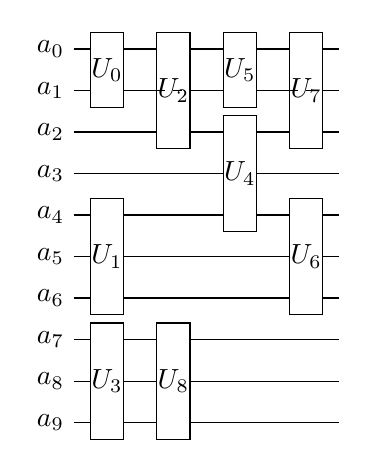
\begin{tikzpicture}[scale=1.000000,x=1pt,y=1pt]
\filldraw[color=white] (0.000000, -7.500000) rectangle (96.000000, 142.500000);
% Drawing wires
% Line 1: a0 W a_0
\draw[color=black] (0.000000,135.000000) -- (96.000000,135.000000);
\draw[color=black] (0.000000,135.000000) node[left] {$a_0$};
% Line 2: a1 W a_1
\draw[color=black] (0.000000,120.000000) -- (96.000000,120.000000);
\draw[color=black] (0.000000,120.000000) node[left] {$a_1$};
% Line 3: a2 W a_2
\draw[color=black] (0.000000,105.000000) -- (96.000000,105.000000);
\draw[color=black] (0.000000,105.000000) node[left] {$a_2$};
% Line 4: a3 W a_3
\draw[color=black] (0.000000,90.000000) -- (96.000000,90.000000);
\draw[color=black] (0.000000,90.000000) node[left] {$a_3$};
% Line 5: a4 W a_4
\draw[color=black] (0.000000,75.000000) -- (96.000000,75.000000);
\draw[color=black] (0.000000,75.000000) node[left] {$a_4$};
% Line 6: a5 W a_5
\draw[color=black] (0.000000,60.000000) -- (96.000000,60.000000);
\draw[color=black] (0.000000,60.000000) node[left] {$a_5$};
% Line 7: a6 W a_6
\draw[color=black] (0.000000,45.000000) -- (96.000000,45.000000);
\draw[color=black] (0.000000,45.000000) node[left] {$a_6$};
% Line 8: a7 W a_7
\draw[color=black] (0.000000,30.000000) -- (96.000000,30.000000);
\draw[color=black] (0.000000,30.000000) node[left] {$a_7$};
% Line 9: a8 W a_8
\draw[color=black] (0.000000,15.000000) -- (96.000000,15.000000);
\draw[color=black] (0.000000,15.000000) node[left] {$a_8$};
% Line 10: a9 W a_9
\draw[color=black] (0.000000,0.000000) -- (96.000000,0.000000);
\draw[color=black] (0.000000,0.000000) node[left] {$a_9$};
% Done with wires; drawing gates
% Line 12: a0 a1 G  $ U_{0} $
\draw (12.000000,135.000000) -- (12.000000,120.000000);
\begin{scope}
\draw[fill=white] (12.000000, 127.500000) +(-45.000000:8.485281pt and 19.091883pt) -- +(45.000000:8.485281pt and 19.091883pt) -- +(135.000000:8.485281pt and 19.091883pt) -- +(225.000000:8.485281pt and 19.091883pt) -- cycle;
\clip (12.000000, 127.500000) +(-45.000000:8.485281pt and 19.091883pt) -- +(45.000000:8.485281pt and 19.091883pt) -- +(135.000000:8.485281pt and 19.091883pt) -- +(225.000000:8.485281pt and 19.091883pt) -- cycle;
\draw (12.000000, 127.500000) node {$ U_{0} $};
\end{scope}
% Line 13: a4 a5 a6 G $ U_{1} $
\draw (12.000000,75.000000) -- (12.000000,45.000000);
\begin{scope}
\draw[fill=white] (12.000000, 60.000000) +(-45.000000:8.485281pt and 29.698485pt) -- +(45.000000:8.485281pt and 29.698485pt) -- +(135.000000:8.485281pt and 29.698485pt) -- +(225.000000:8.485281pt and 29.698485pt) -- cycle;
\clip (12.000000, 60.000000) +(-45.000000:8.485281pt and 29.698485pt) -- +(45.000000:8.485281pt and 29.698485pt) -- +(135.000000:8.485281pt and 29.698485pt) -- +(225.000000:8.485281pt and 29.698485pt) -- cycle;
\draw (12.000000, 60.000000) node {$ U_{1} $};
\end{scope}
% Line 15: a7 a8 a9 G $ U_{3} $
\draw (12.000000,30.000000) -- (12.000000,0.000000);
\begin{scope}
\draw[fill=white] (12.000000, 15.000000) +(-45.000000:8.485281pt and 29.698485pt) -- +(45.000000:8.485281pt and 29.698485pt) -- +(135.000000:8.485281pt and 29.698485pt) -- +(225.000000:8.485281pt and 29.698485pt) -- cycle;
\clip (12.000000, 15.000000) +(-45.000000:8.485281pt and 29.698485pt) -- +(45.000000:8.485281pt and 29.698485pt) -- +(135.000000:8.485281pt and 29.698485pt) -- +(225.000000:8.485281pt and 29.698485pt) -- cycle;
\draw (12.000000, 15.000000) node {$ U_{3} $};
\end{scope}
% Line 14: a0  a2  G $ U_{2} $
\draw (36.000000,135.000000) -- (36.000000,105.000000);
\begin{scope}
\draw[fill=white] (36.000000, 120.000000) +(-45.000000:8.485281pt and 29.698485pt) -- +(45.000000:8.485281pt and 29.698485pt) -- +(135.000000:8.485281pt and 29.698485pt) -- +(225.000000:8.485281pt and 29.698485pt) -- cycle;
\clip (36.000000, 120.000000) +(-45.000000:8.485281pt and 29.698485pt) -- +(45.000000:8.485281pt and 29.698485pt) -- +(135.000000:8.485281pt and 29.698485pt) -- +(225.000000:8.485281pt and 29.698485pt) -- cycle;
\draw (36.000000, 120.000000) node {$ U_{2} $};
\end{scope}
\draw[color=black,dashed] (30.000000, 120.000000) -- (42.000000, 120.000000);
% Line 20: a7 a8 a9 G $ U_{8} $
\draw (36.000000,30.000000) -- (36.000000,0.000000);
\begin{scope}
\draw[fill=white] (36.000000, 15.000000) +(-45.000000:8.485281pt and 29.698485pt) -- +(45.000000:8.485281pt and 29.698485pt) -- +(135.000000:8.485281pt and 29.698485pt) -- +(225.000000:8.485281pt and 29.698485pt) -- cycle;
\clip (36.000000, 15.000000) +(-45.000000:8.485281pt and 29.698485pt) -- +(45.000000:8.485281pt and 29.698485pt) -- +(135.000000:8.485281pt and 29.698485pt) -- +(225.000000:8.485281pt and 29.698485pt) -- cycle;
\draw (36.000000, 15.000000) node {$ U_{8} $};
\end{scope}
% Line 16: a2 a3 a4 G $ U_{4} $
\draw (60.000000,105.000000) -- (60.000000,75.000000);
\begin{scope}
\draw[fill=white] (60.000000, 90.000000) +(-45.000000:8.485281pt and 29.698485pt) -- +(45.000000:8.485281pt and 29.698485pt) -- +(135.000000:8.485281pt and 29.698485pt) -- +(225.000000:8.485281pt and 29.698485pt) -- cycle;
\clip (60.000000, 90.000000) +(-45.000000:8.485281pt and 29.698485pt) -- +(45.000000:8.485281pt and 29.698485pt) -- +(135.000000:8.485281pt and 29.698485pt) -- +(225.000000:8.485281pt and 29.698485pt) -- cycle;
\draw (60.000000, 90.000000) node {$ U_{4} $};
\end{scope}
% Line 17: a0 a1 G $ U_{5} $
\draw (60.000000,135.000000) -- (60.000000,120.000000);
\begin{scope}
\draw[fill=white] (60.000000, 127.500000) +(-45.000000:8.485281pt and 19.091883pt) -- +(45.000000:8.485281pt and 19.091883pt) -- +(135.000000:8.485281pt and 19.091883pt) -- +(225.000000:8.485281pt and 19.091883pt) -- cycle;
\clip (60.000000, 127.500000) +(-45.000000:8.485281pt and 19.091883pt) -- +(45.000000:8.485281pt and 19.091883pt) -- +(135.000000:8.485281pt and 19.091883pt) -- +(225.000000:8.485281pt and 19.091883pt) -- cycle;
\draw (60.000000, 127.500000) node {$ U_{5} $};
\end{scope}
% Line 18: a4 a5 a6 G $ U_{6} $
\draw (84.000000,75.000000) -- (84.000000,45.000000);
\begin{scope}
\draw[fill=white] (84.000000, 60.000000) +(-45.000000:8.485281pt and 29.698485pt) -- +(45.000000:8.485281pt and 29.698485pt) -- +(135.000000:8.485281pt and 29.698485pt) -- +(225.000000:8.485281pt and 29.698485pt) -- cycle;
\clip (84.000000, 60.000000) +(-45.000000:8.485281pt and 29.698485pt) -- +(45.000000:8.485281pt and 29.698485pt) -- +(135.000000:8.485281pt and 29.698485pt) -- +(225.000000:8.485281pt and 29.698485pt) -- cycle;
\draw (84.000000, 60.000000) node {$ U_{6} $};
\end{scope}
% Line 19: a0  a2  G $ U_{7} $
\draw (84.000000,135.000000) -- (84.000000,105.000000);
\begin{scope}
\draw[fill=white] (84.000000, 120.000000) +(-45.000000:8.485281pt and 29.698485pt) -- +(45.000000:8.485281pt and 29.698485pt) -- +(135.000000:8.485281pt and 29.698485pt) -- +(225.000000:8.485281pt and 29.698485pt) -- cycle;
\clip (84.000000, 120.000000) +(-45.000000:8.485281pt and 29.698485pt) -- +(45.000000:8.485281pt and 29.698485pt) -- +(135.000000:8.485281pt and 29.698485pt) -- +(225.000000:8.485281pt and 29.698485pt) -- cycle;
\draw (84.000000, 120.000000) node {$ U_{7} $};
\end{scope}
\draw[color=black,dashed] (78.000000, 120.000000) -- (90.000000, 120.000000);
% Done with gates; drawing ending labels
% Done with ending labels; drawing cut lines and comments
% Done with comments
\end{tikzpicture}

    \caption{location.}
    \label{fig:location}
    \end{subfigure} 
  \end{figure}

  \subsection{Classical and Quantum Circuits.} 
  \begin{definition}
    location $(i,j)$ of $C$. \ctt{Add here a figure of classical circuit, that demonstrates locations.}
  \end{definition}

%  \begin{figure}[h]
%    \centering
%    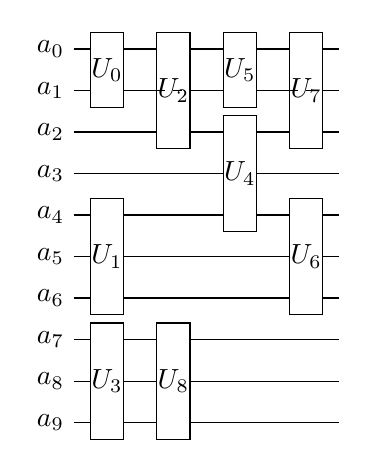
\begin{tikzpicture}[scale=1.000000,x=1pt,y=1pt]
\filldraw[color=white] (0.000000, -7.500000) rectangle (96.000000, 142.500000);
% Drawing wires
% Line 1: a0 W a_0
\draw[color=black] (0.000000,135.000000) -- (96.000000,135.000000);
\draw[color=black] (0.000000,135.000000) node[left] {$a_0$};
% Line 2: a1 W a_1
\draw[color=black] (0.000000,120.000000) -- (96.000000,120.000000);
\draw[color=black] (0.000000,120.000000) node[left] {$a_1$};
% Line 3: a2 W a_2
\draw[color=black] (0.000000,105.000000) -- (96.000000,105.000000);
\draw[color=black] (0.000000,105.000000) node[left] {$a_2$};
% Line 4: a3 W a_3
\draw[color=black] (0.000000,90.000000) -- (96.000000,90.000000);
\draw[color=black] (0.000000,90.000000) node[left] {$a_3$};
% Line 5: a4 W a_4
\draw[color=black] (0.000000,75.000000) -- (96.000000,75.000000);
\draw[color=black] (0.000000,75.000000) node[left] {$a_4$};
% Line 6: a5 W a_5
\draw[color=black] (0.000000,60.000000) -- (96.000000,60.000000);
\draw[color=black] (0.000000,60.000000) node[left] {$a_5$};
% Line 7: a6 W a_6
\draw[color=black] (0.000000,45.000000) -- (96.000000,45.000000);
\draw[color=black] (0.000000,45.000000) node[left] {$a_6$};
% Line 8: a7 W a_7
\draw[color=black] (0.000000,30.000000) -- (96.000000,30.000000);
\draw[color=black] (0.000000,30.000000) node[left] {$a_7$};
% Line 9: a8 W a_8
\draw[color=black] (0.000000,15.000000) -- (96.000000,15.000000);
\draw[color=black] (0.000000,15.000000) node[left] {$a_8$};
% Line 10: a9 W a_9
\draw[color=black] (0.000000,0.000000) -- (96.000000,0.000000);
\draw[color=black] (0.000000,0.000000) node[left] {$a_9$};
% Done with wires; drawing gates
% Line 12: a0 a1 G  $ U_{0} $
\draw (12.000000,135.000000) -- (12.000000,120.000000);
\begin{scope}
\draw[fill=white] (12.000000, 127.500000) +(-45.000000:8.485281pt and 19.091883pt) -- +(45.000000:8.485281pt and 19.091883pt) -- +(135.000000:8.485281pt and 19.091883pt) -- +(225.000000:8.485281pt and 19.091883pt) -- cycle;
\clip (12.000000, 127.500000) +(-45.000000:8.485281pt and 19.091883pt) -- +(45.000000:8.485281pt and 19.091883pt) -- +(135.000000:8.485281pt and 19.091883pt) -- +(225.000000:8.485281pt and 19.091883pt) -- cycle;
\draw (12.000000, 127.500000) node {$ U_{0} $};
\end{scope}
% Line 13: a4 a5 a6 G $ U_{1} $
\draw (12.000000,75.000000) -- (12.000000,45.000000);
\begin{scope}
\draw[fill=white] (12.000000, 60.000000) +(-45.000000:8.485281pt and 29.698485pt) -- +(45.000000:8.485281pt and 29.698485pt) -- +(135.000000:8.485281pt and 29.698485pt) -- +(225.000000:8.485281pt and 29.698485pt) -- cycle;
\clip (12.000000, 60.000000) +(-45.000000:8.485281pt and 29.698485pt) -- +(45.000000:8.485281pt and 29.698485pt) -- +(135.000000:8.485281pt and 29.698485pt) -- +(225.000000:8.485281pt and 29.698485pt) -- cycle;
\draw (12.000000, 60.000000) node {$ U_{1} $};
\end{scope}
% Line 15: a7 a8 a9 G $ U_{3} $
\draw (12.000000,30.000000) -- (12.000000,0.000000);
\begin{scope}
\draw[fill=white] (12.000000, 15.000000) +(-45.000000:8.485281pt and 29.698485pt) -- +(45.000000:8.485281pt and 29.698485pt) -- +(135.000000:8.485281pt and 29.698485pt) -- +(225.000000:8.485281pt and 29.698485pt) -- cycle;
\clip (12.000000, 15.000000) +(-45.000000:8.485281pt and 29.698485pt) -- +(45.000000:8.485281pt and 29.698485pt) -- +(135.000000:8.485281pt and 29.698485pt) -- +(225.000000:8.485281pt and 29.698485pt) -- cycle;
\draw (12.000000, 15.000000) node {$ U_{3} $};
\end{scope}
% Line 14: a0  a2  G $ U_{2} $
\draw (36.000000,135.000000) -- (36.000000,105.000000);
\begin{scope}
\draw[fill=white] (36.000000, 120.000000) +(-45.000000:8.485281pt and 29.698485pt) -- +(45.000000:8.485281pt and 29.698485pt) -- +(135.000000:8.485281pt and 29.698485pt) -- +(225.000000:8.485281pt and 29.698485pt) -- cycle;
\clip (36.000000, 120.000000) +(-45.000000:8.485281pt and 29.698485pt) -- +(45.000000:8.485281pt and 29.698485pt) -- +(135.000000:8.485281pt and 29.698485pt) -- +(225.000000:8.485281pt and 29.698485pt) -- cycle;
\draw (36.000000, 120.000000) node {$ U_{2} $};
\end{scope}
\draw[color=black,dashed] (30.000000, 120.000000) -- (42.000000, 120.000000);
% Line 20: a7 a8 a9 G $ U_{8} $
\draw (36.000000,30.000000) -- (36.000000,0.000000);
\begin{scope}
\draw[fill=white] (36.000000, 15.000000) +(-45.000000:8.485281pt and 29.698485pt) -- +(45.000000:8.485281pt and 29.698485pt) -- +(135.000000:8.485281pt and 29.698485pt) -- +(225.000000:8.485281pt and 29.698485pt) -- cycle;
\clip (36.000000, 15.000000) +(-45.000000:8.485281pt and 29.698485pt) -- +(45.000000:8.485281pt and 29.698485pt) -- +(135.000000:8.485281pt and 29.698485pt) -- +(225.000000:8.485281pt and 29.698485pt) -- cycle;
\draw (36.000000, 15.000000) node {$ U_{8} $};
\end{scope}
% Line 16: a2 a3 a4 G $ U_{4} $
\draw (60.000000,105.000000) -- (60.000000,75.000000);
\begin{scope}
\draw[fill=white] (60.000000, 90.000000) +(-45.000000:8.485281pt and 29.698485pt) -- +(45.000000:8.485281pt and 29.698485pt) -- +(135.000000:8.485281pt and 29.698485pt) -- +(225.000000:8.485281pt and 29.698485pt) -- cycle;
\clip (60.000000, 90.000000) +(-45.000000:8.485281pt and 29.698485pt) -- +(45.000000:8.485281pt and 29.698485pt) -- +(135.000000:8.485281pt and 29.698485pt) -- +(225.000000:8.485281pt and 29.698485pt) -- cycle;
\draw (60.000000, 90.000000) node {$ U_{4} $};
\end{scope}
% Line 17: a0 a1 G $ U_{5} $
\draw (60.000000,135.000000) -- (60.000000,120.000000);
\begin{scope}
\draw[fill=white] (60.000000, 127.500000) +(-45.000000:8.485281pt and 19.091883pt) -- +(45.000000:8.485281pt and 19.091883pt) -- +(135.000000:8.485281pt and 19.091883pt) -- +(225.000000:8.485281pt and 19.091883pt) -- cycle;
\clip (60.000000, 127.500000) +(-45.000000:8.485281pt and 19.091883pt) -- +(45.000000:8.485281pt and 19.091883pt) -- +(135.000000:8.485281pt and 19.091883pt) -- +(225.000000:8.485281pt and 19.091883pt) -- cycle;
\draw (60.000000, 127.500000) node {$ U_{5} $};
\end{scope}
% Line 18: a4 a5 a6 G $ U_{6} $
\draw (84.000000,75.000000) -- (84.000000,45.000000);
\begin{scope}
\draw[fill=white] (84.000000, 60.000000) +(-45.000000:8.485281pt and 29.698485pt) -- +(45.000000:8.485281pt and 29.698485pt) -- +(135.000000:8.485281pt and 29.698485pt) -- +(225.000000:8.485281pt and 29.698485pt) -- cycle;
\clip (84.000000, 60.000000) +(-45.000000:8.485281pt and 29.698485pt) -- +(45.000000:8.485281pt and 29.698485pt) -- +(135.000000:8.485281pt and 29.698485pt) -- +(225.000000:8.485281pt and 29.698485pt) -- cycle;
\draw (84.000000, 60.000000) node {$ U_{6} $};
\end{scope}
% Line 19: a0  a2  G $ U_{7} $
\draw (84.000000,135.000000) -- (84.000000,105.000000);
\begin{scope}
\draw[fill=white] (84.000000, 120.000000) +(-45.000000:8.485281pt and 29.698485pt) -- +(45.000000:8.485281pt and 29.698485pt) -- +(135.000000:8.485281pt and 29.698485pt) -- +(225.000000:8.485281pt and 29.698485pt) -- cycle;
\clip (84.000000, 120.000000) +(-45.000000:8.485281pt and 29.698485pt) -- +(45.000000:8.485281pt and 29.698485pt) -- +(135.000000:8.485281pt and 29.698485pt) -- +(225.000000:8.485281pt and 29.698485pt) -- cycle;
\draw (84.000000, 120.000000) node {$ U_{7} $};
\end{scope}
\draw[color=black,dashed] (78.000000, 120.000000) -- (90.000000, 120.000000);
% Done with gates; drawing ending labels
% Done with ending labels; drawing cut lines and comments
% Done with comments
\end{tikzpicture}

%    \caption{location.}
%    \label{fig:location}
%  \end{figure}


  \subsection{Classical Coding Theory.} \label{sec:classical} The notation used in this paper follows standard conventions for coding theory. We use $n$ to represent the length of the code, $k$ for the code's dimension, and $\rho$ for its rate. The minimum distance of the code will be denoted as $d$, and the relative distance, i.e., $d/n$, as $\delta$. In this paper, $n$ and $k$ will sometimes refer to the number of physical and logical bits. Codes will be denoted by a capital $C$ followed by either a subscript or superscript. When referring to multiple codes, we will use the above parameters as functions. For example, $\rho(C_{1})$ represents the rate of the code $C_{1}$.

Square brackets are used to present all these parameters compactly, and we use them as follows: $C=[n,k,d]$ to declare a code with the specified length, dimension, and distance. Any theorem, lemma, or claim that states a statement that is true in the asymptotic sense refers to a family of codes. The parity check matrix of the code will be denoted as $H$, with the rows of $H$ representing the parity check equations. The generator matrix of the code will be denoted as $G$, with the rows of $G$ representing the basis of codewords. The syndrome of a received word will be denoted as $s$, which is the result of multiplying $r$ by the transpose of $H$. We use $C^\perp$ to denote the dual code of $C$, which is defined such that any codeword of it $z\in C^\perp$ is orthogonal to any $x\in C$, meaning $z\cdot x = 0$, where the product is defined as $x\cdot z = \sum_{i}{x_{i}z_{i}}$. $C^{\top}$ stands for the code obtained by taking the parity check matrix of $C$ and transposing it.

In this paper, we define the triple product $\mathbb{F}_2^{n}\times \mathbb{F}_2^{n}\times\mathbb{F}_2^{n} \rightarrow \mathbb{Z}$ as $|x\cdot y \cdot z| = \sum_{i}^{n}{x_{i}y_{i}z_{i}}$. Similarly, we define the binary product $|x \cdot y|$, noting that this product differs from the standard product by mapping into $\mathbb{Z}$ rather than $\mathbb{F}_{2}$. For $w \in \mathbb{F}_{2}^{n}$, we use the super operator $ \cdot |_{w} $ to map an operator originally defined in an $n$-dimensional space to an operator that only acts on coordinates restricted to $w$. For example, $x|_{w}$ is the vector in $\mathbb{F}_{2}^{|w|}$ obtained by taking the values of $x$ on coordinates where $w$ is not zero. $|x\cdot y|_{w} = \sum_{i:w_{i}\neq 0}{x_{i}y_{i}}$ and $C|_{w}$ is the code obtained by taking the codewords of $C$ restricted to $w$.




  \subsubsection{Expander Codes}
  We saw how a graph could give us arbitrarily long codes with a positive rate. We will show, Sipser's result \cite{ExpanderCodes} that if the graph is also an expander, we can guarantee a positive relative distance. 
  \begin{definition} \label{def:mix} Denote by $\lambda$ the second eigenvalue of the adjacency matrix of the $\Delta$-regular graph. For our uses, it will be satisfied to define expander as a graph $G = \left( V,E \right)$ such that for any two subsets of vertices $T,S \subset V$, the number of edges between $S$ and $T$ is at most:
  \begin{equation*} 
    \begin{split}
      \mid E\left( S,T \right) - \frac{\Delta}{n}|S||T| \mid \le \lambda\sqrt{|S| |T|} 
    \end{split}
  \end{equation*}
\end{definition}
This bound is known as the Expander Mixining Lemma. We refer the reader to \cite{hoory2006expander} for more detailed servery. 
  \begin{theorem*} Theorem, let $C$ be the Tanner Code defined by the small code $C_{0} = [\Delta,\delta\Delta, \rho\Delta ]$ such that $\rho \ge \frac{1}{2}$ and the expander graph $G$ such that $\delta\Delta \ge \lambda$. $C$ is a good  LDPC code.
  \end{theorem*}
  \begin{proof} We have already shown that the graph has a positive rate due to the Tanner construction. So it's left to show also the code has a linear distance. Fix a codeword $x \in C$ and denote By $S$ the support of $x$ over the edges. Namely, a vertex $v\in V$ belongs to $S$ if it connects to nonzero edges regarding the assignment by $x$, Assume towards contradiction that $|x| = o\left( n \right)$. And notice that $|S|$ is at most $2|x|$, Then by The Expander Mixining Lemma we have that: 
  \begin{equation*}
    \begin{split}
      \frac{E\left( S,S \right)}{|S|} & \le \frac{\Delta}{n}|S|  + \lambda \\
      & \le_{ n \rightarrow \infty} o\left( 1 \right) + \lambda
    \end{split}
  \end{equation*}

  Namely, for any such sublinear weight string, $x$, the average of nontrivial edges for the vertex is less than $\lambda$. So there must be at least one vertex $v \in S$ that, on his local view, sets a  string at a weight less than $\lambda$. By the definition of $S$, this string cannot be trivial. Combining the fact that any nontrivial codeword of the $C_{0}$ is at weight at least $\delta\Delta$, we get a contradiction to the assumption that $v$ is satisfied, videlicet, $x$ can't be a codeword \end{proof}

  From now on, we will assume that the graphs are bipartite and we will denote the right and the left vertices by $V^{-}$ and $V^{+}$. Notice that such expanders near Ramanujan exist, see for example \cite{leverrier2022decodingquantumtannercodes}. The partition into two subsets enable us to come with a simple efficient decoder.

  Expanders code are known for having good decoders, beneath, in \Cref{alg:three}, we introduce a procedure to reduce an error. In overall, we alternately let to the right and then the left vertices to correct their own local view. In \Cref{lemma:reduce} we prove that when the applied error has size at most $\beta n$, for some constant $\beta$ then the error's weight reduced by $\frac{1}{2}$. Repeating over the procedure $\Theta(\log(n) )$ times completely correct the error. 

  We will call to the first stage, when only the right vertices suggest correction the right round, and to the second stage a left round. For the whole procedure, we will call a single correction round.  

  
  \begin{figure}[h]
    \begin{subfigure}[h]{0.05\textwidth}
      \
    \end{subfigure}
    \begin{subfigure}[h]{0.40\textwidth}

    \label{alg:three}
      \begin{algorithm}[H]
    \caption{Single decoding round}
    \KwData{ $x \in \mathbb{F}_{2}^{n}$ }
    \KwResult{ $\arg\min {\left\{  y \in C : |y + x|  \right\} }$ if $d(y,C) <$ }
    \For { $ v \in V^{+}$} {
      $x^{\prime}_{v} \leftarrow \arg\min {\left\{  y \in C_{0} : |y + x|_{v} |  \right\} } $\\
    }
    \For { $ v \in V^{-}$} {
      $x^{\prime}_{v} \leftarrow \arg\min {\left\{  y \in C_{0} : |y + x|_{v} |  \right\} } $\\
    }
    \Return  $x $

  \end{algorithm}
    \end{subfigure}
    \begin{subfigure}[h]{0.05\textwidth}
      \
    \end{subfigure}
    \begin{subfigure}[h]{0.40\textwidth} 

    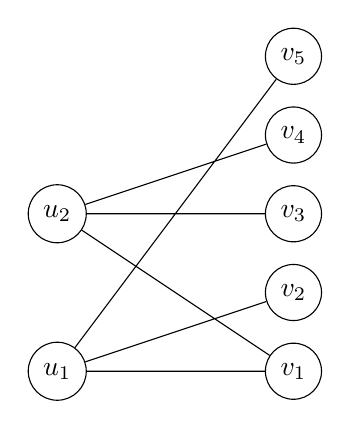
\begin{tikzpicture}%[scale=2.5]
\tikzstyle{every node}=[draw,shape=circle];

\draw node (v0) at (0,1) {$u_1$};
\draw node (v6) at (0,3) {$u_2$};
\draw node foreach \x in {1,2,3,4,5} (v\x) at (3,\x) {$v_\x$};

%\path (0:0cm) node (v0) {$v_0$};
%\path (-36:1cm) node (v1) {$v_1$};
%\path (-2*36:1cm) node (v2) {$v_2$};
%\path (0:1cm) node (v3) {$v_3$};
%\path (36:1cm) node (v4) {$v_4$};
%\path (2*36:1cm) node (v5) {$v_5$};
\draw (v0) -- (v1)
(v0) -- (v2)
(v0) -- (v5)
(v6) -- (v3)
(v6) -- (v4)
(v6) -- (v1);
\end{tikzpicture}
\caption{location.}
    \label{fig:location}
    \end{subfigure} 
  \end{figure}
  \begin{lemma}
    \label{lemma:reduce}
    If the error is at wight less than $\beta n $ then a single round of the  majority reduce the error by at least constant fraction. 
  \end{lemma}
  \begin{proof}
  Denote by $S^{(0)} \subset V^{+}$ and  $T^{(0)} \subset V^{-}$ the subsets of left and right vertices adjacent to the error. And denote by $T^{(1)} \subset T^{(0)}$ the right vertices such any of them is connect by at least $\frac{1}{2}\delta_{0}\Delta$ edges to vertices at $S^{(0))}$. Note that that any vertex in $V^{-}/T^{(1)}$ has on his local view less than $\frac{1}{2}\delta_{0}\Delta$ faulty bits, So it corrects into his right local view in the first right correction round. Therefore after the right correction round the error is set only on $T^{(1)}$'s neighbourhood, namely at size at most $\Delta|T^{(1)}|$.  We will show that this amount is strictly lower by a constant factor than $|e|$. 

  First, let's use the expansion property (\Cref{def:mix}) for getting an upper bound on $T^{(1)}$ size: \begin{equation*}
  \begin{split} 
    \frac{1}{2}\delta_{0}\Delta |T^{(1)}| & \le \Delta \frac{|T^{(1)}||S^{(0)}|}{n} + \lambda\sqrt{|T^{(1)}||S^{(0)}|} \\ 
  \left( \frac{1}{2} \delta_{0} \Delta - \frac{|S^{(0)}|}{n} \Delta \right) |T^{(1)}| & \le \lambda \sqrt{|T^{(1)}||S^{(0)}|} \\ 
|T^{(1)}| & \le \left( \frac{1}{2} \delta_{0} \Delta - \frac{|S^{(0)}|}{n} \Delta \right)^{-2}\lambda^{2} |S^{(0)}| 
  \end{split}
\end{equation*}
Since any left vertex adjoins to at most $\Delta$ faulty bits we have that $\Delta|S^{(0)}| \le |e|$. Combing with the inequality above we get:  

\begin{equation*}
  \begin{split}
    \Delta |T^{(1)}| \le \left( \frac{1}{2} \delta_{0} \Delta - \frac{|e|}{n} \right)^{-2}\lambda^{2} |e|
  \end{split}
\end{equation*}
Hence for $|e|/n \le \beta =  \frac{1}{2} \delta_{0} \Delta - \sqrt{2\lambda}$ it holds that $\Delta|T^{(1)}| \le \frac{1}{2}|e|$. Namely the error is reduced by half.  
\end{proof}

\subsubsection{Pippenger Construction.} The main insight behind Pippenger's construction is that against non trivial noise there is no point in decoding completing back to the code space since it's likely that in the follow turn the block will absorb a magnificent error. So instead of full decoding, one can perform a partial decoding round, for example, a single round of local majority. Keeping reducing the error will ensure that he distance of the state, with hight probability, will remain close (enough) to the ideal state along an ideal computation. 
 
In the original construction, any bit encoded using the repetition code, notice that the repetition code can be thought as expander code on the bipartite $\Delta$-regular graph where the local code $C_{0}$ is the repetition code on $\Delta$ bits. Then one can use \Cref{lemma:reduce} to show that a single round of decoding reduces the error by half.     

Encode any bit of the original code by $n$ bits using the repetition code. Replace any of the AND, and the OR gate by their transversal gates. In each even turn apply a single round of the majority decoder. Finally at the end apply the decoder.  


  \begin{figure}[h]
    \begin{subfigure}[h]{0.05\textwidth}
      \
    \end{subfigure}
    \begin{subfigure}[h]{0.40\textwidth}

  Once again, the feasibility question raised again, this time regarding quantum computing, and while an intensive work has been done, and also succeed to prove that polynomial quantum computation can be made fault tolerance, \cite{aharonov1999faulttolerant},\cite{gottesman2014faulttolerant} and even with only constant overhead at the original circuit width \cite{grospellier:tel-03364419}, the required depth over-head is till not well understood. We stress out that in all the familiar constructions, in construct to Pippenger \cite{Pippenger}, original constant-depth gates are mapped to asymptotically grow\footnote{Note, that here, classical computation is also counted in the overall depth cost} depth gates. 
    \end{subfigure}
    \begin{subfigure}[h]{0.05\textwidth}
      \
    \end{subfigure}
    \begin{subfigure}[h]{0.40\textwidth} 

    %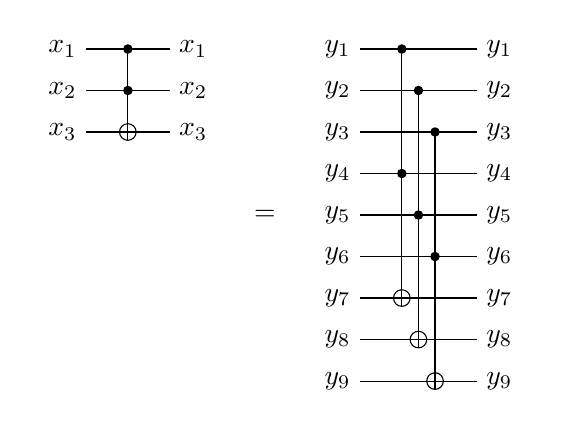
\begin{tikzpicture}[scale=1.000000,x=1pt,y=1pt]
\filldraw[color=white] (0.000000, -7.500000) rectangle (183.000000, 127.500000);
% Drawing wires
% Line 1: x_1 W x_1 x_1 y_1 y_1
\draw[color=black] (13.500000,120.000000) -- (58.500000,120.000000);
\draw[color=black] (112.500000,120.000000) -- (169.500000,120.000000);
% Line 2: x_2 W x_2 x_2 y_2 y_2
\draw[color=black] (13.500000,105.000000) -- (58.500000,105.000000);
\draw[color=black] (112.500000,105.000000) -- (169.500000,105.000000);
% Line 3: x_3 W x_3 x_3 y_3 y_3
\draw[color=black] (13.500000,90.000000) -- (58.500000,90.000000);
\draw[color=black] (112.500000,90.000000) -- (169.500000,90.000000);
% Line 7: y_4 W y_4 y_4
\draw[color=black] (112.500000,75.000000) -- (169.500000,75.000000);
% Line 8: y_5 W y_5 y_5
\draw[color=black] (112.500000,60.000000) -- (169.500000,60.000000);
% Line 9: y_6 W y_6 y_6
\draw[color=black] (112.500000,45.000000) -- (169.500000,45.000000);
% Line 10: y_7 W y_7 y_7
\draw[color=black] (112.500000,30.000000) -- (169.500000,30.000000);
% Line 11: y_8 W y_8 y_8
\draw[color=black] (112.500000,15.000000) -- (169.500000,15.000000);
% Line 12: y_9 W y_9 y_9
\draw[color=black] (112.500000,0.000000) -- (169.500000,0.000000);
% Done with wires; drawing gates
% Line 14: x_1 START
\draw[color=black] (21.000000,120.000000) node[fill=white,left,minimum height=15.000000pt,minimum width=15.000000pt,inner sep=0pt] {\phantom{$x_1$}};
\draw[color=black] (21.000000,120.000000) node[left] {$x_1$};
% Line 15: x_2 START
\draw[color=black] (21.000000,105.000000) node[fill=white,left,minimum height=15.000000pt,minimum width=15.000000pt,inner sep=0pt] {\phantom{$x_2$}};
\draw[color=black] (21.000000,105.000000) node[left] {$x_2$};
% Line 16: x_3 START
\draw[color=black] (21.000000,90.000000) node[fill=white,left,minimum height=15.000000pt,minimum width=15.000000pt,inner sep=0pt] {\phantom{$x_3$}};
\draw[color=black] (21.000000,90.000000) node[left] {$x_3$};
% Line 17: x_1 x_2 +x_3
\draw (36.000000,120.000000) -- (36.000000,90.000000);
\filldraw (36.000000, 120.000000) circle(1.500000pt);
\filldraw (36.000000, 105.000000) circle(1.500000pt);
\begin{scope}
\draw[fill=white] (36.000000, 90.000000) circle(3.000000pt);
\clip (36.000000, 90.000000) circle(3.000000pt);
\draw (33.000000, 90.000000) -- (39.000000, 90.000000);
\draw (36.000000, 87.000000) -- (36.000000, 93.000000);
\end{scope}
% Line 18: x_1 END
\draw[color=black] (51.000000,120.000000) node[fill=white,right,minimum height=15.000000pt,minimum width=15.000000pt,inner sep=0pt] {\phantom{$x_1$}};
\draw[color=black] (51.000000,120.000000) node[right] {$x_1$};
% Line 19: x_2 END
\draw[color=black] (51.000000,105.000000) node[fill=white,right,minimum height=15.000000pt,minimum width=15.000000pt,inner sep=0pt] {\phantom{$x_2$}};
\draw[color=black] (51.000000,105.000000) node[right] {$x_2$};
% Line 20: x_3 END
\draw[color=black] (51.000000,90.000000) node[fill=white,right,minimum height=15.000000pt,minimum width=15.000000pt,inner sep=0pt] {\phantom{$x_3$}};
\draw[color=black] (51.000000,90.000000) node[right] {$x_3$};
% Line 22: =
\draw[fill=white,color=white] (78.000000, -6.000000) rectangle (93.000000, 126.000000);
\draw (85.500000, 60.000000) node {$=$};
% Line 24: x_1 START
\draw[color=black] (120.000000,120.000000) node[fill=white,left,minimum height=15.000000pt,minimum width=15.000000pt,inner sep=0pt] {\phantom{$y_1$}};
\draw[color=black] (120.000000,120.000000) node[left] {$y_1$};
% Line 25: x_2 START
\draw[color=black] (120.000000,105.000000) node[fill=white,left,minimum height=15.000000pt,minimum width=15.000000pt,inner sep=0pt] {\phantom{$y_2$}};
\draw[color=black] (120.000000,105.000000) node[left] {$y_2$};
% Line 26: x_3 START
\draw[color=black] (120.000000,90.000000) node[fill=white,left,minimum height=15.000000pt,minimum width=15.000000pt,inner sep=0pt] {\phantom{$y_3$}};
\draw[color=black] (120.000000,90.000000) node[left] {$y_3$};
% Line 27: y_4 START
\draw[color=black] (120.000000,75.000000) node[fill=white,left,minimum height=15.000000pt,minimum width=15.000000pt,inner sep=0pt] {\phantom{$y_4$}};
\draw[color=black] (120.000000,75.000000) node[left] {$y_4$};
% Line 28: y_5 START
\draw[color=black] (120.000000,60.000000) node[fill=white,left,minimum height=15.000000pt,minimum width=15.000000pt,inner sep=0pt] {\phantom{$y_5$}};
\draw[color=black] (120.000000,60.000000) node[left] {$y_5$};
% Line 29: y_6 START
\draw[color=black] (120.000000,45.000000) node[fill=white,left,minimum height=15.000000pt,minimum width=15.000000pt,inner sep=0pt] {\phantom{$y_6$}};
\draw[color=black] (120.000000,45.000000) node[left] {$y_6$};
% Line 30: y_7 START
\draw[color=black] (120.000000,30.000000) node[fill=white,left,minimum height=15.000000pt,minimum width=15.000000pt,inner sep=0pt] {\phantom{$y_7$}};
\draw[color=black] (120.000000,30.000000) node[left] {$y_7$};
% Line 31: y_8 START
\draw[color=black] (120.000000,15.000000) node[fill=white,left,minimum height=15.000000pt,minimum width=15.000000pt,inner sep=0pt] {\phantom{$y_8$}};
\draw[color=black] (120.000000,15.000000) node[left] {$y_8$};
% Line 32: y_9 START
\draw[color=black] (120.000000,0.000000) node[fill=white,left,minimum height=15.000000pt,minimum width=15.000000pt,inner sep=0pt] {\phantom{$y_9$}};
\draw[color=black] (120.000000,0.000000) node[left] {$y_9$};
% Line 34: x_1 y_4 +y_7
\draw (135.000000,120.000000) -- (135.000000,30.000000);
\filldraw (135.000000, 120.000000) circle(1.500000pt);
\filldraw (135.000000, 75.000000) circle(1.500000pt);
\begin{scope}
\draw[fill=white] (135.000000, 30.000000) circle(3.000000pt);
\clip (135.000000, 30.000000) circle(3.000000pt);
\draw (132.000000, 30.000000) -- (138.000000, 30.000000);
\draw (135.000000, 27.000000) -- (135.000000, 33.000000);
\end{scope}
% Line 35: x_2 y_5 +y_8
\draw (141.000000,105.000000) -- (141.000000,15.000000);
\filldraw (141.000000, 105.000000) circle(1.500000pt);
\filldraw (141.000000, 60.000000) circle(1.500000pt);
\begin{scope}
\draw[fill=white] (141.000000, 15.000000) circle(3.000000pt);
\clip (141.000000, 15.000000) circle(3.000000pt);
\draw (138.000000, 15.000000) -- (144.000000, 15.000000);
\draw (141.000000, 12.000000) -- (141.000000, 18.000000);
\end{scope}
% Line 36: x_3 y_6 +y_9
\draw (147.000000,90.000000) -- (147.000000,0.000000);
\filldraw (147.000000, 90.000000) circle(1.500000pt);
\filldraw (147.000000, 45.000000) circle(1.500000pt);
\begin{scope}
\draw[fill=white] (147.000000, 0.000000) circle(3.000000pt);
\clip (147.000000, 0.000000) circle(3.000000pt);
\draw (144.000000, 0.000000) -- (150.000000, 0.000000);
\draw (147.000000, -3.000000) -- (147.000000, 3.000000);
\end{scope}
% Line 38: x_1 END
\draw[color=black] (162.000000,120.000000) node[fill=white,right,minimum height=15.000000pt,minimum width=15.000000pt,inner sep=0pt] {\phantom{$y_1$}};
\draw[color=black] (162.000000,120.000000) node[right] {$y_1$};
% Line 39: x_2 END
\draw[color=black] (162.000000,105.000000) node[fill=white,right,minimum height=15.000000pt,minimum width=15.000000pt,inner sep=0pt] {\phantom{$y_2$}};
\draw[color=black] (162.000000,105.000000) node[right] {$y_2$};
% Line 40: x_3 END
\draw[color=black] (162.000000,90.000000) node[fill=white,right,minimum height=15.000000pt,minimum width=15.000000pt,inner sep=0pt] {\phantom{$y_3$}};
\draw[color=black] (162.000000,90.000000) node[right] {$y_3$};
% Line 41: y_4 END
\draw[color=black] (162.000000,75.000000) node[fill=white,right,minimum height=15.000000pt,minimum width=15.000000pt,inner sep=0pt] {\phantom{$y_4$}};
\draw[color=black] (162.000000,75.000000) node[right] {$y_4$};
% Line 42: y_5 END
\draw[color=black] (162.000000,60.000000) node[fill=white,right,minimum height=15.000000pt,minimum width=15.000000pt,inner sep=0pt] {\phantom{$y_5$}};
\draw[color=black] (162.000000,60.000000) node[right] {$y_5$};
% Line 43: y_6 END
\draw[color=black] (162.000000,45.000000) node[fill=white,right,minimum height=15.000000pt,minimum width=15.000000pt,inner sep=0pt] {\phantom{$y_6$}};
\draw[color=black] (162.000000,45.000000) node[right] {$y_6$};
% Line 44: y_7 END
\draw[color=black] (162.000000,30.000000) node[fill=white,right,minimum height=15.000000pt,minimum width=15.000000pt,inner sep=0pt] {\phantom{$y_7$}};
\draw[color=black] (162.000000,30.000000) node[right] {$y_7$};
% Line 45: y_8 END
\draw[color=black] (162.000000,15.000000) node[fill=white,right,minimum height=15.000000pt,minimum width=15.000000pt,inner sep=0pt] {\phantom{$y_8$}};
\draw[color=black] (162.000000,15.000000) node[right] {$y_8$};
% Line 46: y_9 END
\draw[color=black] (162.000000,0.000000) node[fill=white,right,minimum height=15.000000pt,minimum width=15.000000pt,inner sep=0pt] {\phantom{$y_9$}};
\draw[color=black] (162.000000,0.000000) node[right] {$y_9$};
% Done with gates; drawing ending labels
% Done with ending labels; drawing cut lines and comments
% Done with comments
\end{tikzpicture}

    \caption{location.}
    \label{fig:location}
    \end{subfigure} 
  \end{figure}



%\begin{definition}
%  \label{def:trig}
%  Let $C$, $\tilde{C}$ be linear binary codes at the same length, We will say that $\tilde{C}$ is a \trig with respect to $C$ if: 
%  \begin{enumerate}
%    \item $\tilde{C} \subset C$
%    \item $|x\cdot y \cdot z|$ is even for $x,y,z \in C$ such that at least one of $x,y,z$  belongs to $\tilde{C}$. 
%    \item $|x\cdot y|$ is even for $x,y \in C$ such that at least one of $x,y$  belongs to $\tilde{C}$. 
%  \end{enumerate}
%  If a code $C$ is \trig with respect to itself then we will say that $C$ is a self \trig code. 
%\end{definition}
%For example, the empty code, that contains only the zero code word, i.e $C = \{ 0 \}$, is a \trig with respect to any code. In fact for proving \Cref{theorem:main} taking the empty code is sufficient. For other example, the \trig codes defined in \cite{bravyi2012magic} are \trig with respect to themself. 

\subsection{Quantum Codes.} \label{sec:quantum} A quantum code over $n$ qubits is an embedding of $\mathcal{H}_{2}^{\otimes k}$ as a subspace of $\mathcal{H}_{2}^{\otimes n}$. Similar to classical codes, we will call $n$ and $k$ the physical and logical qubits. The embeddings of states in $\mathcal{H}_{2}^{\otimes k}$ are called codewords or encoded states. In addition, we will use the term "logical operator" (i.e. logical $X_{i}$) to describe an operator that acts on the code space exactly as it would act on the logical space $\mathcal{H}_{2}^{\otimes k}$ (in our example, turning on and off the encoded state corresponds to the $i$th qubit exactly as $X_{i}$ acts as Pauli $X$ on the $i$th qubit in $\mathcal{H}_{2}^{\otimes k}$). 

We will denote by $X$ and $Z$ the single $X$ and $Z$ Pauli operators, by $X_{i}$ the application of $X$ on the $i$th qubit and nothing else (identity) on the rest of the qubits. By $X^{(v)}$ for some $v \in \mathbb{F}_{2}^{n}$, we mean the operator composed by applying $X$ on each of the qubits whose index is a non-trivial coordinate of $v$ and identity elsewhere. In a similar fashion, we define $Z^{(v)}$. When the context is clear, we will allow ourselves to omit the brackets, i.e. $Z^{v}$. The weight of a Pauli operator is the number of coordinates on which the operator acts non-trivially. Recall that the set of Pauli $+ I$ spans all the Hermitian matrices. We say that the Pauli weight of an operator is the maximal weight of a Pauli in its Pauli decomposition. For example, consider the operator $A = IXX + ZII$, the weight of $A$ is $2$.

The distance of a quantum code is the minimal weight of an operator that takes one codeword to another. We use the standard bracket notation to describe quantum states and in addition, we define for a vector space $A \subset \mathbb{F}_{2}^{n}$ the notation $\ket{A}$ to represent the uniform superposition of all the vectors belonging to that space, namely: \begin{equation*}
  \begin{split}
\ket{A} = \frac{1}{\sqrt{|A|}}\sum_{x \in A}{\ket{x}}
  \end{split}
\end{equation*}
We define in the same way the notation to hold for affine spaces, $\ket{x +A}$. We will use $\propto$ to denote a quantum states up to normalization factor, for example $\ket{\psi} \propto \ket{0} + \ket{1}$ means that $\ket{\psi} = \frac{1}{\sqrt{2}}(\ket{0} + \ket{1})$.
A CSS code is a quantum code defined by a pair of classical codes $C_{X}$ and $C_{Z}$, satisfying $C_{Z}^{\perp} \subset C_{X}$, such that any codeword of it has the form $\ket{x + C_{Z}^\perp}$, where $x \in C_{X}$. We will use $Q$ to refer to a CSS code in general and use $\QQ$ to refer to the vectors associated with the $X$-generators or the encoded states in the computational basis. In the same way, $C_{Z}/C_{X}^{\perp}$ refers to the $Q$ in the phase basis. We will say that a CSS code $Q$ is a LDPC if $C_{X}$ and $C_{Z}$ are both LDPC codes. Our construction uses the classical Tanner code \cite{Tanner}, the expander codes \cite{ExpanderCodes}, and \Hyp  code (quantum expanders) \cite{Leverrier_2015}, \cite{Tillich_2014}, \cite{overheadofquantumerrorcorrection}. We will not describe these constructions and refer the reader to those papers for further information.

\subsection{Decoders.} \label{sec:decoders} We denote by $C_{g}$ the good qLDPC code \cite{Dinur} \cite{Pavel} \cite{leverrier2022quantum}, and by $C_{ft}$ the concatenation code presented at \cite{aharonov1999faulttolerant} ($ft$ stands for fault tolerance). For a code $C_{y}$, we use $\Phi_{y}, E_{y}, D_{y}$ to denote the channel maps circuits into the their matched circuits compute in the code space, the encoder, and the decoder, respectively. We use $\Phi_{U}$ to denote the 'Bell'-state storing the gate $U$. We say that a state $\ket{\psi}$ is at a distance $d$ from a quantum code $C$ if there exists an operator $U$ that sends $\ket{\psi}$ into $C$ such that $U$ is spanned on Paulis with a degree of at most $d$. Sometimes, when the code being used is clear from the context, we will say that a block $B$ of qubits has absorbed at most $d$ noise if the state encoded on $B$ is at a distance of at most $d$ from that code.


\section{Todo:}
\begin{enumerate}
  \item Move to encoding each qubit by logarithmic width (instead of chanks) the reason is that the gate teleportation becomes complicated when it applied over higher dimension. 
  \item Then showing for 2-qubit gates set that is indeed works.
  \item Treating separately to noise observed in two qubits gates. 
\end{enumerate}


\section{ Fault tolerance Toffoli. } 

\ctt{In that section the $\cdot$ operation is the pair wise product (pair wise AND).}

Assume that $\bar{0}, \bar{1} \in C_{X}$ and that they belong to two different cosets of $\QQ$. Let $x,y \in \{ \bar{0},\bar{1}  \}$. 
\begin{equation}
  \label{equation:toff}
  \begin{split}
&    \sum_{z,z^{\prime},w \in \Czdu }{ \ket{z}\ket{z^{\prime}}\ket{w} } \\  
&    \sum_{z,z^{\prime},w \in \Czdu }{ \ket{z}\ket{z^{\prime}}\ket{w + z\cdot z^{\prime}} } \\  
&    \sum_{z,z^{\prime},w \in \Czdu }{ \ket{z + x }\ket{z^{\prime} + y}\ket{w + z\cdot z^{\prime}} } \\  
&    \sum_{z,z^{\prime},w \in \Czdu }{ \ket{z + x }\ket{z^{\prime} + y}\ket{ x\cdot y + x \cdot z^{\prime} + y \cdot z + z z^{\prime} + w + z\cdot z^{\prime}} } \\  
&    \sum_{z,z^{\prime},w \in \Czdu }{ \ket{z + x }\ket{z^{\prime} + y}\ket{ x\cdot y + x \cdot z^{\prime} + y \cdot z +  w } } 
  \end{split}
\end{equation}
Since $x,y \in \{ \bar{0},\bar{1}  \}$ we have that $ x\cdot z^{\prime}$ equals to either $z^{\prime}$ or $\bar{0}$. Hence $ \sum_{w \in \Czdu}{\ket { \xi +x \cdot z + w } } =  \sum_{w \in \Czdu}{\ket { \xi + w } } $. So the idea is the following, suppose that one has to compute Toffoli at time $t$ over the registers $R_{1},R_{2},R_{3}$. First, at time $0$, he initialize a logical zero $\ket{\Czdu}$ in each register, then he compute pairwise Toffoli $R_{1},R_{2}$ into $R_{3}$. That gives the ket $\sum_{z,z^{\prime},w \in \Czdu}{\ket{ z\cdot z^{\prime} + w}}$,  immediately afterwords encode $R_{3}$ again into a good quantum code. Denote by $\tau$ the time required for decoding $R_{3}$ back, at time $t-\tau$ start to decode $R_{3}$. Eventually at time time $t$ compute again the transversal Toffoli, by \Cref{equation:toff} we gets the desired.  


By similar arguments exhibited at \Cref{claim:noisepa} one can show that the errors behaves according to a Pauli noise channel. \ctt{That is not correct, since the concatenation construction assumes that all the registers initialized to physical zeros in the begging of the computation}.

\subsection{Another Idea, $z\cdot z^{\prime}$ cann't contribute too mach.}
Clearly we have that  $|z\cdot z^{\prime}| \le |z|,|z^{\prime}|$ therefore we have that $\prbm{ | z \cdot z^{\prime} | \ge t}{z,z^\prime \in \Czdu} \le \prbm{ | z | \ge t}{z\in \Czdu}$. Now assume that the tanner code by which the code defined is bipartite graph and denote by $z_{+},z_{-}$ the grouping of the $z$'s generators supported on the even and the odd vertices of the graph. By triangle inequality $|z| = |z_{+} + z_{-}| \le |z_{+}| + |z_{-}|$, So if $|z| > t$ then at least one of $|z_{-}|,|z_{+}|$ is greater than $t/2$. Hence via the union  bound: 
\begin{equation*}
  \begin{split}
    \prbm{ |z|  }{z\in \Czdu} \le \prbm{ \bigcup_{i \in \pm }{|z_{i}| \ge t/2}   }{z\in \Czdu} \le \sum_{i \in \pm }{\prbm{ |z_{i}| \ge t/2   }{z\in \Czdu}}
  \end{split}
\end{equation*}

Since any two positive (negative) generators are disjoint we have that  $|z_{+}|$ is a sum of the independent random variables each stands for the weight contributed by a positive vertex. Let us denote by $V^{+}, V^{-}$ the positive and the negative vertices and for each vertex $v \in V$ we will denote by $_{v}$ the bits of $z$ restricted to $v$ edges. So $|z_{\pm}| = \sum_{v \in V^{\pm}}{ |z_{v}| }$. For simplicity assume that $|V^{+}| = |V^{-}| = n/2$ and that $\exppm{|z|}{z \in C_{A}\otimes C_{B}} = \mu $. Then we can use concentration inequality to have: 

\begin{equation*}
  \begin{split}
    \prbm{ |z|  }{z\in \Czdu} \le \sum_{i \in \pm }{\prbm{ \sum_{v \in V^{i}}{ |z_{v}|} \ge t/2   }{z\in \Czdu}} \le 2e^{-(\mu - \frac{t}{2}) n }
  \end{split}
\end{equation*}
Thus if $\mu - \gamma  \ge O (1) $ (from \Cref{claim:error} ) then with high probability the Toffoli is computed up to reducible error.    

\subsection{Using Polynomials Codes.} Consider the CSS code above $\mathbb{F}_{q}$ defined by the stabilizers $C_{Z}^{\perp} = \braket{\{ x^{2i} : i\ge \frac{1}{2}d - c \}}$ and $C_{X}^{\perp} = \braket{\{ x^{2i+1} : i \ge \frac{1}{2}d - c \}}$ for some $c = O(1)$. Clearly the $X$-stabilizers commute with the $Z$-stabilizers. 



\section{ The Noise Model } 
Informally classical noisy circuits describe the running computation of circuits when the bits have probabilities to flip. As exactly to the classical case, in noisy quantum circuits qubits have probabilities to fault. We formalise the noise model by defining a channel $\mathcal{N} : \mathcal{C} \rightarrow \mathcal{D}\left(\mathcal{C}\right)$ that given an ideal circuit induce distribution over circuits. For example, one can consider a Pauli channel, which  after each gate of the original circuit, either do nothing with probability $1-p$ or, with probability $1-p$ impose uniformly one of the Pauli operators $X,Z,Y$. Formally:  
\begin{definition}
  Pauli channel $\mathcal{N}: \mathcal{C}\rightarrow \mathcal{D} \left( \mathcal{C} \right)$ defined to give on input $C \in \mathcal{C}$ the distribution over circuits $\tilde{C}$ where any even location of $(i, 2j)$ of $\tilde{C}$ equals to the $(i,j)$ location of $C$, and any odd location $(i,2j+1)$ of $\tilde{C}$ is the density operator $(1-p) I + \frac{p}{3} \left(X + Y + Z  \right)$. 
\end{definition}

The Pauli channel is charactered by exhibits an independent noise on the qubits, Yet for most of the fault tolerance construction a much more weaker property is required to be assumed. We say that a channel is a local stochastic noise channel if the probability to error to be occur is exponentially decays at the number of qubits the error supports.  
 
\begin{definition}
  An error channel $\mathcal{N}: \mathcal{C}\rightarrow \mathcal{D} \left( \mathcal{C} \right)$ will be said to be a local stochastic noise channel if there exists a constant $c$ such the probability to a fault to be applied on locations $(I ,j)$, where $I$ is a subset of qubits, is less than $c^{-n}$.
\end{definition}

Another important property of a noise model which we consider in this work is the accessibility to fresh qubits, also known as resets gate. When having an access to fresh qubits one can assume that in any time in the computation there are qubits at the $\ket{0}$ states. Usually those qubits are used to measured the syndrome relative to an error correction code. It was proven that without an access to fresh qubits quantum circuits cannot last than logarithmic depth without mixing into a fully mixed state, meaning to be turned into complete garbage \cite{aharonov1996limitationsnoisyreversiblecomputation}. That result also holds for a classical noisy computation. 

\begin{definition}
  An error channel $\mathcal{N}: \mathcal{C}\rightarrow \mathcal{D} \left( \mathcal{C} \right)$ will be said to has a fresh qubits access if location $(i,j)$ in an output gate $\tilde{C}$ has a non zero probability to exhibits a fault if there is a $j^{\prime} < j$ such a location $(i, j^{\prime})$ such that on the input circuit $C$, at location $(i,j^{\prime})$ a non identity gate is posed.     
\end{definition}

We close this section by formalize the \noiseQNCon class. 
\begin{definition}
  We denote by \noiseQNCon the class of decision problems solvable by logarithmic-depth quantum circuits, subjected to a local stochastic noise,  with bounded probability of error. 
\end{definition}
We mention that in \cite{aharonov1996limitationsnoisyreversiblecomputation}, it was proved how a fault tolerance circuit with an access to fresh qubits, at logarithmic depth, can be converted to a log depth circuits without a fresh qubits access at the cost which is at most polynomial in wide. Meaning that Proving that $ \QNCon \subset $ \noiseQNCon implies also that $ \QNCon $ can be computed, in the presence of noise without an access to fresh qubits. 

\section{ Fault Tolerance (With Resets gates) at Linear Depth. } 

\begin{claim}
There exists a value $p_{th} \in (0,1)$ such that if $p < p_{th}$, then any quantum circuit $C$ with a depth of $D$ and a width of $W$ can be computed by a $p$-noisy circuit $C^{\prime}$, which allows for resets. The depth of $C^{\prime}$ is at most $\max{ \{O(D), O(\log(WD)) \} }$.
\end{claim}


\subsection{Initializing Magic for Teleportation gates and encodes ancillaries.}
The Protocol: \begin{enumerate}
  \item Initialization of zeros: The qubits are divided into blocks of size $|B|$. Each block is encoded in $C_{g}$ using $D_{ft} \Phi_{ft}[E_{g}] \ket{0^{|B|}}$.
  \item Initialization of Magic for Teleportation gates: The gates in the original circuit are encoded in $C_{g}$ using $D_{ft} \Phi_{ft}[E_{g}] \ket{\Phi_{U}}$.
  \item Gate teleportation: Each gate in the original circuit is replaced by a gate teleportation.
  \item Error reduction: After the initialization step, at each time tick, each block runs a single round of error reduction.
\end{enumerate}

\begin{claim}[From \cite{leverrier2022decodingquantumtannercodes}]
  \label{claim:error} 
  Assuming that an error $|e| \le \gamma n $, i.e $e$ is supported on less than $\gamma n$ bits, then a single correction round reduce $e$ to an error $e^\prime$ such that $|e^{\prime}| < \nu |e|$. 
\end{claim}
 %Recall that by definition, $D_{i}E_{i} = I$, or in other words, $D_{i}= E_{i}^{\dagger}$.  
\begin{claim}
  \label{claim:noisepa}
  The gate $ D_{ft} \Phi_{ft}[E_{g}]$ initializes states encoded in $C_{g}$ subject to a $3p$-noise channel.  
\end{claim}
\begin{proof}
  Clearly, with high probability, $\Phi_{ft}[E_{g}]$ successfully encodes into $C_{ft} \circ C_{g}$, let's say with probability $1 - \frac{1}{poly(n)}$. Denote by $E_{i}$ and $D_{i}$ the encoder and decoder at the $i$th level of the concatenation construction. Consider the decoder under $\mathcal{N}$ action: $P_{2}D_{1}P_{2}D_{2},..,P_{i-1}D_{i}P_{i}$, by the fault-tolerance construction, a logical error at the $i$th stage occurs with probability $p^{2^{i}}$. Therefore, by the union bound, the probability that in one of the steps the circuit absorbs an error that is not corrected is less than $p + p^{2} + p^{4} + .. < 2p$. Hence, any decoded qubit absorbs noise with probability less than $2p$.


  Thus, overall, we can bound the probability of a single qubit being faulty by:
  \begin{equation*}
    \begin{split}
      \prb{\text{fault} } &=  \prb{\text{fault} |  \Phi_{ft}[E_{g}] }\cdot \prb{\Phi_{ft}[E_{g}]} + \prb{\text{fault} | \overline{\Phi_{ft}[E_{g}]} }\cdot \prb{\overline{\Phi_{ft}[E_{g}]}}\\
      &\le  \prb{\text{fault} |  \Phi_{ft}[E_{g}] } + \prb{\overline{\Phi_{ft}[E_{g}]}} \le 2p + \frac{1}{poly(n)} \le 3p
    \end{split}
  \end{equation*}

  \begin{remark}
In our construction, we use the concatenation code to encode blocks of length $\log(n)$. Therefore, any $poly(n)$ in the above should be replaced by $\log(n)$. However, this does not affect anything since the inequality does not depend on $n$.
  \end{remark}

%
%
%  \begin{equation*}
%    \begin{split}
%      \mathcal{N}(D) &= \left((\mathcal{N}(D))^{\dagger}\right)^{\dagger} =  \left(\sum_{P_{1}, P_{2}, .., P_{i} \in \mathcal{P}}{ \prb{P_{1}, P_{2}, .., P_{i}}  \left(D_{1}P_{2}D_{2},..,P_{i-1}D_{i}P_{i}\right)^{\dagger}} \right)^{\dagger} \\ 
%      &= \left( \sum_{P_{1}, P_{2}, .., P_{i} \in \mathcal{P}}{ \prb{P_{1}, P_{2}, .., P_{i}}  P_{i}E_{i}P_{i-1}E_{i-1},..,P_{1}E_{1} } \right)^{\dagger}\\
%      &= \left( \left( 1 -\frac{1}{poly(n)} \right)\sum_{P_{i} \in \mathcal{P}}\prb{P_{i}}P_{i}E + \frac{1}{poly(n)} A  \right)^{\dagger} \\ 
%      &= \left( 1 -\frac{1}{poly(n)} \right)\sum_{P_{i} \in \mathcal{P}}\prb{P_{i}}DP_{i} + \frac{1}{poly(n)} A 
%\end{split}
%  \end{equation*}
%
%  %Since $D$ is semi-transversal gate, it preserves the 
%
%
%  And notice that $\star$ is with probability $1 - \frac{1}{poly(n)}$ equals to $E_{i}E_{i-1}..,E_{1}=E$. Hence $\mathcal{N}(D)$ equals to $\left( P E \right)^{\dagger} = PD$.
%
%  \begin{equation*}
%    \begin{split}
%      \braket{ \psi^{\prime} | P_{i}E_{i}P_{i-1}E_{i-1},..,P_{1}E_{1} \psi } = \braket{ \psi^{\prime} P_{i}D_{i}P_{i-1}D_{i-1},..,P_{1}D_{1} | \psi }
%    \end{split}
%  \end{equation*}
%  Thus for any pauli-channel $\mathcal{N} : L(H) \rightarrow L(H)$, and $\psi^{\prime}$ which is a codeword we get: 
%  \begin{equation*}
%    \begin{split}
%      \braket{ \psi^{\prime} \mathcal{N}(D) | \psi } &=  \sum_{P_{1}, P_{2}, .., P_{i} \in \mathcal{P}}{ \prb{P_{1}, P_{2}, .., P_{i}}  \braket{ \psi^{\prime} P_{i}D_{i}P_{i-1}D_{i-1},..,P_{1}D_{1} | \psi }} \\
%      &=  \sum_{P_{1}, P_{2}, .., P_{i} \in \mathcal{P}^{\star}}{  \prb{P_{1}, P_{2}, .., P_{i}}\braket{ \psi^{\prime} | P_{i}E_{i}P_{i-1}E_{i-1},..,P_{1}E_{1} \psi }} \pm O(  \frac{1}{poly(n)})\\
%      &=  \sum_{P_{1}, P_{2}, .., P_{i} \in \mathcal{P}^{\star}}{  \prb{P_{1}, P_{2}, .., P_{i}}\braket{ \psi^{\prime} | P_{i} E \psi }} \pm O(  \frac{1}{poly(n)})\\
%      &\le  \sum_{ P_{i} \in \mathcal{P}}{  \prb{ P_{i}}\braket{ \psi^{\prime} | P_{i} E \psi }} \pm O(  \frac{1}{poly(n)}) \\
%      &\le  \sum_{ P_{i} \in \mathcal{P}^{\le d}}{  \prb{ P_{i}}\braket{ \psi^{\prime} | P_{i} E \psi }} \pm O (e^{-d \cdot n} ) \pm O(  \frac{1}{poly(n)}) \\
%      & \le   \sum_{ P_{i} \in \mathcal{P}/\mathcal{P}^{\star}}{  \prb{ P_{j} \in B_{d}\left( P_{i} \right)}\braket{ \psi^{\prime} | P_{i} E \psi }}  \pm O (e^{-d \cdot n} ) \pm O(  \frac{1}{poly(n)}) 
%    \end{split}
%  \end{equation*}
%  Using the fact that the concatenation code is monotonic (\Cref{def:mono}) we get that the probability to have physical fault $P_{j}$.   
%%\end{widetext}
\end{proof}

\begin{claim}
  \label{claim:prob}
  With a probability $ 1 - \frac{WD}{|B|} \cdot D 2e^{-2|B|(\beta - p)} $, the total amount of noise absorbed in a block at any given time $t$, is less than $\gamma n$. 
\end{claim}
\begin{proof}
Consider the $i$th block, denoted by $B_{i}$. By applying Hoeffding's inequality, we have that the probability that more than $\beta |B|$ qubits are flipped at time $t$ is less than $2e^{-2|B|(\beta - p)}$. By using the union bound over all blocks at all time locations, we can conclude that with probability $1 - \frac{WD}{|B|} \cdot D 2e^{-2|B|(\beta - p)}$, the noise absorbed in a block is less than $|\beta|B$ for the entire computation.

Let $X_{t}$ denote the support size of the error over $B_{i}$ at time $t$. Using \Cref{claim:error}, we can bound the total amount of error absorbed by a block until time $t$ as follows:
\begin{equation*}
\begin{split}
X_{t} \le \nu \cdot (X_{t-1} + \beta |B| ) \le \nu(\gamma+\beta) |B| \le \gamma |B|
\end{split}
\end{equation*}
\end{proof}


\begin{claim}
  The total depth of the circuit is $O ( D  ) + O ( \log^{c} |B| )$. 
\end{claim}
\begin{proof}
  The gate for encoding $|B|$-length blocks in $C_{g}$ is a Clifford gate and can therefore be computed in $O(\log|B|)$ depth. The encoding of the magic/bell states is done by first computing them in the logical space (un-encoded qubits) and then encode them using the encoder. Hence, the fault-tolerant version of both initializing ancillaries and magic states/bell states costs $O( (\log |B|) \cdot \log^{c}( |B| \log |B| ) )$ \footnote{The width of the original circuit is $|B|^{2}$ so the number of locations is $ |B|^{2} \cdot \log |B|$} depth \cite{aharonov1999faulttolerant}. Backing into $C_{g}$ from $C_{ft}$ by decoding the concatenation code takes exactly as long as the encoding, namely $O( (\log |B|) \cdot \log^{c}( |B| \log |B| ) )$.

  Then, using the bell measurements, any of the logical gates takes $O(1)$ depth. Since we only perform a single round of error correction, the remaining computation until the last decoding stage takes at most constant time of the original depth. Finally, we pay $O(\log |B|)$ for complete decoding. Summing all, we get: 
  \begin{equation*}
    \begin{split}
     &  O ( \log |B|\cdot  \log^{c}( |B| \log |B| ) )  + O ( D  ) + O ( \log |B| ) \\ 
     = & O ( D  ) + O ( \log^{c} |B| )
    \end{split}
  \end{equation*}
\end{proof}

Assuming that $W$ is polynomial in $D$, taking the block length to be $|B| = \log((W \cdot D)^c)$, as shown in \Cref{claim:prob}, results in a linear fault tolerance construction with a success probability of $1 - \frac{1}{\log^{c_2}(W \cdot D)}$. This means that the fault tolerance version of circuits in $\textbf{QNC}_1$ has a logarithmic depth. Additionally, using the construction in \cite{aharonov1996limitationsnoisyreversiblecomputation} produces a polynomial fault tolerance circuit in the reversible gates setting. \ctt{ We missed the fact that it requires non trivial classical computation to compute what gate should be applied after the gate teleportation (i.e $UPU^{\dagger}$ )}.



\section{ Does $\NCon \subset $\noiseQNCon ?}


\section{ Does Factoring $\subset$ \noiseQNCon ?}

\begin{equation*}
  \begin{split}
    D(n) &= \Theta(\log n ) + D(\sqrt{n})\\
    \Rightarrow D(n) & = \Theta( \log n ) 
  \end{split}
\end{equation*}



%\section{Current Status.}

\begin{enumerate}
  \item Section 5 - Correct. In any CSS code, one can find a large subspace
    $\Lambda \subset C_{X}$ with a dimension that is linear in $n$ and this
    subspace also satisfies the required relation for distillation.
    Specifically,
    for any $x \in \Lambda$, $y, z \in C_{X}$, it holds that $xy = 0$ and $xyz =
    0$.
  \item Sections 6 and 7 - Incorrect. Initially, I believed that assuming the
    code is LDPC, one could encode the state $C_{Z}^{\perp}$ in constant depth.
    However, this idea turned out to be incorrect both in calculation and in
    contrast to the fact that synthesizing the ground state of the Toric code
    requires $\Omega(\log n)$ depth.
\end{enumerate}

\section{Classic Codes With Few Checks.}

\begin{claim}
  There is a family of classic binary codes, with positive rate,
  $\Theta(n^{\frac{1}{3}})$ distance, and $\gamma n^{\frac{1}{3}}$ checks.
\end{claim}
\begin{proof}
  We are going to show the existences of bipartite expander, over $n$ left
  vertices and $\gamma n^{\frac{1}{3}}$ right vertices such that for any $S
  \subset L $ at size at most $\alpha n^{\frac{1}{3}}$, the neighbors of $S$ is
  at size at least $\beta|S|$. We use the standard probabilistic 'fusion
  construction', meaning that we are going to sample permutation from $ [n
  \times  d_{1}]$ to $[n^{\frac{1}{3}} \times d_{2}]$ and fuse together
  $d_{1}$'s left vertices subsets $\{ d_{1} \cdot j,  d_{1} \cdot j + 1, d_{1}
  \cdot j + 2, .. ,d_{1} \cdot (j+1) -1 \}$ and similarly fuse together $d_{2}$
  right vertices.

  Now observes that the probability of neighbors $S \subset L$ being contained
  in $T \subset R$  is at most:
  \begin{equation*}
    \begin{split}
      \prb{X_{S,T}} \le \frac{ |T|d_{2} \cdot ( |T|d_{2} -1) \cdot \cdot \cdot
      ( |T|d_{2} -|S| d_{1})}{ nd_{1} \cdot ( nd_{1} -1) \cdot \cdot \cdot  (
      nd_{1}- |S|d_{1})} \le \left( \frac{|T|d_{2}}{ nd_{1}- |S|d_{1}   }
      \right)^{|S|d_{1}}
    \end{split}
  \end{equation*}
  And for the $|T| <\beta |S|$ the above is lower than:
  \begin{equation*}
    \begin{split}
      \prb{X_{S,T}} \le \left( \frac{2\beta|S|d_{2}}{ nd_{1}  }
      \right)^{|S|d_{1}}
    \end{split}
  \end{equation*}

  By the union bound we get that the probability that there exist $S$ at size
  $|S| < \alpha n^{\frac{1}{3}}$ such that the neighbors of $S$ is at size less
  than $\beta|S|$ is bounded by:
  \begin{equation*}
    \begin{split}
      \prb{\bigcup_{\substack{ |S| < \alpha n^{\frac{1}{3}} \\ |T| < \beta |S|
      }} X_{S,T} }  & \le \sum_{\substack{ |S| < \alpha n^{\frac{1}{3}} \\ |T| <
      \beta |S|  }}{ \prb{X_{S,T}}  } \\
      & \le \sum_{k\ge 1}^{\alpha n^{\frac{1}{3}}}{  { n \choose k  }{ \gamma
        n^{\frac{1}{3}} \choose \beta k  }\cdot \left( \frac{2\beta kd_{2}}{
          nd_{1}  }
      \right)^{kd_{1}}} \\
      & \le \sum_{k\ge 1}^{\alpha n^{\frac{1}{3}}}\left( \frac{e^{2+\beta}}{k}
        \cdot \frac{n^{1+\beta/3}}{\beta^{\beta}k^{\beta}} \cdot \left(
          \frac{2\beta
      kd_{2}}{n d_{1}} \right)^{d_{1}} \right)^{k} \\
      & = \sum_{kge 1}^{\alpha n^{\frac{1}{3}}}\left( \frac{e^{2+\beta}}{k}
        \cdot \frac{n^{1+\beta/3}}{\beta^{\beta}k^{\beta}} \cdot \left(
          \frac{2\beta k
      n^{2/3}d_{1}}{n d_{1}} \right)^{d_{1}} \right)^{k} \\
      & =  \sum_{k\ge 1}^{\alpha n^{\frac{1}{3}}}\left( \frac{e^{2+\beta}
        (2\beta)^{d_{1}} }{\beta^{\beta}} \cdot \frac{k^{d_{1}- \beta - 1
      }}{n^{d_{1}/3 - \beta/3 - 1}}  \right)^{k} \\
      & \le  \sum_{k\ge 1}^{ \infty }\left( \frac{e^{2+\beta} (2\beta)^{d_{1}}
        }{\beta^{\beta}} \cdot \gamma^{d_{1}- \beta/3 - \frac{1}{3} }
      \right)^{k} =
      \frac{1}{\varepsilon} - 1
    \end{split}
  \end{equation*}
  So one can find parameters such that the probability is strictly less than
  $1$ meaning that with positive probability we sample our desirable bipartite
  expander graph.


\end{proof}

The idea form here, set $C_{Z}$ to be the above code, and $C_{X}^{\perp} =
\emptyset  $, clearly $C_{X}^{\perp} \subset C_{Z}$. Now, construct $\Lambda$
by the method in section 6.The additional phase that we get by applying the
gate $T^{n}$ corresponds to controlled-S, controlled-controlled-Z between the
generators of $C_{Z}^{\perp}$. So one can fix them by applying at most
$\Theta( (\gamma n^{\frac{1}{3}})^{3})$ perfect $T$ gates. In total, if we
show a decoder that against noise $p$ susses to correct with probability $q$,
Then we got a distillation protocol that consume $\gamma^{3}n$ perfect magic
states, $n$ noisy magic states at error rate $p$ and with probability $q$
distillate $\rho n$ magic states.
\begin{equation*}
  \begin{split}
    \braket{ \gamma^{3} n, n, p } \rightarrow \braket{0, \rho n, q}
  \end{split}
\end{equation*}

\section{Bipartite Random Constructions, Collisions Number.}

Let $u,v\in R$ be checks vertices (right vertices) and let $Y_{u,v}$ the
indicator for a bit been ceheckd by both $u$ and $v$ checks, Means that there
is a left vertex $w$ adjances to both $u,v$.

\begin{equation*}
  \begin{split}
    \prb{Y_{u,v} = 0  | N(v)} & \ge \frac{ \left( nd_{1} - d_{2}d_{1} \right)
      \left( nd_{1} - d_{2}d_{1} - 1 \right)\cdot\cdot\cdot\left( nd_{1} -
    d_{2}d_{1} - d_{2}  \right)   }{ nd_{1} \cdot \left( nd_{1} - 1 \right)
    \cdot\cdot\cdot \left( nd_{1} - d_{2} \right)  }  \\
    & = \prod_{i \in d_{2}}{ 1 - \frac{d_2d_1}{nd_1 - i} }\ge  \left( 1 -
    \frac{d_2d_1}{nd_1 - d_{2}} \right)^{d_2} \ge 1  - d_{2}\frac{d_2d_1}{nd_1 -
    d_{2}}\\
    & \ge 1 - 2\frac{d_{2}^{2}}{n}
  \end{split}
\end{equation*}

\ifdefined\DETAILS
\begin{equation*}
  \begin{split}
    \prb{Y_{u,v} = 0 } = \sum_{N(v)}{\prb{Y_{u,v} = 0 | N(v) } \cdot
    \prb{N(v)}} \ge  1 - \frac{d_{2}^{2}}{2n}
  \end{split}
\end{equation*}
\fi

Thus, the excpection for collision between $u$ and $v$ and expected total
collisions number are less than:
\begin{equation*}
  \begin{split}
    \expp{Y_{u,v}} &\le 2\frac{d_{2}^{2}}{n}\\
    \expp{\sum_{u,v \in R}Y_{u,v}} &\le { n\frac{d_1}{d_2} \choose 2 }
    2\frac{d_{2}^{2}}{n} \le nd_1^{2}\\
    & \sim n \cdot { d_{1} \choose 2 } \sim m d_{2}d_{1}
  \end{split}
\end{equation*}

Another direction, assume that we choose the adjacency matrix by picking
function such that the probablilty of overlapping is $\sim \frac{\gamma}{n}$.
And then:

\begin{equation*}
  \begin{split}
    \expp{Y} \sim m^{2} \cdot \frac{\gamma}{n} = \frac{d_{1}}{d_{2}} m\gamma =
    \left( \frac{d_1}{d_2} \right)^{2}\gamma n
  \end{split}
\end{equation*}
So, for any 'subset' of $m$ edges use another hash function, (first labaling
$R$ with random labels, and then draw $h \sim \mathcal{H}$). The probability
for collision, by the union bound is lower than $ d_2 \cdot \frac{1}{n}$.
Therfore if we take $d_2$ to behave like $\sim  d_{1}^{5}$, then:

\begin{equation*}
  \begin{split}
    \expp{Y} \sim  \left( \frac{d_1}{d_2} \right)^{2}\gamma n \sim   \left(
    \frac{d_1}{d_2} \right)^{2} d_2 n = \frac{n}{d_{1}^{3}}
  \end{split}
\end{equation*}

\section{Decoding The Code.}

Consider the simplest decoding procedure, any right vertex in $R$ decode it's
local view using decoder $D$. The probability of failure is lower than the
probability that there is a single vertex which fails to decode.

\begin{equation*}
  \begin{split}
    \prb{\text{failure}} & \le \prb{\ \exists v \in R \text{  which fails to
    decode }} \\
    & \le m \cdot \prb{ |e(\Gamma(v))| \ge \mu  }\le  m \cdot \prb{
    |e(\Gamma(v))| \ge (1 + \theta) p d_{2} } \\
    & \le m \cdot e^{-\frac{\theta^{2}}{2+\theta} d_{2}p}
  \end{split}
\end{equation*}

%\section{ Punctured Polyonomial Codes. }
%
%
%
%
%\ifdefined\DETAILS
%$ \varphi : x \mapsto \left(x \right)^{i} \mod \Delta$ act as isomorphisem on
% $\mathbb{F}_{\Delta}$.
%\fi
%
%\begin{equation*}
%\begin{split}
%\sum_{\substack{ x \in \mathbb{F}_{\Delta} \\ x < \Delta  }}{ x^{i+j}}
% =_{\Delta}  \sum_{ x \in \mathbb{F}_{\Delta} }{ x^{i+j}}
% =_{\Delta}\begin{cases}  0  & i + j\neq_{q} \Delta - 1 \\
%\Delta - 1 & \text{else}
%\end{cases}
%\end{split}
%\end{equation*}
%
%So the punctured $d$-dgree polynomial code is orthogonal for the punctured
% $n-1-d$ polyonimal code. So we can take $d = q/2 - 1$, and $\Delta = \alpha
% q$ to have $[\alpha q, q/2 -1, q/2 - (1-\alpha)q]$ code. For example we can
% take $\alpha = 7/8$ and have   $[7/8 q, q/2 -1, 3/8 q]$. The rate of the code
% is
%\begin{equation*}
%\begin{split}
%\sim \frac{1}{2} / \frac{7}{8} = \frac{4}{7} > \frac{1}{2}
%\end{split}
%\end{equation*}
%
%\begin{claim}
%For any $\Delta > 5$ there are good LDPC family $C$ such that for any $x,y \in
% C$ it holds that $x\cdot y=_{(\Delta-1)} 0$.
%\end{claim}
%\begin{proof}
%Consider the Tanner code defined by using the $\Delta$-punctured polynomial
% code as $C_{0}$, where the rate of $C_{0}$ is strictly greater than
% $\frac{1}{2}$. Then we have for any $x,y\in C$:
%\begin{equation*}
%\begin{split}
%x\cdot y =_{(\Delta-1)} \sum_{v\in V^{+}}{x|_{v} \ \cdot  \ y|_{v}}
% =_{(\Delta-1)} 0
%\end{split}
%\end{equation*}
%\end{proof}
%
\section{Candidate For Triorthogonal LDPC Code.}

\begin{claim}
  Consider the ring $\mathbb{F}_{q}[x]$ where $q$ is a prime number. Let
  $\Delta = 4^{c}$ where $c \ge 3$. Then we have:
  \begin{equation*}
    \begin{split}
      \sum_{x \in [\Delta]}{x^{i}} =_{\Delta} \in \{  0  \ , \ \Delta/2  \}
    \end{split}
  \end{equation*}
\end{claim}
\begin{proof}
  By induction on $c$.
  \begin{enumerate}
    \item Base. For $c = 3$ we computes the summation bruthforcely.
    \item Assumption. Assume the correctness of the claim for $c-1$.
    \item Step. Denote by $B_{j}(\Delta)$ the bucket $\Delta\cdot j +1,
      \Delta\cdot j +2, .. \Delta \cdot (j+1)-1$. Observes that:
      \begin{equation*}
        \begin{split}
          \sum_{x\in B_{j+1}(\Delta)}{x^{i}} =_{\Delta}\sum_{x\in
          B_{j+1}(\Delta)}{(x-\Delta)^{i}} =_{\Delta} \sum_{x\in
          B_{j}(\Delta)}{x^{i}}
        \end{split}
      \end{equation*} On the other hand, by the induction assumption, there is
      some integer $a$ for which:
      \begin{equation*}
        \begin{split}
          \sum_{x\in B_1(\Delta/4)}{ x^{i} } = \Delta/8 \cdot a
        \end{split}
      \end{equation*}
      Thus the summation over $\Delta$ elements equals to:
      \begin{equation*}
        \begin{split}
          \sum_{x \in [\Delta]}{x^{i}} = \sum_{j \in [4]}\sum_{x \in
          B_{j}(\Delta/4)}{x^{i}} =  \Delta/8 \cdot a \cdot 4 = \Delta \cdot a
          /2
        \end{split}
      \end{equation*}
  \end{enumerate}
\end{proof}

\begin{definition}
  Let $G =(L,R, E)$ be a bipartite graph, and let $\Delta$ be an integer.
  Define $G^{\prime}$ to be the graph:  $G^{\prime} = (\Delta \times L, R,
  E^{\prime})$ defined as follows:
  \begin{equation*}
    \begin{split}
      E^{\prime} = \{  \{ (i,v), u \} : i\in [\Delta], \{u,v\} \in E \}
    \end{split}
  \end{equation*}
  In addition, we define the equivalence relation $u\sim v$ for $u,v \in \Delta
  \times L$ to hold if the first coordinates of $u$ and $v$ are equal.
\end{definition}

Let $G^{\prime}$ be a graph constructed as described above. Consider the code
$C$  over the $\mathbb{F}_{q}$ alphabet, defined as all the assignments of
symbols from $\mathbb{F}_{q}$ to the $\Delta \times L$ vertices. Such any
vertex on the right side of $G$ sees a polynomial of degree at most $d$ on its
local view, in addition the $x$'s value of bit in $\Delta \times  L$ is the
same module $\Delta$ for all the checks.
To clarify, if one checks, treat $u\in \Delta \times L$ as the value of the
polynomial at coordinate $z$, and treat the other check as the value of the
polynomial at coordinate $z^{\prime}$, then $z =_{\Delta} z^{\prime}$.

\begin{claim}
  $C$ is a good LDPC code. (If $G$ is expander graph).
\end{claim}

\begin{proof}
  We obtain a lower bound on the code dimension by subtracting restrictions. So,
  \begin{equation*}
    \begin{split}
      \dim C = \Delta \cdot |L| - |R| \cdot(1-\rho) \cdot q
    \end{split}
  \end{equation*}
  Now, assume trough contradiction that there is $x \in C$ at weight $|x|
  <\gamma n$ denote by $S^{\prime} \subset \Delta \times  L$ the set of vertices
  setted to a non-trivial symbol. And observes that in the original graph $G$,
  $S^{\prime}$ induce a set of vertices $S$  by taking the delegations of the
  equivalence classes.

  Since $G$ is a $(n,m,\gamma,\alpha)$ expander, and $|S| < |S^{\prime}| <
  \gamma n$, it followees that $|\Gamma(S)| > \alpha |S| \Rightarrow $

  \begin{equation*}
    \begin{split}
      & |S| / |\Gamma(S)| <  \frac{1}{\alpha}  \\
      \Rightarrow & |S^{\prime}| / | \Gamma(S)| < \frac{\Delta}{\alpha}
    \end{split}
  \end{equation*}
  So there is a check that sees a local view at weight less than
  $\frac{\Delta}{\alpha}$ bits. (Otherwise,  $|S^\prime| > |\Gamma(S)| \cdot
  \frac{\Delta}{\alpha}$). So, if $\frac{\Delta}{\alpha}$ is lower than $C_{0}$
  distance we get a contradiction.
\end{proof}

\begin{claim}
  Let $h_{1},h_{2},h_{3}$ be arbitrary checks of $C$, not necessarily
  different. Then:
  \begin{equation*}
    \begin{split}
      h_{1}h_{2} &=_{4} 0 \\
      h_{1}h_{2}h_{3} & =_{4} 0
    \end{split}
  \end{equation*}
\end{claim}
\begin{proof}
  Complete it.
\end{proof}

Consider the Tanner \textbf{Graph}, such that the graph $G$ is bipartite, and
every two checks overlap on the $i$th bucket, $\Delta$-size, bits. So for any
two checks, we have that
\begin{equation*}
  \begin{split}
    \sum_{x = i \cdot \Delta }^{(i+1)\Delta}{ x^{j} } &=_{\Delta}
    \sum_{x^{\prime} = (i-1) \cdot \Delta }^{i\Delta}{ (x^{\prime}+\Delta)^{j}
    } \\
    & =_{\Delta} \sum_{x = (i-1) \cdot \Delta }^{i\Delta}{ x^{\prime,j} }
    =\sum_{ x \in \mathbb{F}_{\Delta} }{ x^{j}} \\
    & \ \  \sum_{x \in \mathbb{F}_{\Delta}}{ ( x+a\Delta)^{i}(x + b\Delta)^{j}}
    =\sum_{x\in \mathbb{F}_{\Delta}}{x^{i+j}}
  \end{split}
\end{equation*}
So it's left to show that if we take the bipartite graph to be an expander
graph then we have a good code.

Let $G$ be a bipartite graph $G=(L,R,E)$ that is a $(n,m,\gamma,\alpha)$
expander. This means that for any subset $S \subset V(G)$ with $|S| < \gamma
n$, the size of the group of neighbors of $S$ is at least $\Gamma(|S|) >
\alpha |S|$. Consider the graph $G^{\prime} = (\Delta \times L, R,
E^{\prime})$ defined as follows:
\begin{equation*}
  \begin{split}
    E^{\prime} = \{  \{ (i,v), u \} : i\in [\Delta], \{u,v\} \in E \}
  \end{split}
\end{equation*}
Thus for any $S \subset \Delta \times L$ if $|S|/\Delta < \gamma n$ we have
that: $\Gamma^{\prime}(S) <\Gamma(|S|/\Delta)$.

Therefore, if $S$ is the set of vertices associated with the non-trivial
symbols induced by the assignment of a codeword on the vertices, then if $|S|
< \gamma n$, we have:
\begin{equation*}
  \begin{split}
    \frac{|S|}{\Gamma^{\prime}(|S|)} & \le \frac{|S|}{\Gamma(|S|/\Delta)} \le
    \frac{\Delta}{\alpha}
  \end{split}
\end{equation*}
So there is a check that sees on his local view less than $\Delta/\alpha$
non-trival bits $<d(C_{0})$.

\section{Hyperproduct Code of two Triorthogonal Codes.}

Suppose that $H$ is a parity check matrix scuh that $h_{i}h_{j} =_{\Delta} \in
\{\Delta , \ , \ \Delta/2 \}$ for any two rows. IS that true that the same
property holds for the following check matrix?
\begin{equation*}
  \begin{split}
    H^{\prime} \leftarrow [ H \otimes I | I \otimes H ]
  \end{split}
\end{equation*}

\begin{equation*}
  \begin{split}
    H^{\prime}_{i}H^{\prime}_{j} &= \overbrace{ (H\otimes I)_{i}(H\otimes
    I)_{j}}^{A} + \overbrace{(I \otimes H)_{i}(I \otimes H)_{j}}^{B}
  \end{split}
\end{equation*}
Denote $i = (i_{1},i_{2})$ and $j = (j_{1},j_{2})$. So:
\begin{equation*}
  \begin{split}
    (H\otimes I)_{i}(H\otimes I)_{j} &= \delta_{i_{2},j_{2}} H_{i_{1}}H_{j_{1}}
  \end{split}
\end{equation*}
and
\begin{equation*}
  \begin{split}
    (I \otimes H)_{i}(I \otimes H)_{j} &= \delta_{i_{1},j_{1}}
    H_{i_{2}}H_{j_{2}}
  \end{split}
\end{equation*}
So $H^{\prime}_{i}H^{\prime}_{j}$ can only be nonzero if the corresponding rows
multiplication of either $A$ or $B$ is nonzero. Thus the number of no
commuting checks is less than  $2n\cdot\gamma n = 2\gamma n^{2}$. Hence it is
statisfied to require that $\gamma \le \sqrt{\frac{\rho}{2}}$ for having
positive balance ( $2\gamma n^{2} < k^{2} $).

\section{The Balacne Equation.}
Assume for the momment that indeed one has to pay only $\gamma n < k $ of
non-clifford gates in the pre-encoding stage. What exactly is given by that?
\begin{equation*}
  \begin{split}
    T(\rho n) = \overbrace{\gamma n}^{\text{ perfect }} +\overbrace{n}^{\text{
    noisy }}
  \end{split}
\end{equation*}

Let's assume also that we found a good LDPC family such the above assumption
holds and that the decoder can by using only Clifford gates and messurments
correct any error at size less than $\Theta(n)=\tilde{d}n$. Then the protocol
extands into:

\begin{equation*}
  \begin{split}
    T(\rho n) =
    \begin{cases}
      \overbrace{\gamma n}^{\text{ perfect }} +\overbrace{n}^{\text{ noisy }}
      & \text{ w.p }  1 - p^{\tildeP{d}n}  \\
      \text{junk} & \text{else}
    \end{cases}
  \end{split}
\end{equation*}

Now, Let $T^{\prime}$ be the distillation protocol that uses a subroutine
protocol for quaderic redunecy, and sums up to balacne equation $n \mapsto
\rho^{\prime} n$, at cost of $\gamma n$ perfect magic states. Can we realx it
somehow? Think about using the uinon bound on the $\gamma n$ near to perfect
states.

For generating the $\gamma n$ pefrect states, we will have to call reqursivly,
to ask for $\gamma n \frac{\gamma}{\rho}$ states. If the probability for
failure for each use of nearly perfect magic state is less than $q$ then the
probability of general failutre is less than:
\begin{equation*}
  \begin{split}
    & \gamma n \cdot \sum q(i) \left( \frac{\gamma}{\rho} \right)^{i} \le  q
    \cdot \frac{\gamma n }{ 1 - \frac{\gamma}{\rho}}
  \end{split}
\end{equation*}

\begin{equation*}
  \begin{split}
    T(\rho n, q_{0}) & = \overbrace{T(\gamma n, q_{1})}^{\text{nearly perfect
    }} +\overbrace{n}^{\text{ noisy }}   \\
    T(\rho n, q_{0}) &= T(n, \sqrt{q}) + T(\gamma n, \sim \frac{1}{n})
  \end{split}
\end{equation*}

Suppose that we have a machine that produce with probability $\frac{1}{2}$ $k$
magic states with error rate $\sim \frac{1}{2^{n}}$. Does that machine useful?
Noitce that for obtaing such high accuricite one has to pay overhead of
$n\cdot n^{\beta}$ width. Here we reduce it to be:
\begin{equation*}
  \begin{split}
    \sum^{\log \log 2^n}{ \left(\frac{\gamma}{\rho}\right)^{i} n  \log^{\beta}
    \left( n \right)} = n \log^{\beta} n \cdot O(1)
  \end{split}
\end{equation*}
So in excpection the number of magic states that one might consume is double
the above amount.

\begin{equation*}
  \begin{split}
    & p^{c^{i_{0}}}+ p^{c^{i_{0}+1}}+ p^{c^{i_{0}+2}} + ... + p^{\tilde{d}
    n}\le  p^{c^{i_{0}}}+ p^{2c^{i_{0}}}+ p^{3c^{i_{0}}} + ... \\
    \le \  & p^{c^{i_{0}}} \cdot \frac{1}{1 - p^{c^{i_{0}}}}
  \end{split}
\end{equation*}

[IDEA] For fault tolerance theorems, one can start by distillate $n^{\alpha}$
magic states by the non-linear techniques, at error rate  $< 2^{\sqrt{n}}$, So
the time complexity for the initial distillation is sub-linear in $n$. And
then start the above Such that $p^{c^{i_{0}}} \sim
p^{\delta^{\prime}n^{\alpha}}$.

\section{Hyper Lift Preserves Few-Overllaps.}

Assume that  $G^{(i)}$ is a bipartite such that for any two right vertices pair
either they don't have a common neighbor or they have exactly one common
neighbor. Denote by $\gamma^{(i)}$ the relative number of overlapped checks
and similarly by $\gamma^{(i+1)}$ the that ratio in respect to $G^i{(i+1)}$,
the graph which obtained from $G^{(i)}$ by lifting. Then $\gamma^{(i)} =
\gamma^{(i+1)}$.

\section{ What about the $Z$-product? }
$Z$-product, there is an edge between $u$ and $v$ if there is blue-red-blue
path between them. First notice that bipartite graph remains bipartite.
Second, if $u$ and $v$ belongs to two different sources, and there is also
edge between $u$ to $v^{\prime}$. If $v$ and $v^{\prime}$ came form the same
source. Then $v$ and $v^{\prime}$ share $d-1$ on their support, they use the
same first blue and red edges, and only the last one change. Meaning that if
$d$ is odd, then, we don't obtain new uncommute checks. Now lets assume that
$v$ and $v^{\prime}$ come from different sources. So how many from $u$ cloud
is belongs for both of them. Meaning that now we take two different red edges.
So take a vertex on the input set (left vertex). Now, for reach both $v$ and
$v^{\prime}$ it has to be one of $V_{0}/{x,y}$. Means that we have multiply by
$d-2$.

What about triple? Sp any one of $d-3$ doesn't encounter at all. And then we
remain only with the impact of disjoints pairs. That might helps. If we assume
that no triple has been instrected before, then we remains static with the
portion. If the expansion get's worse by only constant factor then we can
increase logratimic number of time.

\section{The problem with the above.}
The code that is obtained by the polynomial tanner is (almost) self dual code,
module $\Delta$ the multiplication $x \cdot x$ belongs to $\{ 0, \Delta/2 \}$.
While what we actually want to have is $x \cdot x =_{4} 1$. An idea how to
correct that, sets the checks such only two of them don't commute. After
taking the Hyprproduct code, they will turned to $\Theta(\sqrt{n})$ that don't
commute. So if we have a perfect $\Theta(\sqrt{n})$ T states, we can cancel
their phase before the encoding.

Let $B$ be the bucket which matches $\{2,3,..\Delta-1\}$. On that bucket, the
multiplication of the checks corresponds to $\sum_{x\in
\mathbb{F}_{\Delta}}x^{i} - 1^i$, which is $\in \{ -1, \Delta/2 - 1 \}$. On
the otherhand, the codeword $\xi$ that corresponds to the constant function
$f(x)= 1$ in every bucket gives $\xi \cdot \xi =_{\Delta} -1$.

So $\xi^{\prime} = \xi \otimes I$ padding with zeros, is a codeword of the
Hyprproduct code, such that $\xi^{\prime}\cdot \xi^{\prime} = 1$.

\section{Good Codes With Large $\Lambda$.}
\newcommand*{\DETAILS}{}
\ifdefined\DETAILS

\fi

\begin{claim}
  \label{claim:find}
  Let $v_{1},v_{2}..v_{k}$ vectors in $\mathbb{F}_{2}^{n}$, then there are
  $u_{1},u_{2}..u_{k^{\prime}}$ for $k^{\prime} > k/2$. Such $\text{ span } \{
  u_{1},u_{2}..u_{k^{\prime}} \} \subset \text{ span } \{ v_{1},v_{2}..v_{k} \}$
  and for any $i,j$ it holds that $u_{i}u_{j} = 0$.
\end{claim}

\begin{figure}[h]
  \label{fig:fig1}
  \begin{subfigure}[b]{0.45\textwidth}
    \label{fig:fig2}
    \begin{algorithm}[H]
      \caption{ Find commuted vectors $u_{1}, u_{2}, .. u_{k^{\prime}}$  }
      \label[algorithm]{alg:pick}
      Let $ J \leftarrow \emptyset$ \\
      \For{$i \in [k/2]$}{
        $J \leftarrow J \cup \{v_{2i-1}, v_{2i}\}$ \\
        \For{ $S \subset J$ }{
          Compute the vector $m_{S}$ \\
          \ \ \ define as $m_{S,j} = u_{j} \sum_{w\in S}w$
        }
        Pick $S$ such $m_{S} = 0$ and set $u_{i} \leftarrow  \sum_{w\in S}w$ \\
        Choose randomly $w \in S$ and set $J \leftarrow J/w$
      }
    \end{algorithm}
  \end{subfigure}
  \begin{subfigure}[b]{0.05\textwidth}
    \
  \end{subfigure}
  \begin{subfigure}[b]{0.45\textwidth}
    \begin{algorithm}[H]
      \caption{ Find commuted vectors $u_{1}, u_{2}, .. u_{k^{\prime}}$  }
      \label{alg:picktrip}
      Let $ J \leftarrow \emptyset$ \\
      \For{$i \in [k/3]$}{
        $J \leftarrow J \cup \{v_{3i-2}, v_{3i-1}, v_{3i}\}$ \\
        \For{ $S \subset J$ }{
          Compute the vector $m_{S}$ \\
          \ \ \ define as $m_{S,j,j^{\prime}} = u_{j^{\prime}} u_{j} \sum_{w\in
          S}w$
        }
        Pick $S$ such $m_{S} = 0$ and set $u_{i} \leftarrow  \sum_{w\in S}w$ \\
        Choose randomly $w \in S$ and set $J \leftarrow J/w$
      }
    \end{algorithm}

  \end{subfigure}
\end{figure}


\begin{proof}
  Consider \Cref{alg:pick}, We are going to prove that at line number (8) the
  alg always finds a subset $S$ that satisfies the equality.  Assume not. On one
  hand, the number of possible values that $m_{S}$ can have is $2^{i} - 1$. On
  the other hand, since $J$ contains $i+1$ vectors on the $i$th iteration, it
  follows that the number of subsets is $ 2^{i+1}-1 \ge 2^{i}$.

  Therefore, there must be at least two different subsets $S$ and $S^{\prime}$
  such that $u_{S}=u_{S^{\prime}}$. However, this means that
  \begin{equation*}
    \begin{split}
      m_{S\Delta S^{\prime}, j} &= u_{j} \sum_{w\in S\Delta S^{\prime}}w =
      u_{j}\left(  \sum_{w\in S\Delta S^{\prime}}w + 2 \sum_{w \in S\cap
      S^{\prime}}w\right) \\
      & = m_{S,j} +m_{S^{\prime},j} = 0
    \end{split}
  \end{equation*}
  Thus, $m_{S\Delta S^{\prime}} = 0$. Additionally, it is clear that the rank
  does not decrease, as for $u_{i}$, there exists one $v_{j}$ such that only
  $u_{i}$ is supported by $v_{j}$.
\end{proof}

\begin{claim}
  Let $v_{1},v_{2}..v_{k}$ vectors in $\mathbb{F}_{2}^{n}$ and $m$ be an integer
  $m<k$, then there are $u_{1},u_{2}..u_{k^{\prime}}$ for $k^{\prime} > k/2-m$.
  Such $\text{ span } \{   u_{1},u_{2}..u_{k^{\prime}} \} \subset \text{ span }
  \{ v_{m+1},v_{m+2}..v_{k} \}$, for any $i,j$ it holds that $u_{i}u_{j} = 0$
and for any $i\in ]k^{\prime}$, $j\le m$ it holds that $u_{i}v_{j} = 0$.
\end{claim}
\begin{proof}
  Modify the \Cref{alg:pick} as follows, Initialize $u_{1},.u_{m}$ to be
  $v_{1},..,v_{m}$ and $J = \{v_{m+1},..v_{2m+2}\}$. Notice that in the $i$th
  iteration, for the counting argument to works in the proof of
  \Cref{claim:find}, we have to ensure that:
  \begin{equation*}
    \begin{split}
      |J| \ge &  m+i+1 \text{,  So  } m+i+1\le k - m - i  \\
      \Rightarrow & i \le k/2 -m - \frac{1}{2}
    \end{split}
  \end{equation*}
  In the end, $u_{m+1},u_{m+2},..,u_{k^{\prime}}$ will satisfy the equations.
\end{proof}
\begin{claim}
  Let $v_{1},v_{2}..v_{k}$ vectors in $\mathbb{F}_{2}^{n}$, then there are
  $u_{1},u_{2}..u_{k^{\prime}}$ for $k^{\prime} > k/4$. Such $\text{ span } \{
  u_{1},u_{2}..u_{k^{\prime}} \} \subset \text{ span } \{ v_{1},v_{2}..v_{k}
  \}$. And for any $i,j$ $\sum u_{i,k}u_{j,k} =_{4} 0$.
\end{claim}
\begin{proof}
  Use the \Cref{alg:pick} twice. However, in the second iteration, define
  $m_{S,j}$ to be the product of module 4. Note that $m_{S,j}$ must be either
  $4n$ or $4n+2$. Thus, we can follow the proof of \Cref{claim:find}.
\end{proof}

\begin{claim}
  \ctt{Complete for the above the version, which handle triples.} number of
  options is $\left(2^{i}\right)^2 = 2^{2i}$ and therefore we have the
  correctness if $|J| > 2i+1$.
\end{claim}

\begin{claim}
  Consider the Left-Right ($\Delta$,$n$)-Complex $\Gamma$. $\dim
  C_{X}/C_{Z}^{\perp} \cap C_{Z} / C_{X}^{\perp}$ is linear in $n$.
\end{claim}
\begin{proof}
  The rates of both $C_{X}/C_{Z}^{\perp}$ and $C_{Z}^{\perp}/C_{X}^{\perp}$ are
  $(2\rho-1)^{2}$, where $\rho$ can be any number in the range $(0,1)$
  \cite{leverrier2022quantum}. Consider choosing $\rho$ such that the rates of
  the quotient spaces are strictly greater than $\frac{1}{2} + \alpha$. This
  implies that the rate of their intersection is greater than $2\alpha$.
\end{proof}
\begin{corollary}
  Fix the rate of the small codes $C_{A}$ and $C_{B}$ to $\rho = \frac{1}{2} +
  \alpha$.  There is a subspace $\Lambda \subset C_{X}/C_{Z}^{\perp}$ at rate
  $\frac{1}{4} \cdot  2\alpha$ such that for any $x \in \Lambda$ and $y,z \in
  C_{Z}^{\perp} \cup \Lambda$ it holds that: %$xy =_{2} 0$ and also for any $x,y
  % \in \Lambda$ $x,y =_{4} 0$.
  \begin{enumerate}
    \item $xy =_4 0 $
    \item $xyz =_4 \sum_{i}x_{i}y_{i}z_{i} =_4  0$
  \end{enumerate}
\end{corollary}

\ifdefined\MORE
\begin{claim}
  \label{claim:commute}
  Let $C$ be a $[n,k,d]$ binary linear code, and let $\Lambda$ be subcode
  $\Lambda \subset C$ at dimension $k' > \alpha k$ for some $\alpha\in(0,1)$.
  Then there exists a code $C' = [\leq 2n, \geq (1 - \alpha +
  \frac{\alpha^{3}}{24})k, d]$ and a subcode of it $\Lambda' $ in it at
  dimension $\ge \frac{\alpha^{3}}{24}k$, such:
  \begin{enumerate}
      \label{property:prop}
    \item For every $x \in \Lambda'$ and $y \in C^{\prime} \ \ x\cdot y = 0$
    \item For every $x \in \Lambda'$ and $y,z \in C^{\prime} \ \ x \cdot y
      \cdot z =0 $
  \end{enumerate}
\end{claim}
\begin{proof}
  First, we can assume that the generator matrix of $C$ is an upper triangular
  matrix, such that the first $k^\prime$ rows span $\Lambda$. Notice that after
  applying the algorithm from \Cref{claim:stair} starting from the first row and
  stopping at the $k^{\prime}$th row, the first $k^{\prime}$ rows are kept in
  $\Lambda$. So let's assume that is the form of the generator matrix.


  Now, let's consider the following process: going uphill, from right to left,
  starting at the $k^\prime$ row. Initially, set $j \leftarrow k^{\prime}$ and
  in each iteration, advance it to be the index of the next row, namely
  $j\leftarrow j - 1$. In each iteration, ask how many rows $G_{m}$, such that
  $m \le j$, satisfy $G_{m} G_{j} = 0$ and how many pairs of rows
  $G_{m},G_{m^{\prime}}$ such that $m,m^{\prime}\le j$ satisfy $G_{m}\cdot
  G_{m^{\prime}} \cdot G_{j} = 0$. Denote by $p$ the probability to fall on
  unsatisfied equation from the above.
  \begin{itemize}
    \item If $p \ge \frac{1}{2}$ then we move on to the next iteration.
    \item Otherwise, we encode the $j$th coordinate by $C_{0}$, which maps $1
      \rightarrow w$ such that $w\cdot w = 0$. This flips the value of $G_{m}
      G_{j}$
      for any pair and $G_{m} G_{m^{\prime}} G_{j}$ for any triple such that
      $m,m^{\prime} \le j$, so we get that the majority of the equations are
      satisfied. Also notice that the concatenation doesn't change the value of
      any
      multiplication at the form $G_{m}G_{j^{\prime}}$ for $j^{\prime}> j$.
      Therefore, for any $j< j^{\prime}\le k^{\prime}$ the number of the
      satisfied
      equations relative to $j^{\prime}$ is not changed, meaning it is still the
      majority.

      Set $G$ to be the new matrix after the concatenation by $C_{0}$.
  \end{itemize}

  In the end of the process $G$ is going to be the generator matrix of
  $C^{\prime}$. It's left to construct $\Lambda^{\prime}$, we are going to do so
  by taking from the $k^{\prime}$ rows a subset that satisfies the desired
  property in \Cref{property:prop}.

  Let $S$ be the set of rows among the first $k^{\prime}$ rows for which there
  is at least one unsatisfied equation. We will now prove that if $k^{\prime}$
  is large enough, specifically linear in $k$, then $|S|$ is small enough to
  obtain $\Lambda^{\prime}$ by removing the rows in $S$.

  Observe that the number of satisfied equations is at least:
  \begin{equation*}
    \begin{split}
      & \frac{1}{2}\left(k^{\prime}-1+(k^{\prime}-1)^{2}\right)
      +\frac{1}{2}\left(k^{\prime}-1+(k^{\prime}-1)^{2}\right)
      +\frac{1}{2}\left(k^{\prime}-2+(k^{\prime}-2)^{2}\right)  + ..
      +\frac{1}{2}\left(1+( 1 )^{2}\right) \\
      & = \frac{1}{2} \left(  { k^{\prime} + 1 \choose 2 }  +
      \frac{k^{\prime}(k^{\prime}+1)(2k^{\prime}+1)}{6} \right)
    \end{split}
  \end{equation*}
  So
  \begin{equation*}
    \begin{split}
      |S| \cdot k + |S|\cdot k^{2}  & \le  k^{\prime} \left( k + k^{2} \right)
      - \frac{1}{2} \left(  { k^{\prime} + 1 \choose 2 }  +
      \frac{k^{\prime}(k^{\prime}+1)(2k^{\prime}+1)}{6} \right)
      \\
      \Rightarrow & |S| < k^{\prime} - \frac{1}{2}\left( \frac{1}{k^{2}+k} {
        k^{\prime} + 1 \choose 2 }  + \frac{1}{k^{2}+k}
      \frac{k^{\prime}(k^{\prime}+1)(2k^{\prime}+1)}{6} \right) \\
      \Rightarrow & |S| < k^{\prime} - \frac{k^{\prime 3}}{24k^{2}} <k^{\prime}
      - \alpha^{2}\frac{k^{\prime} k^{2}}{24k^{2}}
    \end{split}
  \end{equation*}

  Therefore, if $k^{\prime} \ge  \alpha k$ we have that $|S| < (1
  -\frac{\alpha^{2}}{24})k^{\prime}$ implies that $\dim \Lambda^{\prime} \ge
  \frac{\alpha^{3}}{24} k$.

\end{proof}
\fi

\begin{claim}
  Consider $C,\Lambda$ and $C^{\prime},\Lambda^{\prime}$ defined in
  \Cref{claim:commute}. Denote by $\bar{\Lambda}$ the subspace $C/\Lambda$.
  Then:
  \begin{equation*}
    \begin{split}
      d(C^{\prime}/\bar{\Lambda^{\prime}}) \ge d( C/\bar{\Lambda })
    \end{split}
  \end{equation*}
\end{claim}

\begin{proof}
  The way we perform Guess elimination is critical. We want to make sure that
  we do not add an $\Lambda$ row to a $\bar{\Lambda}$ row. \ctt{Continue, Easy.
    Just need to perform the row reduction when rows of $\Lambda$ at bottom, and
  then rotate the matrix $  \curvearrowright $    }
  \begin{equation*}
    \begin{split}
      \begin{bmatrix}
        A & B \\
        C & D
      \end{bmatrix}  \curvearrowright
      \begin{bmatrix}
        D & C \\
        B & A
      \end{bmatrix}
    \end{split}
  \end{equation*}
\end{proof}

\begin{claim}[Not Formal]
  It is easy to see that by using concatenation again, one can obtain the code
  $\dim \Lambda^{\prime} \leftarrow \frac{1}{2}\dim \Lambda^{\prime}$. For any
  $x \in \text{ gen } \Lambda^{\prime}$, $|x|_{4} = 1$, and for any $x \in
  C^{\prime} / \Lambda^{\prime}$, we have $|x|_{4} = 0$.
\end{claim}

\begin{proof}
  \ctt{
    We will do it by iterating the generators of $C$ after performing rows
    reduction to the generator matrix. Now we will concatenate the $i$
    coordinate
    to complete the weight of the $i$th row to satisfy the requirements.
  }
\end{proof}

\section{Compute $\ket{C_{Z}^{\perp}}$ In Constant Depth. \ctt{Wrong Section.}}
Let $C_{0}$ be a $\Delta$-length error linear binary code, $\Gamma$ a
$\Delta$-regular bipartite graph, and let $C_{Z}$ be the Tanner code defined
by $C_{0}$ and $\Gamma$. We are about to prove that the uniform superposition
over $C_{Z}^\perp$ codewords can be computed with constant probability at a
depth dependent only on $\Delta$, in particular independent of the
$C_{Z}^{\perp}$-length. For this, we are going to use Proposition 10 in
\cite{moore1998parallel}, which states that both the encoder and the decoder
of any stabilizer $m$-length code can be implemented by a circuit at depth
$\Theta(\log m)$ with $\Theta(m^{2})$ ancillae.

\begin{claim}
  Let $G$ be a $\Delta$-regular bipartite graph, and denote by $C_{Z}^{\perp}$
  the dual-tanner code $\mathcal{T}(G,C^{\perp}_{0})^\perp$. Then there is a
  circuit that with constant probability computes the state
  $\ket{C_{Z}^{\perp}}$ at $\Theta(\log \Delta)$ depth, and
  $\Theta(\Delta^{2})n$ ancillary qubits.
  %Suppose that $G_{}
\end{claim}

\begin{proof}
  Let $E_{v}$ and $D_{v}$ be the encoder and the decoder of $C_{0}$ over the
  local view of vertex $v$, By \cite{moore1998parallel} we have that both have
  depth $\Theta(\log \Delta)$ and require $\Delta^{2}$ ancillae.
  Since $\Gamma$ is bipartite, we can decompose $V$ into $V^{-}$ and $V^{+}$
  such that the local views of any two vertices in $V^{\pm}$ are disjoint.
  Therefore, for any two different vertices $v,u \in V^{\pm}$, the encoders
  $E_v$ and $E_u$ act on disjoint subsets of qubits, each corresponding to the
  local view of either $v$ or $u$. Consider the following algorithm:

  \begin{algorithm}
    \caption{ Compute $\ket{C_{Z}^{\perp}}$ }
    \label{alg:computeCZ}
    Initialize $2n$ qubits. \\
    Call the left and right segments $L$ and $R$. \\
    Apply $E_{v}$ in parallel on $L$ for any $v \in V^{+}$. \\
    Apply $E_{v}$ in parallel on $R$ for any $v \in V^{-}$. \\
    XOR $R$ into $L$ by applying CNOT from the $i$th bit of $R$ to the $i$th
    bit of $L$. \\
    Apply $D_{v}$ in parallel on $R$ for any $v \in V^{-}$. \\
    Apply $H^{k}$ on $L$. And measure. \\
    Accept if the result in $C_{Z}$
  \end{algorithm}

  For any $v \in V$, let $\ket{z_{v}}$ be the superposition of codewords in
  $C_{0}$ supported by the local view of $v$. Similarly, for any subset of
  vertices $W \subset V$, let $\ket{z_{W}}$ be the uniform superposition over
  the subspace spanned by the generators supported by the vertices in $W$. In
  other words:
  \begin{equation*}
    \begin{split}
      \ket{z_{W}} = \ket{\sum_{v \in W} z_{v}}
    \end{split}
  \end{equation*}
  Using the notation, applying the encoders $E_{v},E_{u}$ for any pair of
  vertices with disjoints local view become:
  \begin{equation*}
    \begin{split}
      E_{v}\cup E_{u}\ket{0}^{n} & = E_{v}\ket{0 + z_{u}} = E_{v}\ket{0_{/ u
      \text{'s view }}} \ \otimes \ \ket{ z_{u} } \\
      & = \ket{z_{v}}\ket{z_{u}} = \ket{z_{u} + z_{v}} = \ket{z_{\{ u,v\}}}
    \end{split}
  \end{equation*}
  So applying all the encoders $E_{v}$ at once over the positive vertices
  results in:
  \begin{equation*}
    \begin{split}
      \left(\cup_{v \in V^{+}}E_{v}\right)\ket{0}^{n} =  \left(\cup_{v \in
      V^{+} / v_{0} }E_{v}\right)\ket{z_{v_{0}} + 0} = \ket{z_{V^{+}}}
    \end{split}
  \end{equation*}
  Thus the whole computation sum up into:
  \begin{align*}
    \left(\cup_{v \in V^{+}}E_{v}\right) \otimes \left( \cup_{v \in
    V^{+}}E_{v}\right) & \ & \ket{0}^{n} \otimes \ket{0}^n & \mapsto \\
    \text{CNOT} & \sum_{z \in A}\sum_{z^{\prime} \in B} &\ket{z_{V^{+}}}
    \ket{z_{V^{-}}} & \mapsto  \\
    I \otimes H^{k}  & \sum_{z \in A}\sum_{z^{\prime} \in B} & \ket{z +
    z^{\prime} } \ket{z^{\prime}} & \mapsto  \\
    & \sum_{z \in A}\sum_{z^{\prime} \in B} & \ket{z + z^{\prime} }
    (-1)^{wz^{\prime}} \ket{w } & \mapsto
  \end{align*}
  So if $w \in C_{Z}$ then clearly $z^{\prime}w = 0$. The probability for that
  to occur is
  \begin{equation*}
    \begin{split}
      \prb{w \in C_{Z}} = \frac{|C_{Z}|}{\mathbb{F}_{2}^{n}} = 2^{(\rho-1)n}
    \end{split}
  \end{equation*}

\end{proof}

\section{Distillate $\ket{ \Lambda + C_{Z}^{\perp}}$ Into Magic.}
Let $\ket{f}$ be a codeword in $C_{X}$, and let $\hat{X}_{g}$ be the indicator
that equals $1$ if $f$ has support on generator $g$, and $0$ otherwise.
Observe that applying $T^{\otimes}$ on $\ket{f}$ yields the state:
\begin{equation*}
  \begin{split}
    T^{\otimes n}\ket{f} & =  T^{\otimes n}\ket{\sum_{g} \hat{X}_{g}g } = \exp
    \Big( i\pi/4 \sum_{g} \hat{X}_{g}|g|  -  2 \cdot i \pi/4 \sum_{g,h}
      \hat{X}_{g}\hat{X}_{h}|g\cdot h| \\
      & +  4 \cdot i\pi/4 \sum_{g,h} \hat{X}_{g}\hat{X}_{h}\hat{X}_{l}|g\cdot h
    \cdot l| -   8  \cdot i\pi/4 \cdot \text{ integers } \Big) \ket{f} \\
    & = \exp \Big( i\pi/4 \sum_{g} \hat{X}_{g}|g|  -  2 \cdot \pi/4 \sum_{g,h}
      \hat{X}_{g}\hat{X}_{h}|g\cdot h| +  4 \cdot i\pi/4 \sum_{g,h}
    \hat{X}_{g}\hat{X}_{h}\hat{X}_{l}|g\cdot h \cdot l| \Big) \ket{f}
  \end{split}
\end{equation*}

So in our case:
\begin{equation*}
  \begin{split}
    T^{\otimes n}\ket{f} & = \\
    & = \exp \Big( i\pi/4 \sum_{g \in \text{ gen }\Lambda } \hat{X}_{g}  \\
      \ifdefined\MORECALC & -  2 \cdot \pi/4 \sum_{g \in \text{ gen }\Lambda
      ,h} 2 \hat{X}_{g}\hat{X}_{h} \\ \fi
      & -  2 \cdot \pi/4 \sum_{g ,h \in \text{ gen } C_{Z}^{\perp}}
      \hat{X}_{g}\hat{X}_{h}|g\cdot h| \\
      \ifdefined\MORECALC & +  \cancel{4 \cdot i\pi/4 \sum_{g \in \Lambda ,h}
      \hat{X}_{g}\hat{X}_{h}\hat{X}_{l}2} \\ \fi
      & +  4 \cdot i\pi/4 \sum_{g,h \in \text{ gen } C_{Z}^{\perp}}
    \hat{X}_{g}\hat{X}_{h}\hat{X}_{l}|g\cdot h \cdot l|  \Big) \ket{f}
  \end{split}
\end{equation*}

So eventually, we have a product of gates when non-Clifford gates are applied
on only on generators of $C_{Z}^{\perp}$.
\begin{equation*}
  \begin{split}
    T^{n}\ket{f} = \prod_{g \in \text{ gen }\Lambda} T_{g}
    \ \ \ifdefined\MORECALC \prod_{g \in \text{ gen }\Lambda, h} \{ CZ_{g,h} | I
    \} \ \ \fi \prod_{g ,h \in \text{ gen }C_{Z}^{\perp}} \{ CS_{g,h} |
      CZ_{g,h} |
    I \} \ \ \prod_{g ,h, l \in \text{ gen }C_{Z}^{\perp}} \{ CCZ_{g,h,l} | I \}
    \ket{f}
  \end{split}
\end{equation*}
Decompose $f = f_{1} + f_{2}$, where $f_{1}$ is supported only on
$C_{X}/C^{\perp}_{Z}$ and $f_{2}$ is supported only on $C_{Z}^{\perp}$. By
using commuting relations, the above can be turned into.
\begin{equation*}
  \begin{split}
    T^{n}\ket{f} = & \ifdefined\MORECALC \prod_{g \in \text{ gen }\Lambda, h}
    \{ CZ_{g,h} | I \} \fi \ \ \prod_{g \in \text{ gen }\Lambda} T_{g} \ \
    X_{f_{1}} \\
    &  \ \ \prod_{g ,h \in \text{ gen }C_{Z}^{\perp}} \{ CS_{g,h} | CZ_{g,h} |
    I \} \ \ \prod_{g ,h, l \in \text{ gen }C_{Z}^{\perp}} \{ CCZ_{g,h,l} | I \}
    \ket{f_2}
  \end{split}
\end{equation*}

Denote by $M_1, M_2$ the gates:

\begin{equation*}
  \begin{split}
    M_{1} &= \prod_{g \in \text{ gen } \Lambda, h} \{ CZ_{g,h} | I \} \\
    M_{2} &= \prod_{g ,h \in \text{ gen } C_{Z}^{\perp}} \{ CS_{g,h} | CZ_{g,h}
    | I \} \ \ \prod_{g ,h, l \in \text{ gen } C_{Z}^{\perp}} \{ CCZ_{g,h,l} |
    I \}
  \end{split}
\end{equation*}

And then we get that
\begin{equation*}
  \begin{split}
    \prod_{g \in \text{ gen } \Lambda} T_{g} \ket{f} &=  M_{1}^{\dagger} T^{n}
    M_{2}^{\dagger} \ket{f} \\
    \prod_{g \in \text{ gen }\Lambda} T_{g}\ket{f} &=  M_{1}^{\dagger} T^{n}
    \ \ E \ \ L[M_{2}^{\dagger}] \ \ \ket{L[f]}
  \end{split}
\end{equation*}

\begin{claim}
  Let $v \in V^{-}$, and let $g_{1}$ be the generator supported by $v$, which
  matches an assignment of a codeword in $C_{A}\otimes C_{B}$ on the local view
  of $v$. Denote by $U_{v, g_{1}}$ the control-gate which, depending on the
  control bit $(v,1)$, turns on $g_{1}$ over the edges associated with the local
  view of $v$ in the graph $G$. Then, the depth of $U_{v,g_{1}}$ depend only on
  $\Delta$.
\end{claim}

\begin{claim}
  Let $(v,g_{1})$ and $(u,g_{2})$ be control wires for two different generators
  in the graph $G$. Then $U_{v,g_{1}}$ and $U_{u,g_{2}}$ \ctt{There must be a
    claim about the relationship between two different generators intersection,
  But I don't sure exactly why}.
\end{claim}

\begin{definition}
  We say that a quantum circuit $\mathcal{C}$ is well error spreading if the
  light cone define by any $T$.
\end{definition}

%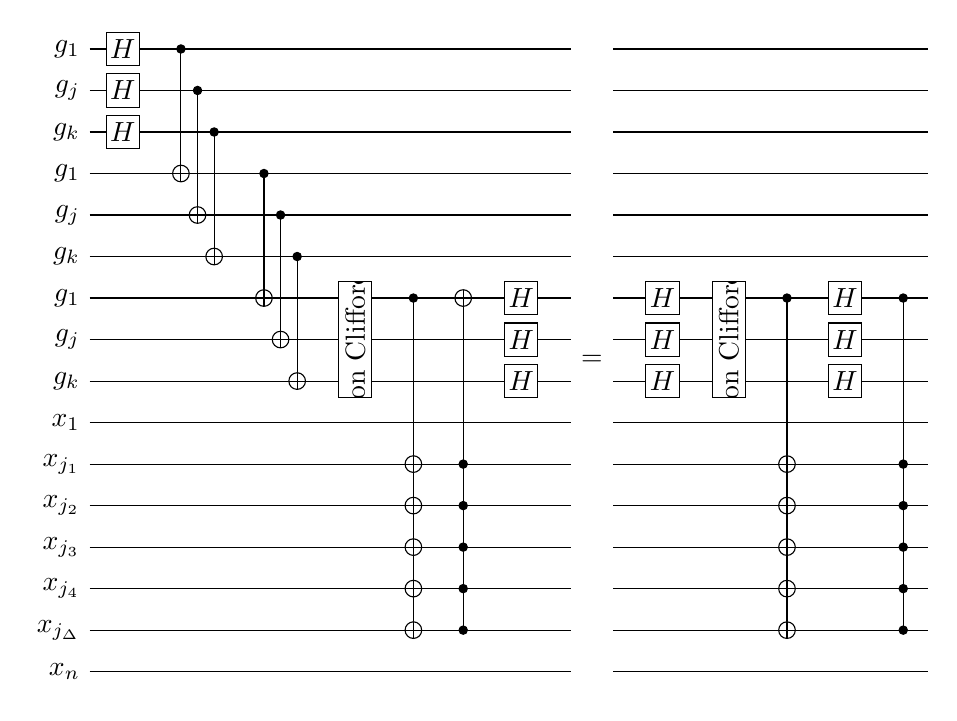
\begin{tikzpicture}[scale=1.000000,x=1pt,y=1pt]
\filldraw[color=white] (0.000000, -7.500000) rectangle (303.000000, 232.500000);
% Drawing wires
% Line 1: aa W g_1
\draw[color=black] (0.000000,225.000000) -- (303.000000,225.000000);
\draw[color=black] (0.000000,225.000000) node[left] {$g_1$};
% Line 2: cc W g_j
\draw[color=black] (0.000000,210.000000) -- (303.000000,210.000000);
\draw[color=black] (0.000000,210.000000) node[left] {$g_j$};
% Line 3: ee W g_k
\draw[color=black] (0.000000,195.000000) -- (303.000000,195.000000);
\draw[color=black] (0.000000,195.000000) node[left] {$g_k$};
% Line 4: aaa W g_1
\draw[color=black] (0.000000,180.000000) -- (303.000000,180.000000);
\draw[color=black] (0.000000,180.000000) node[left] {$g_1$};
% Line 5: ccc W g_j
\draw[color=black] (0.000000,165.000000) -- (303.000000,165.000000);
\draw[color=black] (0.000000,165.000000) node[left] {$g_j$};
% Line 6: eee W g_k
\draw[color=black] (0.000000,150.000000) -- (303.000000,150.000000);
\draw[color=black] (0.000000,150.000000) node[left] {$g_k$};
% Line 7: a W g_1
\draw[color=black] (0.000000,135.000000) -- (303.000000,135.000000);
\draw[color=black] (0.000000,135.000000) node[left] {$g_1$};
% Line 8: c W g_j
\draw[color=black] (0.000000,120.000000) -- (303.000000,120.000000);
\draw[color=black] (0.000000,120.000000) node[left] {$g_j$};
% Line 9: e W g_k
\draw[color=black] (0.000000,105.000000) -- (303.000000,105.000000);
\draw[color=black] (0.000000,105.000000) node[left] {$g_k$};
% Line 11: a2 W x_1
\draw[color=black] (0.000000,90.000000) -- (303.000000,90.000000);
\draw[color=black] (0.000000,90.000000) node[left] {$x_1$};
% Line 12: c2 W x_{j_1}
\draw[color=black] (0.000000,75.000000) -- (303.000000,75.000000);
\draw[color=black] (0.000000,75.000000) node[left] {$x_{j_1}$};
% Line 13: c21 W x_{j_2}
\draw[color=black] (0.000000,60.000000) -- (303.000000,60.000000);
\draw[color=black] (0.000000,60.000000) node[left] {$x_{j_2}$};
% Line 14: c22 W x_{j_3}
\draw[color=black] (0.000000,45.000000) -- (303.000000,45.000000);
\draw[color=black] (0.000000,45.000000) node[left] {$x_{j_3}$};
% Line 15: c23 W x_{j_4}
\draw[color=black] (0.000000,30.000000) -- (303.000000,30.000000);
\draw[color=black] (0.000000,30.000000) node[left] {$x_{j_4}$};
% Line 16: c24 W x_{j_\Delta}
\draw[color=black] (0.000000,15.000000) -- (303.000000,15.000000);
\draw[color=black] (0.000000,15.000000) node[left] {$x_{j_\Delta}$};
% Line 17: e2 W x_n
\draw[color=black] (0.000000,0.000000) -- (303.000000,0.000000);
\draw[color=black] (0.000000,0.000000) node[left] {$x_n$};
% Done with wires; drawing gates
% Line 19: aa H
\begin{scope}
\draw[fill=white] (12.000000, 225.000000) +(-45.000000:8.485281pt and 8.485281pt) -- +(45.000000:8.485281pt and 8.485281pt) -- +(135.000000:8.485281pt and 8.485281pt) -- +(225.000000:8.485281pt and 8.485281pt) -- cycle;
\clip (12.000000, 225.000000) +(-45.000000:8.485281pt and 8.485281pt) -- +(45.000000:8.485281pt and 8.485281pt) -- +(135.000000:8.485281pt and 8.485281pt) -- +(225.000000:8.485281pt and 8.485281pt) -- cycle;
\draw (12.000000, 225.000000) node {$H$};
\end{scope}
% Line 20: cc H
\begin{scope}
\draw[fill=white] (12.000000, 210.000000) +(-45.000000:8.485281pt and 8.485281pt) -- +(45.000000:8.485281pt and 8.485281pt) -- +(135.000000:8.485281pt and 8.485281pt) -- +(225.000000:8.485281pt and 8.485281pt) -- cycle;
\clip (12.000000, 210.000000) +(-45.000000:8.485281pt and 8.485281pt) -- +(45.000000:8.485281pt and 8.485281pt) -- +(135.000000:8.485281pt and 8.485281pt) -- +(225.000000:8.485281pt and 8.485281pt) -- cycle;
\draw (12.000000, 210.000000) node {$H$};
\end{scope}
% Line 21: ee H
\begin{scope}
\draw[fill=white] (12.000000, 195.000000) +(-45.000000:8.485281pt and 8.485281pt) -- +(45.000000:8.485281pt and 8.485281pt) -- +(135.000000:8.485281pt and 8.485281pt) -- +(225.000000:8.485281pt and 8.485281pt) -- cycle;
\clip (12.000000, 195.000000) +(-45.000000:8.485281pt and 8.485281pt) -- +(45.000000:8.485281pt and 8.485281pt) -- +(135.000000:8.485281pt and 8.485281pt) -- +(225.000000:8.485281pt and 8.485281pt) -- cycle;
\draw (12.000000, 195.000000) node {$H$};
\end{scope}
% Line 23: aa +aaa
\draw (33.000000,225.000000) -- (33.000000,180.000000);
\filldraw (33.000000, 225.000000) circle(1.500000pt);
\begin{scope}
\draw[fill=white] (33.000000, 180.000000) circle(3.000000pt);
\clip (33.000000, 180.000000) circle(3.000000pt);
\draw (30.000000, 180.000000) -- (36.000000, 180.000000);
\draw (33.000000, 177.000000) -- (33.000000, 183.000000);
\end{scope}
% Line 24: cc +ccc
\draw (39.000000,210.000000) -- (39.000000,165.000000);
\filldraw (39.000000, 210.000000) circle(1.500000pt);
\begin{scope}
\draw[fill=white] (39.000000, 165.000000) circle(3.000000pt);
\clip (39.000000, 165.000000) circle(3.000000pt);
\draw (36.000000, 165.000000) -- (42.000000, 165.000000);
\draw (39.000000, 162.000000) -- (39.000000, 168.000000);
\end{scope}
% Line 25: ee +eee
\draw (45.000000,195.000000) -- (45.000000,150.000000);
\filldraw (45.000000, 195.000000) circle(1.500000pt);
\begin{scope}
\draw[fill=white] (45.000000, 150.000000) circle(3.000000pt);
\clip (45.000000, 150.000000) circle(3.000000pt);
\draw (42.000000, 150.000000) -- (48.000000, 150.000000);
\draw (45.000000, 147.000000) -- (45.000000, 153.000000);
\end{scope}
% Line 27: aaa +a
\draw (63.000000,180.000000) -- (63.000000,135.000000);
\filldraw (63.000000, 180.000000) circle(1.500000pt);
\begin{scope}
\draw[fill=white] (63.000000, 135.000000) circle(3.000000pt);
\clip (63.000000, 135.000000) circle(3.000000pt);
\draw (60.000000, 135.000000) -- (66.000000, 135.000000);
\draw (63.000000, 132.000000) -- (63.000000, 138.000000);
\end{scope}
% Line 28: ccc +c
\draw (69.000000,165.000000) -- (69.000000,120.000000);
\filldraw (69.000000, 165.000000) circle(1.500000pt);
\begin{scope}
\draw[fill=white] (69.000000, 120.000000) circle(3.000000pt);
\clip (69.000000, 120.000000) circle(3.000000pt);
\draw (66.000000, 120.000000) -- (72.000000, 120.000000);
\draw (69.000000, 117.000000) -- (69.000000, 123.000000);
\end{scope}
% Line 29: eee +e
\draw (75.000000,150.000000) -- (75.000000,105.000000);
\filldraw (75.000000, 150.000000) circle(1.500000pt);
\begin{scope}
\draw[fill=white] (75.000000, 105.000000) circle(3.000000pt);
\clip (75.000000, 105.000000) circle(3.000000pt);
\draw (72.000000, 105.000000) -- (78.000000, 105.000000);
\draw (75.000000, 102.000000) -- (75.000000, 108.000000);
\end{scope}
% Line 31: a c e G \rotatebox{90}{Non Cliffords}
\draw (96.000000,135.000000) -- (96.000000,105.000000);
\begin{scope}
\draw[fill=white] (96.000000, 120.000000) +(-45.000000:8.485281pt and 29.698485pt) -- +(45.000000:8.485281pt and 29.698485pt) -- +(135.000000:8.485281pt and 29.698485pt) -- +(225.000000:8.485281pt and 29.698485pt) -- cycle;
\clip (96.000000, 120.000000) +(-45.000000:8.485281pt and 29.698485pt) -- +(45.000000:8.485281pt and 29.698485pt) -- +(135.000000:8.485281pt and 29.698485pt) -- +(225.000000:8.485281pt and 29.698485pt) -- cycle;
\draw (96.000000, 120.000000) node {\rotatebox{90}{Non Cliffords}};
\end{scope}
% Line 33: a +c2 +c21 +c22 +c23 +c24
\draw (117.000000,135.000000) -- (117.000000,15.000000);
\filldraw (117.000000, 135.000000) circle(1.500000pt);
\begin{scope}
\draw[fill=white] (117.000000, 75.000000) circle(3.000000pt);
\clip (117.000000, 75.000000) circle(3.000000pt);
\draw (114.000000, 75.000000) -- (120.000000, 75.000000);
\draw (117.000000, 72.000000) -- (117.000000, 78.000000);
\end{scope}
\begin{scope}
\draw[fill=white] (117.000000, 60.000000) circle(3.000000pt);
\clip (117.000000, 60.000000) circle(3.000000pt);
\draw (114.000000, 60.000000) -- (120.000000, 60.000000);
\draw (117.000000, 57.000000) -- (117.000000, 63.000000);
\end{scope}
\begin{scope}
\draw[fill=white] (117.000000, 45.000000) circle(3.000000pt);
\clip (117.000000, 45.000000) circle(3.000000pt);
\draw (114.000000, 45.000000) -- (120.000000, 45.000000);
\draw (117.000000, 42.000000) -- (117.000000, 48.000000);
\end{scope}
\begin{scope}
\draw[fill=white] (117.000000, 30.000000) circle(3.000000pt);
\clip (117.000000, 30.000000) circle(3.000000pt);
\draw (114.000000, 30.000000) -- (120.000000, 30.000000);
\draw (117.000000, 27.000000) -- (117.000000, 33.000000);
\end{scope}
\begin{scope}
\draw[fill=white] (117.000000, 15.000000) circle(3.000000pt);
\clip (117.000000, 15.000000) circle(3.000000pt);
\draw (114.000000, 15.000000) -- (120.000000, 15.000000);
\draw (117.000000, 12.000000) -- (117.000000, 18.000000);
\end{scope}
% Line 34: +a c2 c21 c22 c23 c24
\draw (135.000000,135.000000) -- (135.000000,15.000000);
\begin{scope}
\draw[fill=white] (135.000000, 135.000000) circle(3.000000pt);
\clip (135.000000, 135.000000) circle(3.000000pt);
\draw (132.000000, 135.000000) -- (138.000000, 135.000000);
\draw (135.000000, 132.000000) -- (135.000000, 138.000000);
\end{scope}
\filldraw (135.000000, 75.000000) circle(1.500000pt);
\filldraw (135.000000, 60.000000) circle(1.500000pt);
\filldraw (135.000000, 45.000000) circle(1.500000pt);
\filldraw (135.000000, 30.000000) circle(1.500000pt);
\filldraw (135.000000, 15.000000) circle(1.500000pt);
% Line 36: a H
\begin{scope}
\draw[fill=white] (156.000000, 135.000000) +(-45.000000:8.485281pt and 8.485281pt) -- +(45.000000:8.485281pt and 8.485281pt) -- +(135.000000:8.485281pt and 8.485281pt) -- +(225.000000:8.485281pt and 8.485281pt) -- cycle;
\clip (156.000000, 135.000000) +(-45.000000:8.485281pt and 8.485281pt) -- +(45.000000:8.485281pt and 8.485281pt) -- +(135.000000:8.485281pt and 8.485281pt) -- +(225.000000:8.485281pt and 8.485281pt) -- cycle;
\draw (156.000000, 135.000000) node {$H$};
\end{scope}
% Line 37: c H
\begin{scope}
\draw[fill=white] (156.000000, 120.000000) +(-45.000000:8.485281pt and 8.485281pt) -- +(45.000000:8.485281pt and 8.485281pt) -- +(135.000000:8.485281pt and 8.485281pt) -- +(225.000000:8.485281pt and 8.485281pt) -- cycle;
\clip (156.000000, 120.000000) +(-45.000000:8.485281pt and 8.485281pt) -- +(45.000000:8.485281pt and 8.485281pt) -- +(135.000000:8.485281pt and 8.485281pt) -- +(225.000000:8.485281pt and 8.485281pt) -- cycle;
\draw (156.000000, 120.000000) node {$H$};
\end{scope}
% Line 38: e H
\begin{scope}
\draw[fill=white] (156.000000, 105.000000) +(-45.000000:8.485281pt and 8.485281pt) -- +(45.000000:8.485281pt and 8.485281pt) -- +(135.000000:8.485281pt and 8.485281pt) -- +(225.000000:8.485281pt and 8.485281pt) -- cycle;
\clip (156.000000, 105.000000) +(-45.000000:8.485281pt and 8.485281pt) -- +(45.000000:8.485281pt and 8.485281pt) -- +(135.000000:8.485281pt and 8.485281pt) -- +(225.000000:8.485281pt and 8.485281pt) -- cycle;
\draw (156.000000, 105.000000) node {$H$};
\end{scope}
% Line 40: =
\draw[fill=white,color=white] (174.000000, -6.000000) rectangle (189.000000, 231.000000);
\draw (181.500000, 112.500000) node {$=$};
% Line 41: a H
\begin{scope}
\draw[fill=white] (207.000000, 135.000000) +(-45.000000:8.485281pt and 8.485281pt) -- +(45.000000:8.485281pt and 8.485281pt) -- +(135.000000:8.485281pt and 8.485281pt) -- +(225.000000:8.485281pt and 8.485281pt) -- cycle;
\clip (207.000000, 135.000000) +(-45.000000:8.485281pt and 8.485281pt) -- +(45.000000:8.485281pt and 8.485281pt) -- +(135.000000:8.485281pt and 8.485281pt) -- +(225.000000:8.485281pt and 8.485281pt) -- cycle;
\draw (207.000000, 135.000000) node {$H$};
\end{scope}
% Line 42: c H
\begin{scope}
\draw[fill=white] (207.000000, 120.000000) +(-45.000000:8.485281pt and 8.485281pt) -- +(45.000000:8.485281pt and 8.485281pt) -- +(135.000000:8.485281pt and 8.485281pt) -- +(225.000000:8.485281pt and 8.485281pt) -- cycle;
\clip (207.000000, 120.000000) +(-45.000000:8.485281pt and 8.485281pt) -- +(45.000000:8.485281pt and 8.485281pt) -- +(135.000000:8.485281pt and 8.485281pt) -- +(225.000000:8.485281pt and 8.485281pt) -- cycle;
\draw (207.000000, 120.000000) node {$H$};
\end{scope}
% Line 43: e H
\begin{scope}
\draw[fill=white] (207.000000, 105.000000) +(-45.000000:8.485281pt and 8.485281pt) -- +(45.000000:8.485281pt and 8.485281pt) -- +(135.000000:8.485281pt and 8.485281pt) -- +(225.000000:8.485281pt and 8.485281pt) -- cycle;
\clip (207.000000, 105.000000) +(-45.000000:8.485281pt and 8.485281pt) -- +(45.000000:8.485281pt and 8.485281pt) -- +(135.000000:8.485281pt and 8.485281pt) -- +(225.000000:8.485281pt and 8.485281pt) -- cycle;
\draw (207.000000, 105.000000) node {$H$};
\end{scope}
% Line 44: a c e G \rotatebox{90}{Non Cliffords}
\draw (231.000000,135.000000) -- (231.000000,105.000000);
\begin{scope}
\draw[fill=white] (231.000000, 120.000000) +(-45.000000:8.485281pt and 29.698485pt) -- +(45.000000:8.485281pt and 29.698485pt) -- +(135.000000:8.485281pt and 29.698485pt) -- +(225.000000:8.485281pt and 29.698485pt) -- cycle;
\clip (231.000000, 120.000000) +(-45.000000:8.485281pt and 29.698485pt) -- +(45.000000:8.485281pt and 29.698485pt) -- +(135.000000:8.485281pt and 29.698485pt) -- +(225.000000:8.485281pt and 29.698485pt) -- cycle;
\draw (231.000000, 120.000000) node {\rotatebox{90}{Non Cliffords}};
\end{scope}
% Line 45: a +c2 +c21 +c22 +c23 +c24
\draw (252.000000,135.000000) -- (252.000000,15.000000);
\filldraw (252.000000, 135.000000) circle(1.500000pt);
\begin{scope}
\draw[fill=white] (252.000000, 75.000000) circle(3.000000pt);
\clip (252.000000, 75.000000) circle(3.000000pt);
\draw (249.000000, 75.000000) -- (255.000000, 75.000000);
\draw (252.000000, 72.000000) -- (252.000000, 78.000000);
\end{scope}
\begin{scope}
\draw[fill=white] (252.000000, 60.000000) circle(3.000000pt);
\clip (252.000000, 60.000000) circle(3.000000pt);
\draw (249.000000, 60.000000) -- (255.000000, 60.000000);
\draw (252.000000, 57.000000) -- (252.000000, 63.000000);
\end{scope}
\begin{scope}
\draw[fill=white] (252.000000, 45.000000) circle(3.000000pt);
\clip (252.000000, 45.000000) circle(3.000000pt);
\draw (249.000000, 45.000000) -- (255.000000, 45.000000);
\draw (252.000000, 42.000000) -- (252.000000, 48.000000);
\end{scope}
\begin{scope}
\draw[fill=white] (252.000000, 30.000000) circle(3.000000pt);
\clip (252.000000, 30.000000) circle(3.000000pt);
\draw (249.000000, 30.000000) -- (255.000000, 30.000000);
\draw (252.000000, 27.000000) -- (252.000000, 33.000000);
\end{scope}
\begin{scope}
\draw[fill=white] (252.000000, 15.000000) circle(3.000000pt);
\clip (252.000000, 15.000000) circle(3.000000pt);
\draw (249.000000, 15.000000) -- (255.000000, 15.000000);
\draw (252.000000, 12.000000) -- (252.000000, 18.000000);
\end{scope}
% Line 47: a H
\begin{scope}
\draw[fill=white] (273.000000, 135.000000) +(-45.000000:8.485281pt and 8.485281pt) -- +(45.000000:8.485281pt and 8.485281pt) -- +(135.000000:8.485281pt and 8.485281pt) -- +(225.000000:8.485281pt and 8.485281pt) -- cycle;
\clip (273.000000, 135.000000) +(-45.000000:8.485281pt and 8.485281pt) -- +(45.000000:8.485281pt and 8.485281pt) -- +(135.000000:8.485281pt and 8.485281pt) -- +(225.000000:8.485281pt and 8.485281pt) -- cycle;
\draw (273.000000, 135.000000) node {$H$};
\end{scope}
% Line 48: c H
\begin{scope}
\draw[fill=white] (273.000000, 120.000000) +(-45.000000:8.485281pt and 8.485281pt) -- +(45.000000:8.485281pt and 8.485281pt) -- +(135.000000:8.485281pt and 8.485281pt) -- +(225.000000:8.485281pt and 8.485281pt) -- cycle;
\clip (273.000000, 120.000000) +(-45.000000:8.485281pt and 8.485281pt) -- +(45.000000:8.485281pt and 8.485281pt) -- +(135.000000:8.485281pt and 8.485281pt) -- +(225.000000:8.485281pt and 8.485281pt) -- cycle;
\draw (273.000000, 120.000000) node {$H$};
\end{scope}
% Line 49: e H
\begin{scope}
\draw[fill=white] (273.000000, 105.000000) +(-45.000000:8.485281pt and 8.485281pt) -- +(45.000000:8.485281pt and 8.485281pt) -- +(135.000000:8.485281pt and 8.485281pt) -- +(225.000000:8.485281pt and 8.485281pt) -- cycle;
\clip (273.000000, 105.000000) +(-45.000000:8.485281pt and 8.485281pt) -- +(45.000000:8.485281pt and 8.485281pt) -- +(135.000000:8.485281pt and 8.485281pt) -- +(225.000000:8.485281pt and 8.485281pt) -- cycle;
\draw (273.000000, 105.000000) node {$H$};
\end{scope}
% Line 51: a c2 c21 c22 c23 c24
\draw (294.000000,135.000000) -- (294.000000,15.000000);
\filldraw (294.000000, 135.000000) circle(1.500000pt);
\filldraw (294.000000, 75.000000) circle(1.500000pt);
\filldraw (294.000000, 60.000000) circle(1.500000pt);
\filldraw (294.000000, 45.000000) circle(1.500000pt);
\filldraw (294.000000, 30.000000) circle(1.500000pt);
\filldraw (294.000000, 15.000000) circle(1.500000pt);
% Done with gates; drawing ending labels
% Done with ending labels; drawing cut lines and comments
% Done with comments
\end{tikzpicture}

\begin{figure}[h]
  \begin{subfigure}[b]{0.45\textwidth}
    \begin{claim}
      The state:
      \begin{equation*}
        \begin{split}
          \sum_{z \in C_{Z}^{\perp}}  \exp \Big(  & -  2 \cdot \pi/4 \sum_{g ,h
            \in \text{ gen } C_{Z}^{\perp}} \hat{X}_{g}\hat{X}_{h}|g\cdot h| \\
            & +  4 \cdot i\pi/4 \sum_{g,h \in \text{ gen } C_{Z}^{\perp}}
          \hat{X}_{g}\hat{X}_{h}\hat{X}_{l}|g\cdot h \cdot l|  \Big) \ket{z}
        \end{split}
      \end{equation*}
      Can be computed such that any
    \end{claim}
  \end{subfigure}
  \begin{subfigure}[b]{0.05\textwidth}
    \
  \end{subfigure}
  \begin{subfigure}[b]{0.45\textwidth}
  \end{subfigure}
\end{figure}

\begin{proof}
  Denote by $U_{v}$ the gate which turn on all the generators supported on $v$.
  As any of them is just of a code word of $C_{A}\otimes C_{B}$, namely turning
  on generator require touching at most constant number of qubits combing
\end{proof}

\begin{claim}
  \label{claim:lowlightcone}
  The state $\left(M_{2}^{\dagger}\otimes I\right)\ket{ C_{Z}^{\perp} +
  \Lambda   }\ket{0}$ can be computed, such that the light cone depth of any
  non-clifford gate is bounded by constant.
\end{claim}
\begin{proof}
  \begin{align*}
    \left( I \otimes H_{X} \right) CX_{n\rightarrow n} \left(E \otimes E
    \right) \ \ I \otimes L[M_{2}^{\dagger}] \ \ & \prod_{\substack{ J\in \{
    \text{ gen }\Lambda,\\ \text{ gen } C_{Z}^{\perp} \}}} \prod_{g \in J}
    \left(
    I +  X_{L[g]} \right) && \ket{0} \ket{0} \\
    = \left( I \otimes H_{X}   \right) CX_{n\rightarrow n} & \sum_{\substack{ z
    \in C_{Z}^\perp \\  x\in \Lambda}}  e^{\varphi(z)} && \ket{x}\ket{z} \\
    = & \sum_{\substack{ z \in C_{Z}^\perp \\  x\in \Lambda}}   e^{\varphi(z)}
    && \ket{x+z}\ket{0} \\
    = & \sum_{\substack{ z \in C_{Z}^\perp \\  x\in \Lambda}}
    \left(M_{2}^{\dagger}\otimes I\right) && \ket{x+z}\ket{0} \\
    = & \left(M_{2}^{\dagger}\otimes I\right) && \ket{ C_{Z}^{\perp} +
    \Lambda   }\ket{0}
  \end{align*}
\end{proof}
Denote by $p \in [0,1]$ the error rate of input magic states, and let $\ket{A}$
be an ancilla initialized to a one-qubit magic state. This $\ket{A}$ can be
used to compute the $T$ gate, with a probability of $Z$ error occurring with a
probability of $p$ \cite{bravyi2012magic}.
\begin{claim}
  There are constant numbers $\zeta_{\Delta},\xi_{\Delta}$, and a circuit
  $\mathcal{C}$ such that:
  \begin{enumerate}
    \item In the no-noise setting, The circuit compute the state
      \begin{equation*}
        \begin{split}
          \mathcal{C} \ket{0}^{\Theta(n)} \otimes \ket{A}^{\Theta(n)}
          \rightarrow  \prod_{g \in \text{ gen }\Lambda} T_{g} \ket{
            C_{Z}^{\perp} +
          \Lambda   }
        \end{split}
      \end{equation*}
    \item Otherwise, the circuit computes the state
      \begin{equation*}
        \begin{split}
          \mathcal{C} \ket{0}^{\Theta(n)} \otimes \ket{A}^{\Theta(n)}
          \rightarrow Z^{e} \ \ \ \prod_{g \in \text{ gen } \Lambda} T_{g} \ket{
          C_{Z}^{\perp} +  \Lambda   }
        \end{split}
      \end{equation*}
      , where the probability that $e_{i} = 1$ is less than $\zeta_{\Delta}
      \cdot  p$. Additionally, for any $i$, there are at most $\xi_{\Delta}$
      indices
      $j$ such that $e_{i}$ and $e_{j}$ are dependent.
  \end{enumerate}
\end{claim}

\begin{proof}
  Concatinate the $T^{n} \otimes I $ with the gate in \Cref{claim:lowlightcone}.
\end{proof}

\begin{claim}
  For any $\alpha \in (0,1)$ the probability that
  $|e|>(1+\alpha)p\zeta_{\Delta}$ is less than:
  \begin{equation*}
    \begin{split}
      \prb{ |e| > (1+\alpha) \expp{|e|} } < \frac{1\cdot
      \xi_{\Delta}n}{\alpha^{2}\zeta_{\Delta}^{2}p^{2}n^{2}} = o\left( 1/n
      \right)
    \end{split}
  \end{equation*}
\end{claim}
\begin{proof}
  By the Chebyshev inequality, notice that the number for which
  $\expp{e_{i}e_{j}}-\expp{e_{i}}\expp{e_{j}} \neq 0$ is less than
  $\xi_{\Delta}n$.
\end{proof}

\begin{definition}
  We will said that a decoder $\mathcal{D}$ for the good qunatum LDPC code is
  an good-local decoder if
  \begin{enumerate}
    \item There is a treashold $\mu n$ such that if the error size is less than
      $|e| < \mu n$ then $\mathcal{D}$ correct $e$ in constant number of rounds.
      With probability $ 1 - o(1/n)$.
    \item In any rounds $\mathcal{D}$ performs at most $O(n)$ work (depth
      $\times$ width).
    \item The above is true in operation-noisy settings, where there is a
      probability of $p$ for an error to occur after acting on a qubit.
      ($\star$)
  \end{enumerate}
  $\star$ The motivation for this is that if the decoder does not act on the
  qubit, then it also does not apply a $T$ gate on it. Therefore, in the
  distillation setting, there is zero chance for an error to occur.
\end{definition}

\begin{claim}
  Suppose there is a good local decoder $\mathcal{D}$ for the good qLDPC code.
  Then, there exists $p_{0}$ such that for any sufficiently large $n$, there is
  a distillation protocol that, given $\Theta(n)$ magic states at an error rate
  $p<p_{0}$, successfully distills $\Theta(n)$ perfect magic states with a
  probability of $1 - o(1/n)$. Furthermore, the protocol's space and time
  complexity (both quantum and classical) are $\Theta(n)$ and $\Theta(n^{2})$,
  respectively.
\end{claim}

\ifdefined\MORE

\begin{figure}[h]
  \begin{subfigure}[t]{0.65\textwidth}
    \begin{definition}
      Let $M \in \mathbb{F}_{2}^{k \times n }$ upper triangular matrix such
      that~$k~<~n$. We say that $M$ has the $1$-stairs property if $M_{ij}=1$
      any
      $j<i$.
    \end{definition}
    \begin{claim}
      \label{claim:stair}
      Any $M \in \mathbb{F}_{2}^{k \times n }$ upper triangular matrix can be
      turn into upper triangular matrix that has the $1$-stairs property by
      elementary operation.
    \end{claim}

  \end{subfigure}
  \begin{subfigure}[t]{0.05\textwidth}
    \
  \end{subfigure}
  \begin{subfigure}[t]{0.25\textwidth}

    \begin{equation*}
      \begin{split}
        \begin{bmatrix}
          1 & 1 & 1 &1 &1 &\cdot & \cdot & \cdot & \cdot & \cdot \\
          0 & 1 & 1 &1 &1 &\cdot & \cdot & \cdot & \cdot & \cdot \\
          0 & 0 & 1 &1 &1 &\cdot & \cdot & \cdot & \cdot & \cdot \\
          0 & 0 & 0 &1 &1 &\cdot & \cdot & \cdot & \cdot & \cdot \\
          0 & 0 & 0 &0 &1 &\cdot & \cdot & \cdot & \cdot & \cdot
        \end{bmatrix}
      \end{split}
    \end{equation*}

  \end{subfigure}
\end{figure}
\begin{proof}
  Consider the following algorithm: Let $M$ be our initial matrix. We iterate
  over the rows from left to right. In the $i$th iteration, we check for any row
  $j<i$ if $M_{ji} = 1$. If not, we set $M$ to be the matrix obtained by adding
  the $i$th row to the $j$th row. Since $M$ is an upper triangular matrix,
  adding the $i$th row does not change any entry $M_{js}$ for $s<i$. Therefore,
  the obtained matrix is still an upper triangular matrix and the entries at
  $M_{js}$ for $j,s < i$ remain the same, namely $1$ if and only if $j\le s$.

  Continuing with the process eventually yields, after $k$ iterations, a matrix
  with the $1$-stair property.
\end{proof}

\begin{claim}
  The logical operator $CX_{g}$ relative the code $C_{Z}^{\perp}$ can be
  implement such it acts on constant number of qubits. \textbf{Notice,}
  implementation of the gate $CX_{g}$ relative to $C_{Z}^{\perp}$ might
  incorrect for computing $CX_{g}$ relative to $C_{X}$.
\end{claim}

\begin{definition}[Source of $g \in C_{Z}^{\perp}$.]
  Let $C$ be the quantum Tanner code, and let $g$ be a generator of
  $C_{Z}^{\perp}$. The vertex $v$ will be called the source of $g$. If $g$ is a
  codeword of the tensor code $C_{A}\otimes C_{B}$, it can be viewed locally on
  $g$.
\end{definition}

\begin{figure}[h]
  \begin{subfigure}{0.5\textwidth}
    \begin{proof}
      Let $g$ be a generator of $C_{Z}^{\perp}$. As the generators of
      $C_{Z}^\perp$ are defined to be the set of codewords of some 'small code'
      ($C_{0}$) over the local view of the vertices in a $\Delta$-regular
      graph, it
      holds that first, there is a vertex $v$ on which $g$ is supported. Second,
      only the generators supported by $v$'s neighbors have a non-vanishing
      overlap
      with $g$.

      Let $g$ be a generator of $C_{Z}^{\perp}$ and denote by $v$ the source of
      $g$. First, we will prove that there exist $\xi_{1}, \xi_{2}, \xi_{3} \in
      \mathbb{F}_{2}^{N}$ such that each $\xi_{i}$ has a weight of at most
      $\frac{1}{2} \Delta$, $\xi_{i} \cdot g = 1$, and for any other generator
      $h
      \neq g$ in $C_{Z}^{\perp}$, there is at least one $i$ such that $\xi_{i}
      \cdot
      h = 0$.

      Let $B_1, B_2, B_3$ be subsets of $[\Delta]$ such that $|B_i| =
      \frac{2}{3}\Delta$ and $B_1 \cap B_2 \cap B_3 = \emptyset$. Now, define
      $\xi_i$ to be the vector supported only on $B_i$ and satisfies $\xi_i
      \cdot g
      = 1$. For any other generator $h$ such that $v$ is its source, and also
      $h|_{B_{i}} \neq g|_{B_{i}}$, we have $\xi_i \cdot h = 0$. Notice that for
      every $h \neq g$, there must be at least one $B_{i}$ for which $g|_{B_{i}}
      \neq h|_{B_{i}}$. Each $x_{i}$ is a solution for a linear system with (at
      most) $\rho\Delta$ equations and $\frac{1}{2} \Delta$ bits. So, if $1/2 >
      \rho$, then there is a solution for each equations system.

      Clearly, for any generator $h$ such $v$ is it's source there are not
      $i$'s such $\xi_{i}h = 1$. It's left to show for remian generators.

    \end{proof}
  \end{subfigure}
  \begin{subfigure}{0.05\textwidth}
    \
  \end{subfigure}
  \begin{subfigure}[t]{0.4\textwidth}
    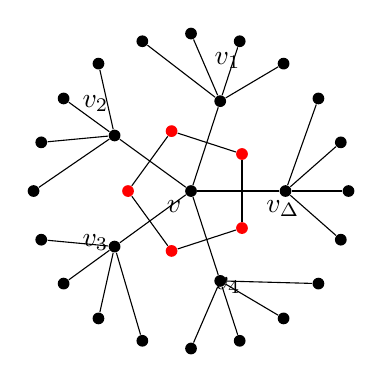
\begin{tikzpicture}
      \begin{scope}[shift={({0},{-2})}]
        \foreach \i in {1,...,5}
        \node[circle, fill=black, inner sep=1.5pt] (\i) at (72*\i:1.2) {};
        \foreach \i in {1,...,5}
        \node[circle, fill=red, inner sep=1.5pt] (\i\i) at (72*\i-36:0.8) {};

        \foreach \i in {1,...,5}
        \foreach \j in {1,...,4}
        \node[circle, fill=black, inner sep=1.5pt] (5*\i+\j) at
        (72*\i+18*\j-36:2) {};
        \node[circle, fill=black, inner sep=1.5pt] (0) at (0,0) {};
        % edges
        \foreach \i in {1,...,5}
        \draw (\i) -- (0);
        \foreach \i[evaluate=\i as \m using int(\i+1)] in {1,...,4}
        \draw (\i\i) -- (\m\m);
        \draw (55) -- (11);
        \foreach \i in {1,...,5}
        \foreach \j in {1,...,4}
        \draw (\i) -- (5*\i+\j);
        % labels
        \foreach \i in {1,...,4}
        \node[above] at (72*\i:1.5) {$v_{\i}$};
        \node[anchor=north east] at (72*5:1.5) {$v_{\Delta}$};
        \node[anchor=north east] at (0,0) {$v$};
      \end{scope}
    \end{tikzpicture}
  \end{subfigure}
\end{figure}

\begin{claim}
  Let $Q =(C_{X},C_{Z})$ a good qLDPC CSS code. Then for any $g$ generator in
  $C_{Z}^{\perp}$ there is a logical gate compute $CX_{g}$ acting on at most
  $O(1)$ qubits.
\end{claim}
\begin{proof}
  Recall that the generator matrix of $C_{Z}^\perp$ is the parity check matrix
  of $C_{Z}$. So we are looking for $\xi$ such that:
  \begin{equation*}
    \begin{split}
      H_{Z}
      \begin{bmatrix}
        | \\
        | \\
        \xi \\
        | \\
        |
      \end{bmatrix} =
      \begin{bmatrix}
        1 \\
        0 \\
        0 \\
        0 \\
        0
      \end{bmatrix}
    \end{split}
  \end{equation*}
  Assume that there is solution $\xi$ for the equations system. If $H_{z}$ is a
  parity check matrix of ltc code then $d(\xi,C_{Z}) = O(1)$ so we could picck
  some $z+\xi$ such that $z\in C_{Z}$ and having a solution that it's weight is
  $O(1)$.   %, then any $z + \xi$  where $z \in C_{Z}$ is also a solution.
  % \prod_{z_{r_i^{\prime}}}
  \begin{equation*}
    \begin{split}
      \sum_{r_{i},l_{j}}\ket{z_{r_i}}\ket{z_{l_j}} & =
      \sum_{z_{r_i^{\prime}}}\sum_{r_{i},l_{j}}\ket{z_{r_i}}\ket{z_{l_j}} \ket{
        0 +
      \xi[z_{r_{i^{\prime}}}]\cdot z_{r_{i}} } \sum_{z_{l_j^{\prime}}} \\
      x &
    \end{split}
  \end{equation*}

\end{proof}

\newcommand{\hashcode}{ checks-hashed }

\begin{definition}
  Let $\{h_{i} \}_{1}^{t}$ be the checks of $\Delta$-length code $C_{0}$. We
  say that $i$th bit and the $j$th bit collide if there a check $h$ such that
  $h_{i}=h_{j}=1$. We say that a $C_{0}$ is a \hashcode if:
  \begin{equation*}
    \begin{split}
      \prbm{ i,j \text{ collide  }  }{ i, j \sim [\Delta]^{2} } <
      \frac{1}{2\Delta}
    \end{split}
  \end{equation*}
\end{definition}

\begin{claim}
  Suppose that $C_{0}^{\perp}$ is a \hashcode. Then $\left( C_{0}^{\otimes m}
  \right)^{\perp}$ is also a \hashcode.
\end{claim}
\begin{proof}

  \begin{equation*}
    \begin{split}
      \prbm{X^{(m)}_{u,v}}{u,v\sim [n]^{2}} \le & \prbm{X^{(1)}_{u,v}}{u,v\sim
      [\Delta]^{2}} \cdot \prbm{X^{(m-1)}_{u,v} }{u,v\sim [n/\Delta]^{2}} \\
      \le & \frac{1}{2\Delta} \cdot \left( \frac{1}{2\Delta} \right)^{m-1} =
      \left( \frac{1}{2\Delta} \right)^{m}
    \end{split}
  \end{equation*}
\end{proof}

Consider the following decoder, we flip a bit if flipping it decrease the
syndrome. Now observers that if a non faulty bit $i$ has been flip then it
means that there is at least one faulty bit $j$ in the error $e$ that $i,j$
collide. Similarly if a faulty bit $i$ hasn't been flip then it means that
there is another faulty bit $j$ that collide with him. In overall we conclude
that the total number of incorrect flips made by the decoder is at most the
number of collisions.

\begin{equation*}
  \begin{split}
    \expp{\sum_{v \in e} \sum_{u \in [n]} X_{v,u}} \le |e|\cdot n \cdot \left(
    \frac{1}{2\Delta} \right)^{m} = \frac{|e|}{2^{m}}
  \end{split}
\end{equation*}

Now we are going to add a random error at weight $\frac{|e|}{2^{m}}$ to ensure
that in the next iteration the $\frac{|e|}{2^{m-1}}$ error will distributed
uniformly. Repeating for $\log_{2^{m-1}}$ rounds correct the error. (not
exactly there is an error in each round that should be handled).

\ctt{ We flip in over all $|e| \sum \frac{1}{2^{i}}  < 2|e| $ bits, so we would
like to have $|e| \le d/4 $.}

\ctt{ Yet we can do better, if $ e = z + \tilde{e}$ where $z$ commute with all
our generators. }

\ctt{ And if it anticommute with only $l$ of them, then we have only $l$
errors. }

\begin{equation*}
  \begin{split}
    \Delta^{m}\le 1/p^{2}_{0} & \rightarrow \alpha \cdot 1/p^{2}_{0} ,
    \frac{m}{2^{m}} \log \Delta
  \end{split}
\end{equation*}

\begin{claim}
  Let $H$ be a $|V|\times r$ binary parity check matrix of $\tilde{C}$. Also,
  let $G$ be a $\Delta$-regular graph. A bit assignment over $G$ edges $x$ will
  be said to be $\tilde{C}$-vertices-respect if the vector $z(x) \in
  \mathbb{F}_{2}^{|V|}$ which is defined as:
  \begin{equation*}
    z(x)_{v} =
    \begin{cases}
      1 & v \text{ sees at least one } 1\\
      0 & \text{otherwise}
    \end{cases}
  \end{equation*}
  is a codeword of $\tilde{C}$. Let $\Lambda$ be the set of all
  $\tilde{C}$-vertices-respect assignments. Then $|\Lambda| >
  (1-\varepsilon)2^{\rho |V|}$.
\end{claim}

\begin{proof}
  Any $x \in \Lambda$ is a solution for the following system of equations:
  \begin{equation*}
    \begin{split}
      z_{v} &= 1 + \prod_{ e \in v }{ \left( 1 - x_{e} \right) } \\
      Hz &= 0
    \end{split}
  \end{equation*}
\end{proof}

\begin{claim}
  Assume that $C_{0}$ is a $\Delta$-length code such that for any two
  non-trival codewords $c,c^{\prime}\in C_{0}$ we have that $c\cdot
  c^{\prime}=1$, and denote by $C = \mathcal{T}(G,C_{0})$. And let $\Lambda$ be
  a the set of all $\tilde{C}$-vertices-respect assignments where $\tilde{C}$
  satisfies relation $R$. Then also $C \cap \Lambda$ satisfies $R$.
\end{claim}

Let $\ket{f}$ be a codeword in $C_{X}$, and let $X_{g}$ be the indicator that
equals $1$ if $f$ has support on $X_{g}$, and $0$ otherwise. Observes that
applying $T^{\otimes}$ on $\ket{f}$ yilds the state:
\begin{equation*}
  \begin{split}
    T^{\otimes n}\ket{f} & =  T^{\otimes n}\ket{\sum_{g} X_{g}g } = \exp \Big(
      i\pi/4 \sum_{g} X_{g}|g|  -  2 \cdot i \pi/4 \sum_{g,h} X_{g}X_{h}|g\cdot
      h| \\
      & +  4 \cdot i\pi/4 \sum_{g,h} X_{g}X_{h}X_{l}|g\cdot h \cdot l| -   8
    \cdot i\pi/4 \cdot \text{ integers } \Big) \ket{f} \\
    & = \exp \Big( i\pi/4 \sum_{g} X_{g}|g|  -  2 \cdot \pi/4 \sum_{g,h}
      X_{g}X_{h}|g\cdot h| +  4 \cdot i\pi/4 \sum_{g,h} X_{g}X_{h}X_{l}|g\cdot h
    \cdot l| \Big) \ket{f}
  \end{split}
\end{equation*}

\section{Many to One.}
Assume that $f$ is supported on exactly one generator. Then we have that
$T^{\otimes n}\ket{f}  = e^{i\pi|g|/4}\ket{f}$ Therefore, if $|g| = 4k+1$ then
we are done.

\section{Using Quntum Error Correction Codes.}

Now assume that the code $C_{X}$ is the quantum Tanner code, denote by $G,A,B$
the group and the two generator sets that are used for constructing the square
complex.

\begin{claim}
  Consider $g,h$ that are supported on the same $v\in V$. We will call such a
  pair a source-sharing pair. Suppose that for any we have that $|g \cdot h|$ is
  even. Then there is a Clifford gate that computes $\ket{f} \mapsto \exp \Big(
  -  i\pi \sum_{g,h \text{ source-sharing }} X_{g}X_{h}|g\cdot h|  \Big) \ket{f}
  $.
\end{claim}
%
%%\begin{claim}
%%  \label{claim:phase}
%%  The gate $\ket{f} \mapsto \exp \Big(   i\pi \sum_{g,h}
% X_{g}X_{h}X_{l}|g\cdot h \cdot l| \Big) \ket{f} $ is in the Clifford group.
%%\end{claim}
%%
%%\begin{proof}
%%  Just decode $f$ and apply \textbf{CCZ} between any triple of qubits
% corresponding to the generators $g,h,l$ such that $g \cdot h \cdot l=_{2} 1$.
% Then encode the state again. Observes that \textbf{CCZ} is a Clifford gate,
% and by the fact that the code is a CSS code then the decoder and the encoder
% are both in the Clifford.
%%\end{proof}
%%
%
%
%\section{Fail Attempt.}
%
%
%In addition, let us assume the existence of $d \in G$ such that $d$ is
% non-identity and commutes with any element in $A \cup B$. Then, observe that
% multiplying by $d$ preserves adjacency on the complex. Namely, if $\{u,v\}
% \in E$ then also $\{du, dv\} \in E$.
%
%Consider $\ket{f}$ such that if $X_g$ is not zero, and $g$ is associated with
% a local codeword $c \in C_A \otimes C_B$ on vertex $v$, then the generator
% associated with the local codeword $c$ on vertex $d \cdot v$ also supports
% $f$, denoted by $g'$. Thus, the exponent above becomes:
%
%\begin{equation*}
%  \begin{split}
%    & = \exp \Big( i\pi/4 \sum_{g} X_{g}|g|  -  2 \cdot \pi/4 \sum_{g,h \in G
% /a} X_{g}X_{h}|g\cdot h| + X_{g^{\prime}}X_{h^{\prime}}|g\cdot h |  \\
%    & +  4 \cdot i\pi/4 \sum_{g,h \in G/a} X_{g}X_{h}X_{l}|g\cdot h \cdot l| +
% X_{g^{\prime}}X_{h^{\prime}}X_{l^{\prime}}|g\cdot h \cdot l| \Big) \ket{f} \\
%    & = \exp \Big( i\pi/4 \sum_{g} X_{g}|g|  -  2 \cdot 2 \cdot \pi/4
% \sum_{g,h \in G/a} X_{g}X_{h}|g\cdot h| +  2 \cdot 4 \cdot i\pi/4 \sum_{g,h
% \in G/a} X_{g}X_{h}X_{l}|g\cdot h \cdot l| \Big) \ket{f} \\
%    & = \exp \Big( i\pi/4 \sum_{g} X_{g}|g|  -  i\pi \sum_{g,h \in G/a}
% X_{g}X_{h}|g\cdot h|  \Big) \ket{f}
%  \end{split}
%\end{equation*}
%
%\begin{figure}
%  \centering
%  \scalebox{0.1}{
%    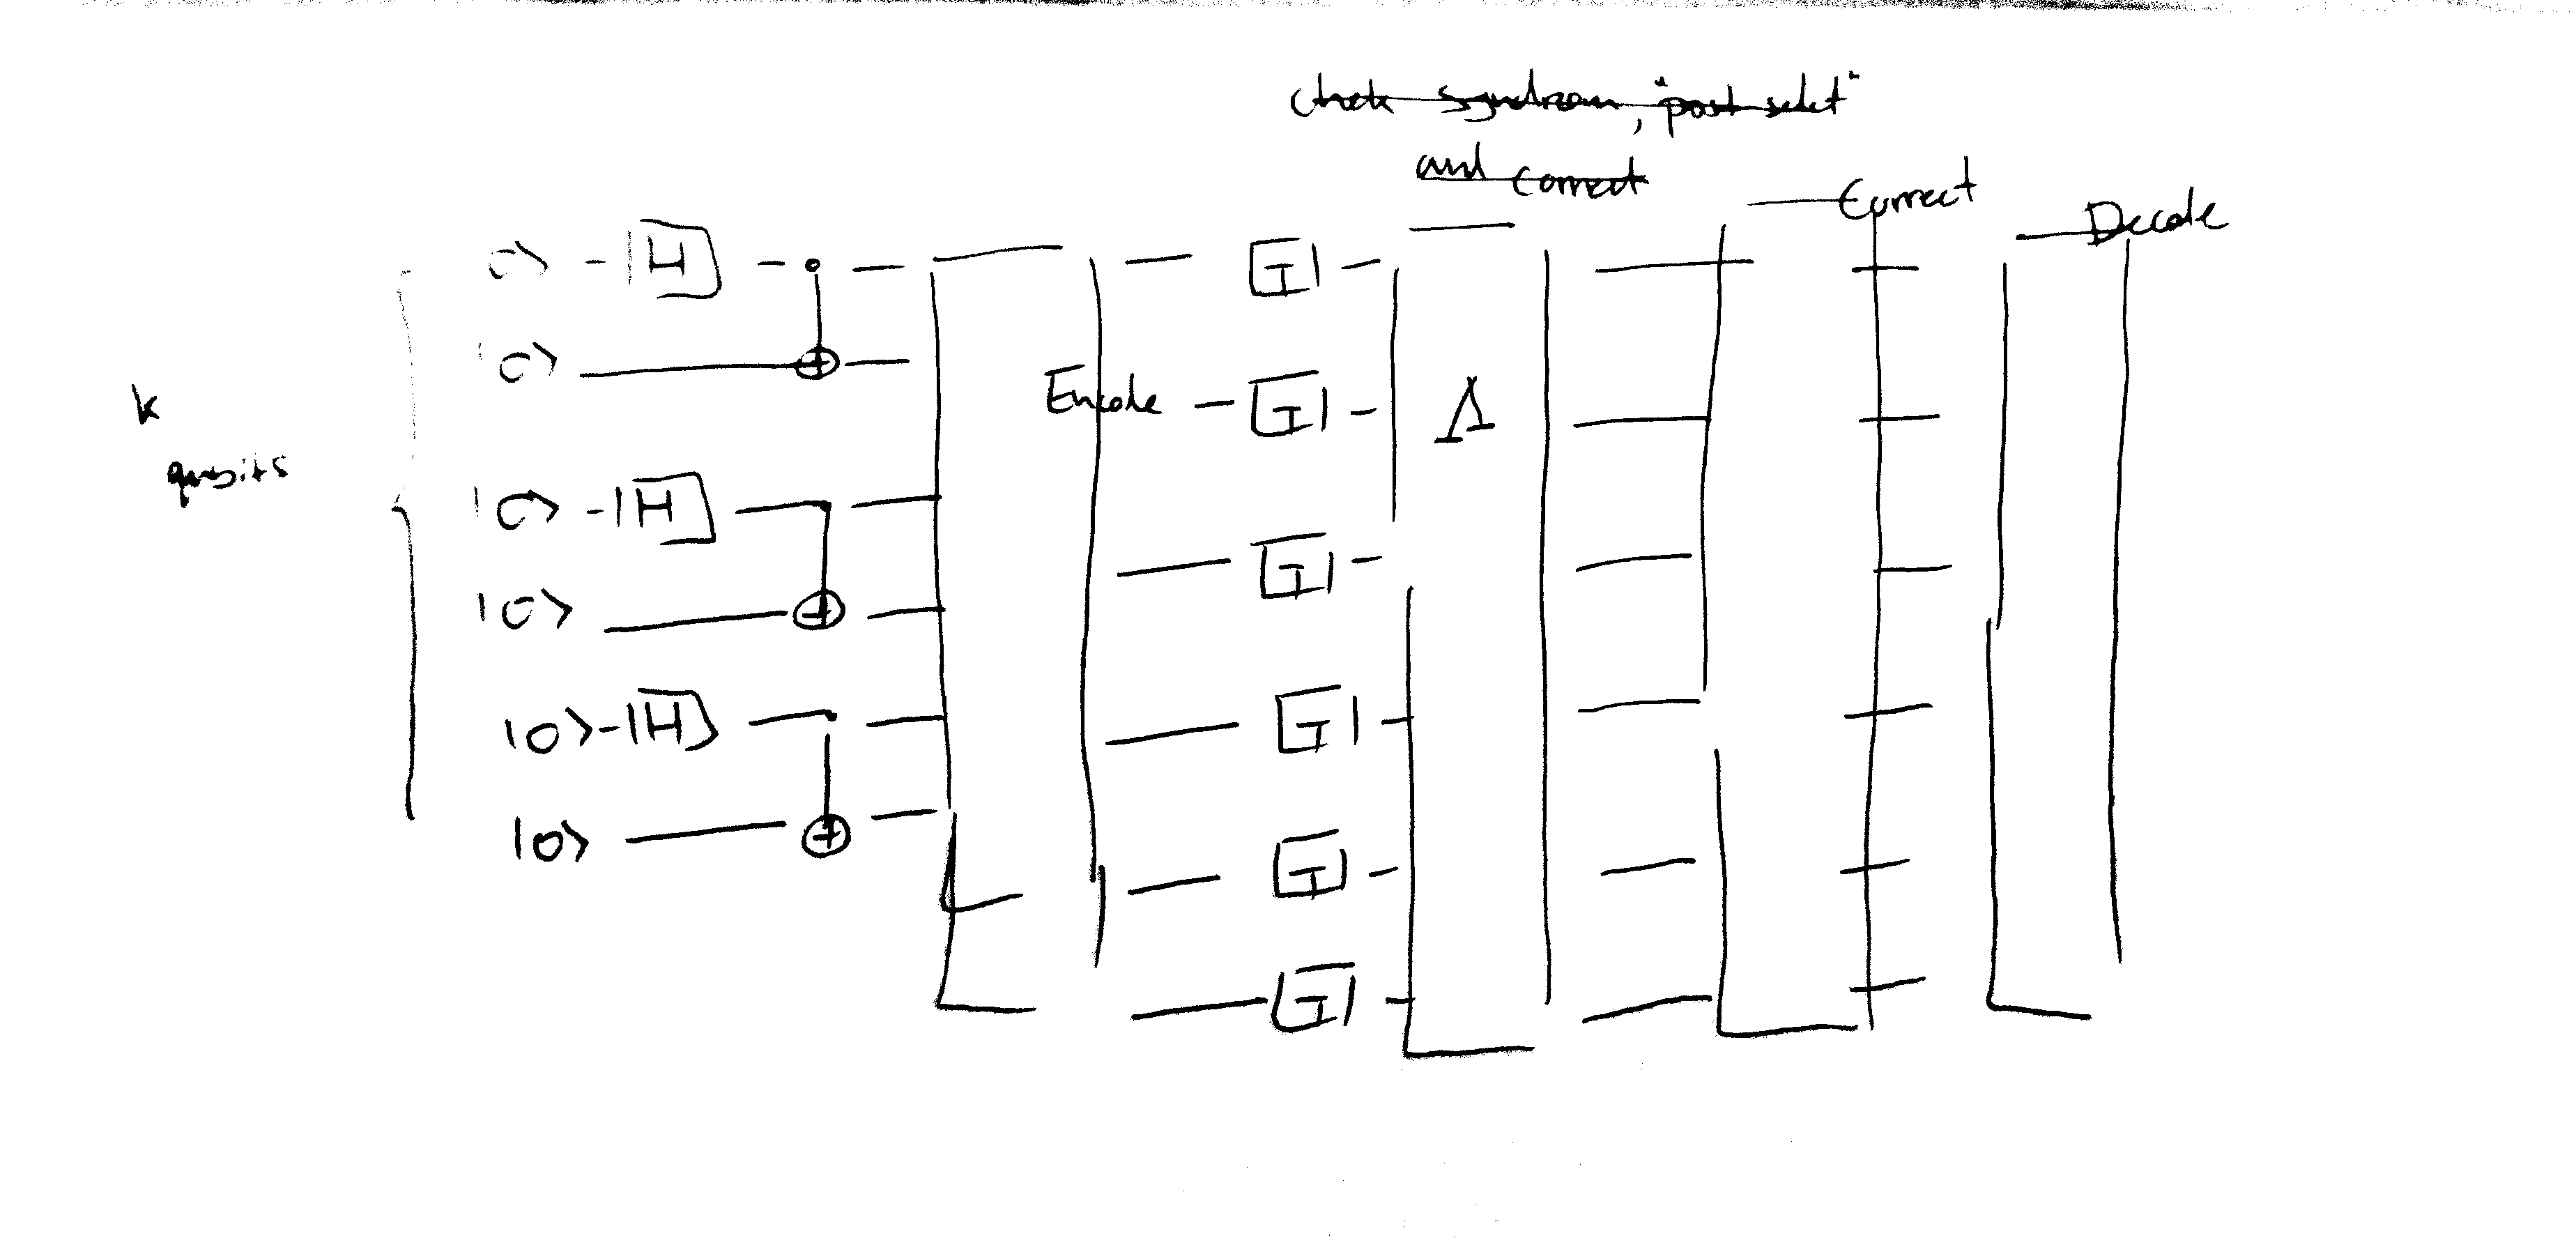
\includegraphics{distil.jpg-out.png}
%}
%  \caption{Quantum Circuit for distillation.}
%  \label{fig:circuit}
%\end{figure}
%
%\begin{claim}
%  \label{claim:phase}
%  The gate $\ket{f} \mapsto \exp \Big(  -  i\pi \sum_{g,h \in G/a}
% X_{g}X_{h}|g\cdot h|  \Big) \ket{f} $ is in the Clifford.
%\end{claim}
%\begin{proof}
%Just decode $f$ and apply \textbf{CZ} between any pair of qubits corresponding
% to the generators $g,h$ such that $g \cap h = 1$. Then encode the state
% again. Observes that \textbf{CZ} is a Clifford gate, and by the fact that the
% code is a CSS code then the decoder and the encoder are both in the Clifford.
%\end{proof}
%Let's denote the circuit defined in \Cref{claim:phase} by $\Lambda$. So we
% have that:
%\begin{equation*}
%  \begin{split}
%    \Lambda^{\dagger}\exp \Big( i\pi/4 \sum_{g} X_{g}|g|  & -  i\pi \sum_{g,h
% \in G/a} X_{g}X_{h}|g\cdot h|  \Big) \ket{f} \\
%= & \exp \Big( i\pi/4 \sum_{g} X_{g}|g|  \Big) \ket{f}
%  \end{split}
%\end{equation*}
%
%Maybe what do we need is to arrange in some way $|g|+|g^{\prime}| = 4k+1$ and
% $\braket{g,f}= \braket{g^{\prime},f^{\prime}}$
%
%
%\begin{claim}
%  For any $m$ codewords $x_{1}..x_{m}$ there is a set of coordinates $I$ and
% $|I| < \alpha n$. Such that:
%  \begin{equation*}
%    \begin{split}
%      \sum_{j \in [n]/I }x_{a}^{j}x_{b}^{j} = 0
%    \end{split}
%  \end{equation*}
%  For any pair $x_{a},x_{b}$.
%\end{claim}
%
%\begin{claim}
%  For any $m$ codewords $x_{1}..x_{m}$ there is a set of coordinates $I$ and
% $|I| < \alpha n$. Such that:
%  \begin{equation*}
%    \begin{split}
%      \sum_{a,b,j \in [n]/I }x_{a}^{j}x_{b}^{j} = 4k
%    \end{split}
%  \end{equation*}
%  For any pair $x_{a},x_{b}$.
%\end{claim}
%

%\paragraph{What about concatination?} So, take a quantum good code. And
% consider a prasintion $k^{\prime}|k|m$ such that $k^{\prime} = \dim
% C_{Z}^{\perp}$ and $k = \dim C_{X}/C_{Z}^{\perp}$. Now concatinate with two
% genorthogonal codes, such that any logical bit of $k$ has wight of 1 module 8
% and the others has weight 0.

\begin{claim}
  Let $C_{A}$ and $C_{A^\prime}$ such that $C_{A^\prime} \subset C_{A}$. Then
  $\left(C_{A}^{\perp} \otimes C_{B}^{\perp}  \right)^{\perp}$, $ C_{A^{\prime}}
  \otimes C_{B^{\prime}}$ form a \textbf{CSS} code $C$ such there exists a
  subspace $V \subset C$ with effictive distance $d$.
\end{claim}

\begin{proof}
  Idea. consider generators of the form $e_{0}\otimes g$. Any codeword  in
  their span is just a first row asssitmentd to a code word of $C_{A}$. If we
  assume less than linear number on that row then we will secucess to decode it,
  $+$ some other generators that we don't care about.
\end{proof}

\begin{equation*}
  \begin{split}
    C_{X} & = \left( \left( C_{A} \otimes C_{0} \right)^{\perp} \otimes
    C_{0}^{\perp}  \right)^{\perp} \\
    C_{Z} & = \left( \left( C_{A} \otimes C_{0} \right) \otimes C_{0}
    \right)^{\perp}
  \end{split}
\end{equation*}

\begin{claim}
  \label{claim:oneg}
  Let $C$ be a code at rate $\rho(C) > 7/8 $ has at least one codeword $x \in
  C$ , such that $|x| =_{8} 1 $.
\end{claim}

\begin{definition}
  We will say that a code $C$ is $(l,m)$-genorthogonal if there exists a
  generator set $G$ for $C$ such that for any $I \subset G$ such that $1 < |I| <
  l$ we have that:
  \begin{equation*}
    \begin{split}
      \sum_{i \in [n]}\prod_{g_{j}\in I \subset G}g_{j}^{i} =_{m} 0
    \end{split}
  \end{equation*}
\end{definition}

\begin{claim} \label{claim:goodgen}
  If there exists a single $(l,m)$-genorthogonal code for a finite length
  $\Delta$, then there is a family of $(l,m)$-genorthogonal good codes.
  Moreover, if there exists a generator in $C_0$ of weight $|\cdot|_m = 1$, then
  there exists a family that also has at least one generator of weight
  $|\cdot|_m = 1$.
\end{claim}
\begin{proof}
  Denote by $C_{0} = \Delta[1,\rho_{0}, \delta_{0}]$ an $(l,m)$-genorthogonal
  code and observes that for any $C = [n,\rho n, \delta n]$ the tensor code
  $C_{0}\otimes C = [\Delta n, \rho_{0} \rho \Delta n, \delta_{0} \delta \Delta
  n]$ is also $(l,m)$-genorthogonal code.

  For the seconed part of the claim, Choose $C$ to be a good code with rate $>
  \left(2^{m}-1\right)/2^{m}$ by \Cref{claim:oneg} there is at least on codeword
  $c$ in $C$ such that $|c| =_{m} 1$.

  So pick the base for $C_{0}\otimes C$ such the first generator is $g_{0}
  \otimes c$ where $g_{0}$ denote a generator of $C_{0}$ satisfies $|g_{0}|
  =_{m} 1$.
  Then $|g_{0} \otimes c | = |g_{0}| \cdot |c| =_{m} 1$.
\end{proof}

\begin{claim}
  Suppose that there exists $(m+1,m)$-genorthogonal code, such that any
  generator of it has weight $| \cdot | =_{m} 1$ then there exists also a family
  of good $(m+1,m)$-genorthogonal codes such that a liner portion of his
  generators $g$ have weight $|g| =_{m} 1$.
\end{claim}

\begin{proof}
  Denote by $C_{0}$ a finte $(m+1,m)$-genorthogonal code, such that any
  generator of it has weight $| \cdot | =_{m} 1$. Let $C$ be a good
  $(m+1,m)$-genorthogonal code with generator $c$ such that $|c| =_{m} 1$, the
  existence of which is given by \Cref{claim:goodgen}. Denote its rate by
  $\rho$. If $C$ has more than $\rho/m \cdot n$ generators at weight $| \cdot |
  =_{m} 1$ then we are done. Otherwise, by the pigeonhole principle, there is an
  $i$ such that more than $\rho/m$ portion of the generators are at weight $
  |\cdot| =_{m} i$. Denote them by $g_{1},g_{2},g_{3}, \dots, g_{m}$.

  Define the set $g_{1}^{^\prime},g_{2}^{\prime}..g_{m}^{\prime}$ as
  \begin{equation*}
    \begin{split}
      g^{\prime}_{t} & = c + \sum_{j=t}^{t+m}g_{j} \\
      & \Rightarrow |g^{\prime}_{t+1}| = |c| + \sum_{t}{ |g_{j}| } +
      \sum_{|I|<l+1}\left|\prod_{g \in I  } \alpha_{\star} g \right| \\
      & =_{m} c + m\cdot i =_{m} c =_{m} 1
    \end{split}
  \end{equation*}
  Now take $C_0 \otimes C$, and set the new generator set to be $g^0_i \otimes
  g'_j$. And it's easy to verify that we got the code we wanted.
\end{proof}

\begin{claim} \label{claim:code}
  There exists, a good LDPC code (classic) $C$ such that $C^{\perp}$ is also a
  good code and a generator set $G$, for exists $G^{\prime} \subset G$ and
  $|G^{\prime}| = \Theta( |G|)$ such:
  \begin{enumerate}
    \item For any pair $x \neq y \in G^{\prime} \rightarrow x\cdot y =_{8} 0$
    \item For any triple $x\neq y,z \in G^{\prime} \rightarrow
      \sum_{i}x_{i}y_{i}z_{i} =_{8} 0$
    \item For any $x \in G^{\prime} \rightarrow |x| =_{8} 1$
  \end{enumerate}
\end{claim}

\begin{claim}
  There is $n \rightarrow \Theta(n)$ magic states distillation into a binary
  qldpc code with $\Theta(\sqrt{n})$ distance, and therefore with asymptotic
  overhead approaching $1$
\end{claim}

\begin{proof}
  For the encoding we are going to use the hyperproduct code defined in
  \cite{Tillich_2014}. Let $C$ be the code given by \Cref{claim:code} and
  consider the hyperproduct of $C$ with itself $Q = Q(C \times_{H} C)$. In
  addition, denote by $C_{X},C_{Z}$ the CSS representation of $Q$.

  By the fact that $C^\perp$ is also a good code, then $Q$ is a positive rate,
  square root distance code. Let $\rho$ be the rate of $C$ and $1 - \rho$ be the
  rate of $C^{\perp}$. As $\rho > 0$, then one can find $I \subset [n]$
  coordinates such that for any $i \in I$ the indicator $e_{i} \not\in
  C^{\perp}$. Hence, it holds from \cite{Tillich_2014} that any vector of the
  form $e_{i}\otimes x$ is a codeword of $C_{X}/C_{Z}^{\perp}$.

  Denote by $\rho^{\prime}$ the portion of $G^{\prime}$ as defined in
  \Cref{claim:code}, and define $S$ to be:
  \begin{equation*}
    \begin{split}
      S = \left\{ e_{i} \otimes x| e_{i} \not\in C^{\perp}, x \in G^{\prime}
      \right\}
    \end{split}
  \end{equation*}
  Observes that $|S| = \rho^{\prime}\rho n^{2}$ and in addition $S$ satisfies
  the properties in \Cref{claim:code}. Denote by $f$ a codeword supported only
  on $S$ and denote by $X_{s}$ the indecator that indicate that $s$ supports
  $f$. Thus:
  \begin{equation*}
    \begin{split}
      T^{\otimes n}\ket{f}  = \exp \Big( i\pi/4 & \sum_{g} X_{g}
        \overbrace{|g|}^{8k+1}  \\
        & -  2 \cdot i \pi/4  \overbrace{\sum_{g,h} X_{g}X_{h}|g\cdot h|}^{8k}
        \\
        & +  4 \cdot i\pi/4 \overbrace{ \sum_{g,h} X_{g}X_{h}X_{l}|g\cdot h
          \cdot
      l| }^{8k } \Big) \ket{f} \\
      & \\
      =   \exp \Big( i\pi/4 & \sum_{g \in S} X_{g} \Big) \ket{f}
    \end{split}
  \end{equation*}
  Therefore we can, generate the enocded (\ctt{For now without spanning on on
  $C_{Z }^{\perp}$} ) product of $T^{\otimes|S|}\ket{+}^{|S|}$:
  \begin{equation*}
    \begin{split}
      \prod_{s \in S} \Big( \ket{0} + \exp \left( i\pi/4 \right) \ket{s} \Big)
    \end{split}
  \end{equation*}

  \ctt{What is left:
    \begin{enumerate}
      \item Show that one can generate $ \prod_{s \in S} \Big(
          \ket{C_{Z}^{\perp}} + \exp \left( i\pi/4 \right) \ket{C_{Z}^{\perp} +
          s}
        \Big)$ without propagate the errors. I think I know how to do it.
      \item Compute a threshold $p_{0}$ for using Baravi construction.
    \end{enumerate}
  }

  Thus we have that $\gamma = \log(n/k)/\log(d) =
  \log(n/|S|)/\log(\Theta(\sqrt{n})) \rightarrow 0$ and the overhead growes as
  $\log^{\gamma}(n) \rightarrow 1$ \cite{bravyi2012magic},
  \cite{meier2012magicstate}.
\end{proof}

\cite{leverrier2022quantum}
\cite{moore1998parallel}
\cite{bravyi2012magic}
\cite{Tillich_2014}
\cite{meier2012magicstate}


% Triorthogonal

\fi



%\cite{leverrier2022quantum}
%\cite{moore1998parallel}
%\cite{Tillich_2014}
%\cite{meier2012magicstate}
%\cite{bravyi2012magic}

\section{Overhead by Simple Counting Arguments.} 
Denote by $\Gamma(n,l)$ the number of circuits over $n$ qubits at length at most $n$. Suppose that the code, can tolerate up to $\Delta = \delta n $ faults in each computation turn, and after syndromes measurement the errors collapse to one of $\gamma$ options.  We can bound the number of noisy versions of logical circuits over $k, qubits$ as follows: 
\begin{equation*}
  \begin{split}
    \Gamma(k,l) & \cdot \left( { n \choose \Delta  } \cdot \gamma^{\Delta} \right)^{lc} \le \Gamma(n,l)    \Rightarrow  2^{  nl \left( H(\delta) +  \delta\log_{2}\gamma \right)  } \le \frac{\Gamma(n,l\cdot c)}{\Gamma(k,l)} \\
    &H(\delta) +  \delta\log_{2}\gamma \le \frac{1}{nlc} \log  \frac{\Gamma(n,l\cdot c)}{\Gamma(k,l)}
  \end{split}
\end{equation*}
Assuming the number of circuits behave according to an exponential rule yields: 
\begin{equation*}
  \begin{split}
    &H(\delta) +  \delta\log_{2}\gamma \le \frac{1}{nlc} \left( nlc - kl\right) = 1 - \frac{\rho}{c}  \\ 
    c & \ge  \frac{\rho}{ 1 -  H(\delta) - \delta\log_{2}\gamma } \sim \rho \left( 1 + H(\delta) + \delta\log_{2}\gamma \right)
  \end{split}
\end{equation*}
Now, while for classical computation $\gamma = 1 $ since only bit flips can be occurs, in the quantum case, $\gamma$ equals at least $3$ as one of the $\{ X, Z, ZX \} $ might occurs. Thus, we have already got that computing fault tolerance in the quantum regime is harder. Yet the construction can't taken any further, since for non-trivial overhead - $\gamma$ has to be function depends on $n$.  
\printbibliography


\end{document}

